\section{General}

This chapter details the experimental investigations conducted on complex LSF wall systems under ambient conditions. Despite the advancements in numerical models, experiments are necessary to determine the ambient load carrying capacity of the complex LSF wall systems and to validate the developed finite element models to predict their axial load carrying capacity. Also, the ambient temperature wall capacities are required to conduct full-scale fire tests under load bearing conditions in which a percentage of ambient temperature axial capacity is applied during fire tests. Therefore, the ambient temperature load capacity of five the complex double and staggered stud LSF wall panels of 3 m height were determined first. Tensile coupon tests were also conducted on the steel studs to determine their mechanical properties for use in numerical analyses and parametric studies.  

\section{Test Wall Panels}

\Cref{tab:ambient-test-specimens} presents a summary of the five ambient temperature capacity tests conducted as part of this research study. The test wall panels had Lipped Channel Sections (LCS) 90$\times$36$\times$7$\times$0.75 mm, 90$\times$36$\times$7$\times$0.95 mm and 70$\times$29.5$\times$8$\times$0.95 mm as studs made of G550 steel manufactured by Bluescope steel with a minimum guaranteed yield strength of 550 MPa as shown in Figures \ref{fig:stud-cross-section} (a) and (b). The steel studs had pre-punched holes drilled on them at the required positions for easier construction. Buildex M6.0 $\times$ 15 GX Ca smooth top GA point steel frame screws were used to connect the steel studs to the tracks and noggings. Unlipped Channel Sections (UCS) were used for the top and bottom tracks and pre-punched holes were made in the flanges of the tracks and corresponding locations to fix the studs. UCS were used as noggings at 1 m intervals in all the tests except for Test-AT5. However, the UCS noggings were replaced by omega noggings and details about the same are provided in the corresponding section.
\begin{table}[!htbp]
	\centering
	\caption{Test wall panel details}
	\begin{tabular}{cccccc}
		\toprule
		\multicolumn{1}{m{2.4em}}{\centering{Test Name}} & 
		\multicolumn{1}{m{5.6em}}{\centering{Description}} & 
		\multicolumn{1}{m{2.85em}}{\centering{Stud Depth (mm)}} & 
		\multicolumn{1}{m{2.85em}}{\centering{Cavity Depth (mm)}} & 
		\multicolumn{1}{m{5em}}{\centering{Stud Thickness (mm)}} & 
		\multicolumn{1}{m{3em}}{\centering{No of Studs}} \\
		\midrule
		AT1  & Double Stud & 90 & 200 & 0.95 & 4 \\
		AT2  & Double Stud & 90 & 200 & 0.75 & 4 \\
		AT3  & Double Stud & 90 & 200 & 0.75 & 6 \\
		AT4  & Double Stud & 70 & 160 & 0.95 & 4 \\
		AT5  & Staggered Stud & 90 & 200 & 0.95 & 6 \\
		\bottomrule
	\end{tabular}%
	\label{tab:ambient-test-specimens}%
\end{table}%

All the test wall panels were lined with two layers of 16 mm fire rated gypsum plasterboard. The plasterboards were connected to the stud flanges through D type 10 GA self-piercing screws. The first layer of plasterboard was fixed to the studs using 32 mm long screws while the second layer was fixed using 45 mm long screws. The plasterboards joints were not sealed with joint compound as the corresponding effect on the ambient temperature load carrying capacity is negligible. The plasterboards were fixed to studs with a screw spacing of 200 mm along the joints in a staggered manner while a linear arrangement with 300 mm spacing was adopted at the edges and plasterboard centres. A 60 mm gap for first layer and a 80 mm gap for the second layer of plasterboard from the top and bottom edges of the test wall were provided to prevent plasterboards being screwed to the top and bottom tracks to allow for expansion during the tests. Details of the variations in the individual ambient temperature capacity tests and their corresponding results are discussed in \Cref{sec:Test-AT1}.

\section{Test Set-up}

Ambient temperature capacity tests are used to determine the axial compression load capacity of the studs to be used in the fire tests in accordance with AS 1530.4. However, the testing procedures to determine the ambient temperature capacity are not given in this standard. Therefore tests were conducted similar to full-scale fire tests, but without the fire exposure. The ambient temperature capacity tests were conducted on a specially built test frame, which can accommodate test wall panels up to 3 m $\times$ 3 m in external dimensions. The test frame consists of two Universal Columns (UCs) fixed to the strong floor. At the top the columns are connected through a Welded Beam (WB) and at the bottom through a Universal Beam (UB) resting on the floor. Individual hydraulic ramps placed on the bottom Universal Beam (UB) were used to load the test wall at the stud locations. Test wall panels were loaded from the bottom rather than from the top to simplify the test set-up. LSF wall panels were constructed on a table in a horizontal position and then they were positioned into the test frame using a forklift and an Electric Overhead Travelling (EOT) crane. Linear Variable Displacement Transducers (LVDTs) were used to measure the axial displacements and lateral deflections at various locations during the test. The axial displacements were measured at the bottom loading plate near the rams. Lateral deflections were measured at three locations on the critical studs, mid-height and 750 mm from the top and bottom of the wall panel. Details of a typical test wall panel of 3 m height and the loading frame are shown in Figures \ref{fig:typical-loading} (a) and (b).
\begin{figure}
	\centering
	\begin{subfigure}[b]{0.3\textwidth}
		\centering
		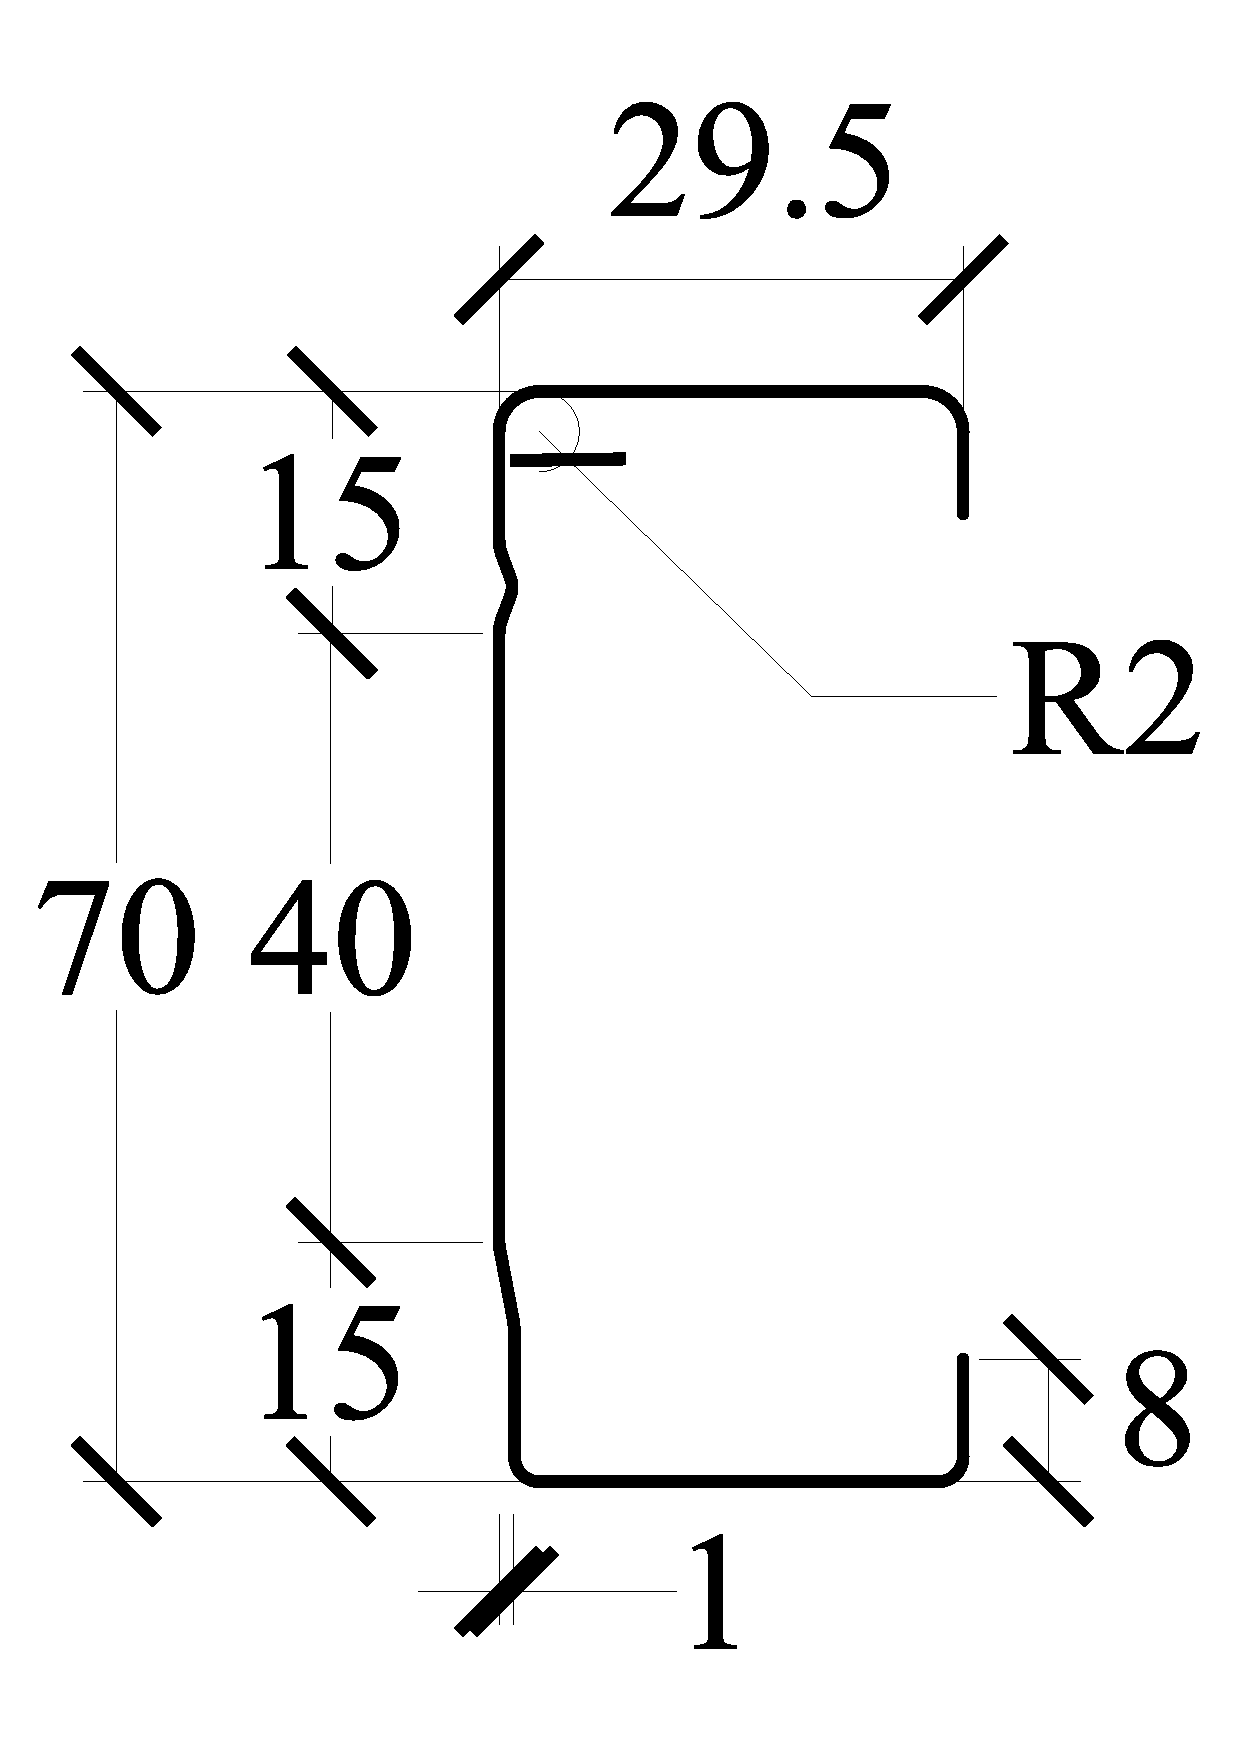
\includegraphics[width=\textwidth]{70mm-stud-section.pdf}
		\caption{}
		\label{subfig:70mm-section}
	\end{subfigure}
	\begin{subfigure}[b]{0.3\textwidth}
		\centering
		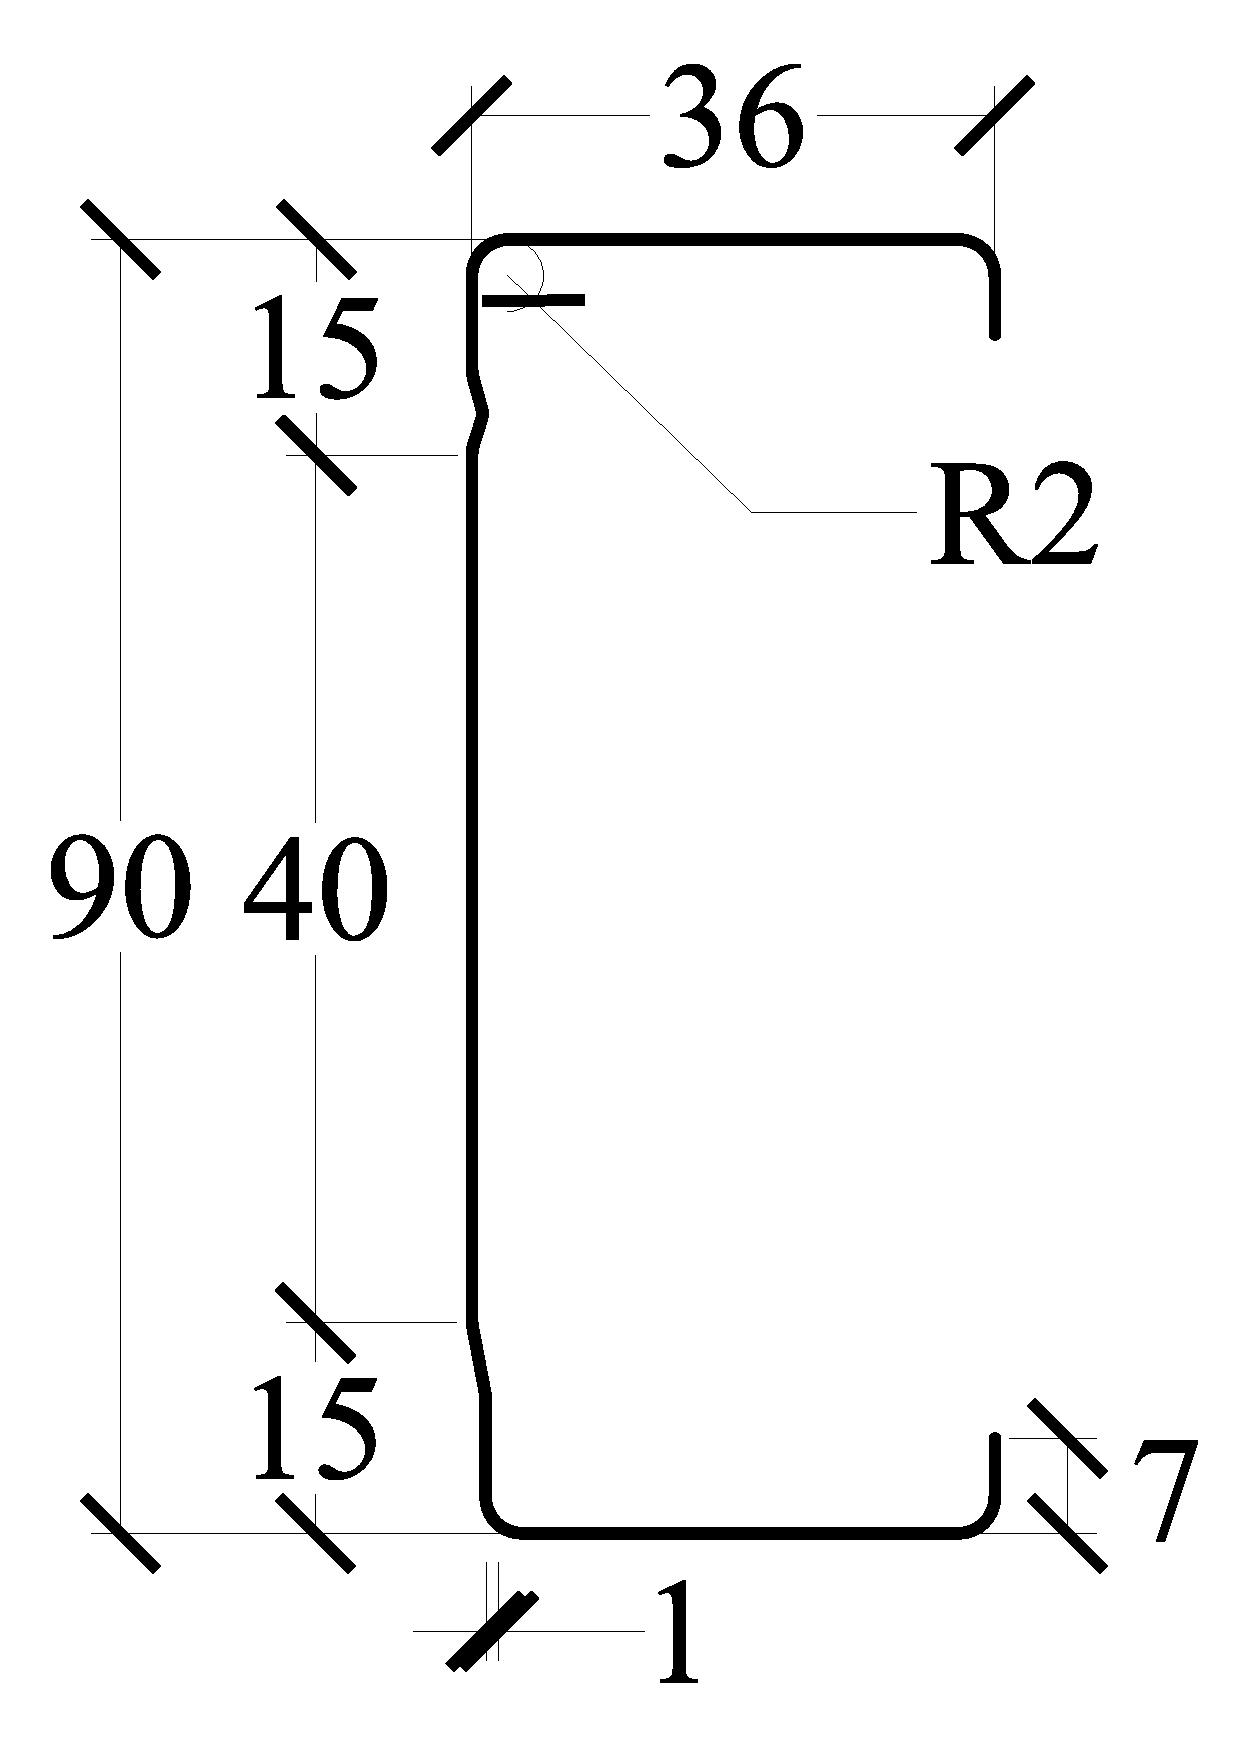
\includegraphics[width=\textwidth]{90mm-stud-section.pdf}
		\caption{}
		\label{subfig:90mm-section}
	\end{subfigure}
	   \caption{Cross-section of (a) 70mm stud (b) 90 mm stud}
	   \label{fig:stud-cross-section}
\end{figure}
\begin{figure}
	\centering
	\begin{subfigure}[b]{0.75\textwidth}
		\centering
		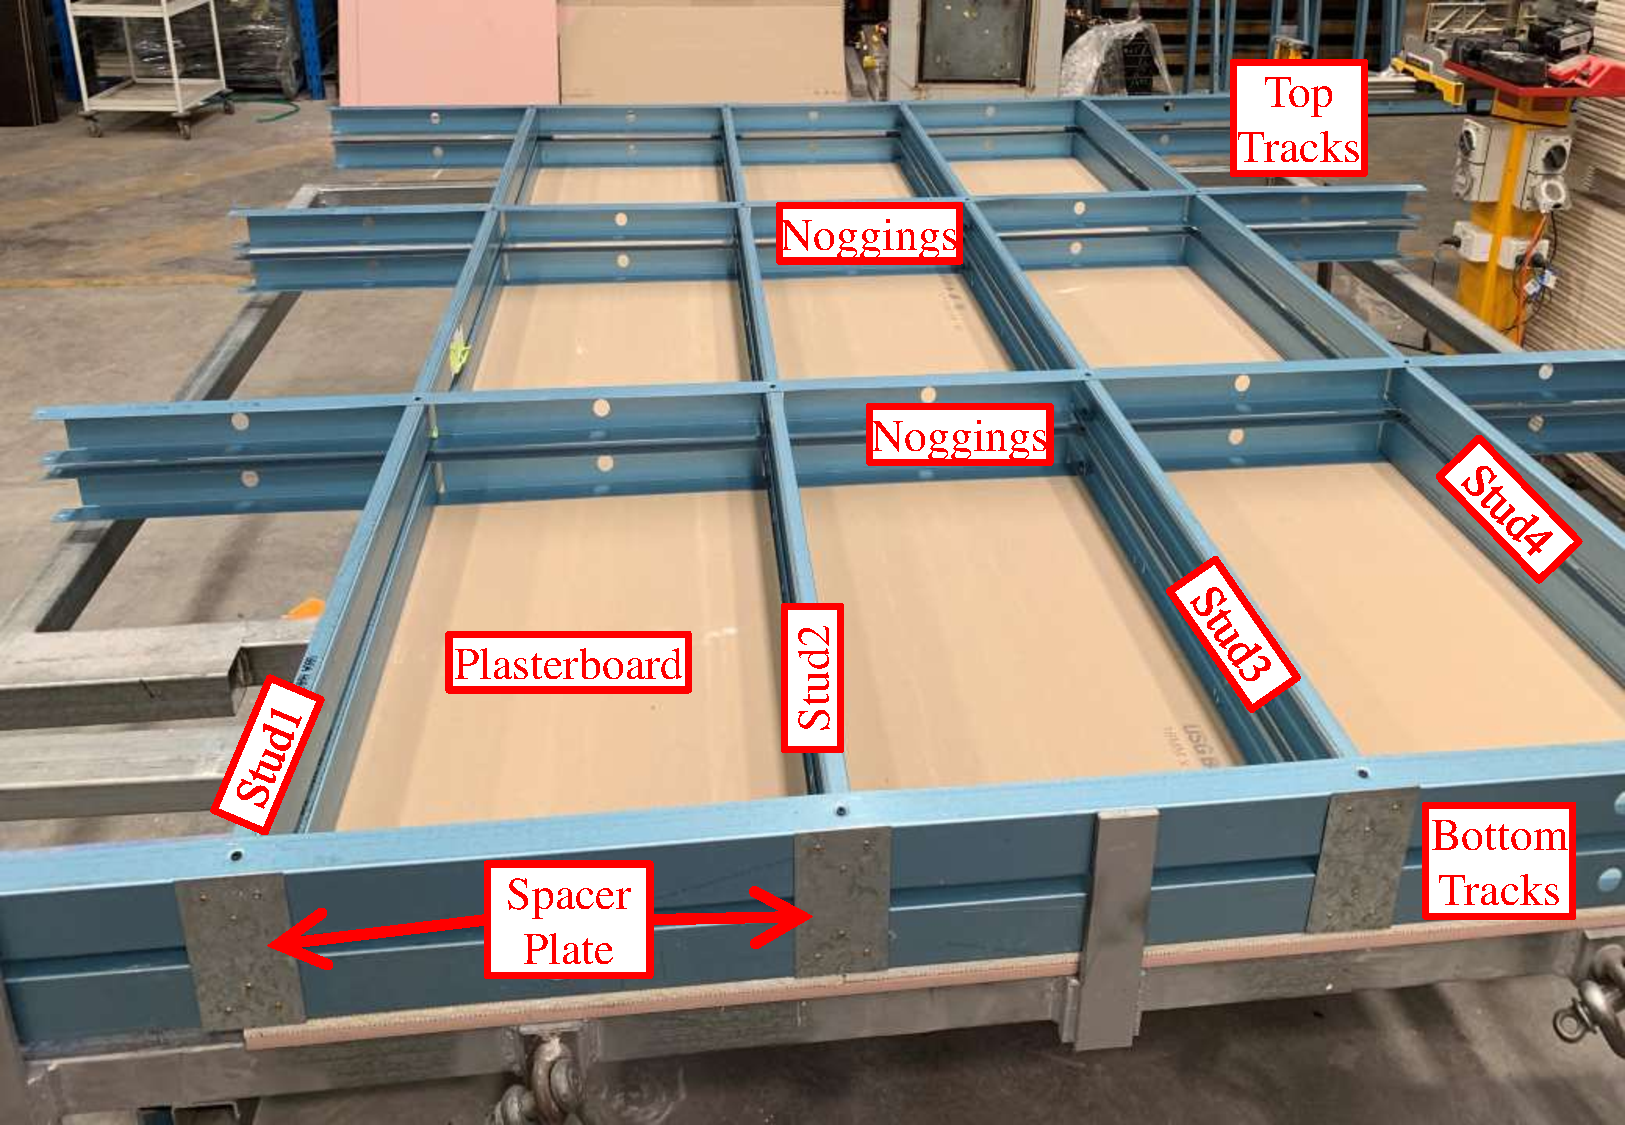
\includegraphics[width=\textwidth]{ambient_construction.pdf}
		\caption{}
		\label{subfig:ambient_construction}
	\end{subfigure}
	\begin{subfigure}[b]{0.75\textwidth}
		\centering
		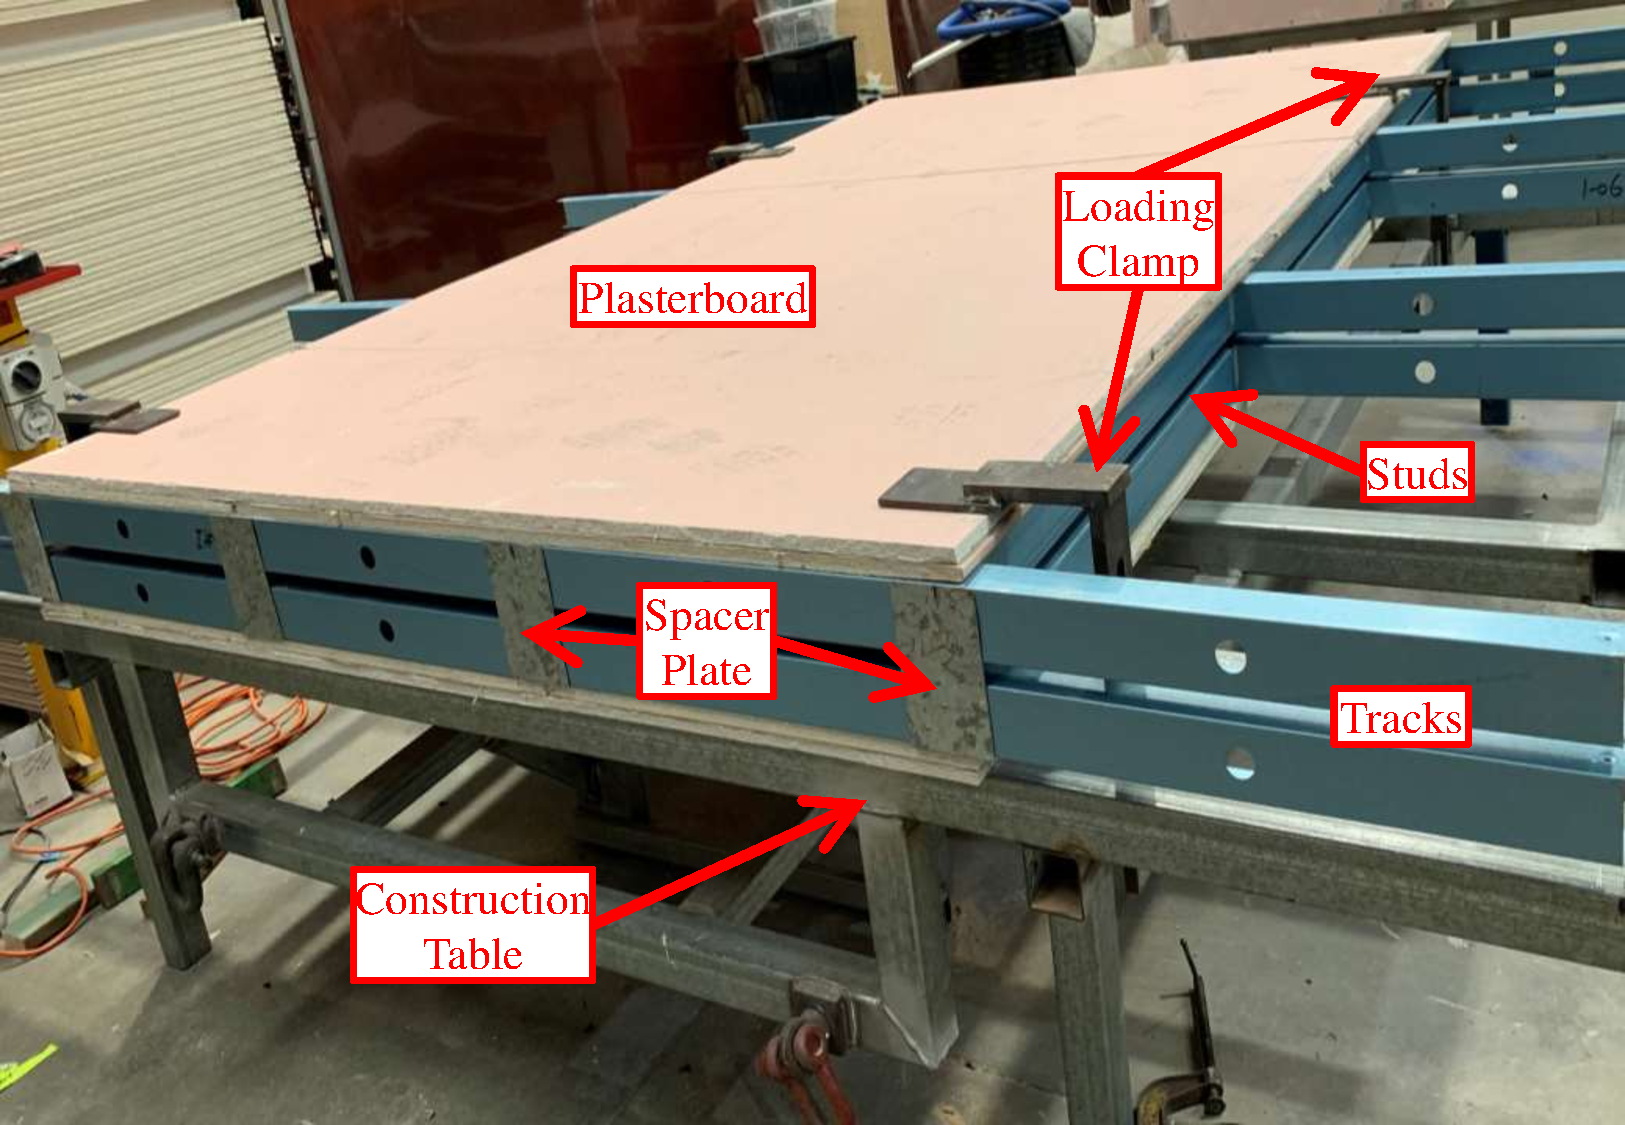
\includegraphics[width=\textwidth]{ambient_finished.pdf}
		\caption{}
		\label{subfig:ambient_finished}
	\end{subfigure}
	   \caption{Construction and testing of LSF wall panels (a) Construction (b) Finished test wall}
	   \label{fig:typical-ambient}
\end{figure}
\begin{figure}[htbp]
	\centering
			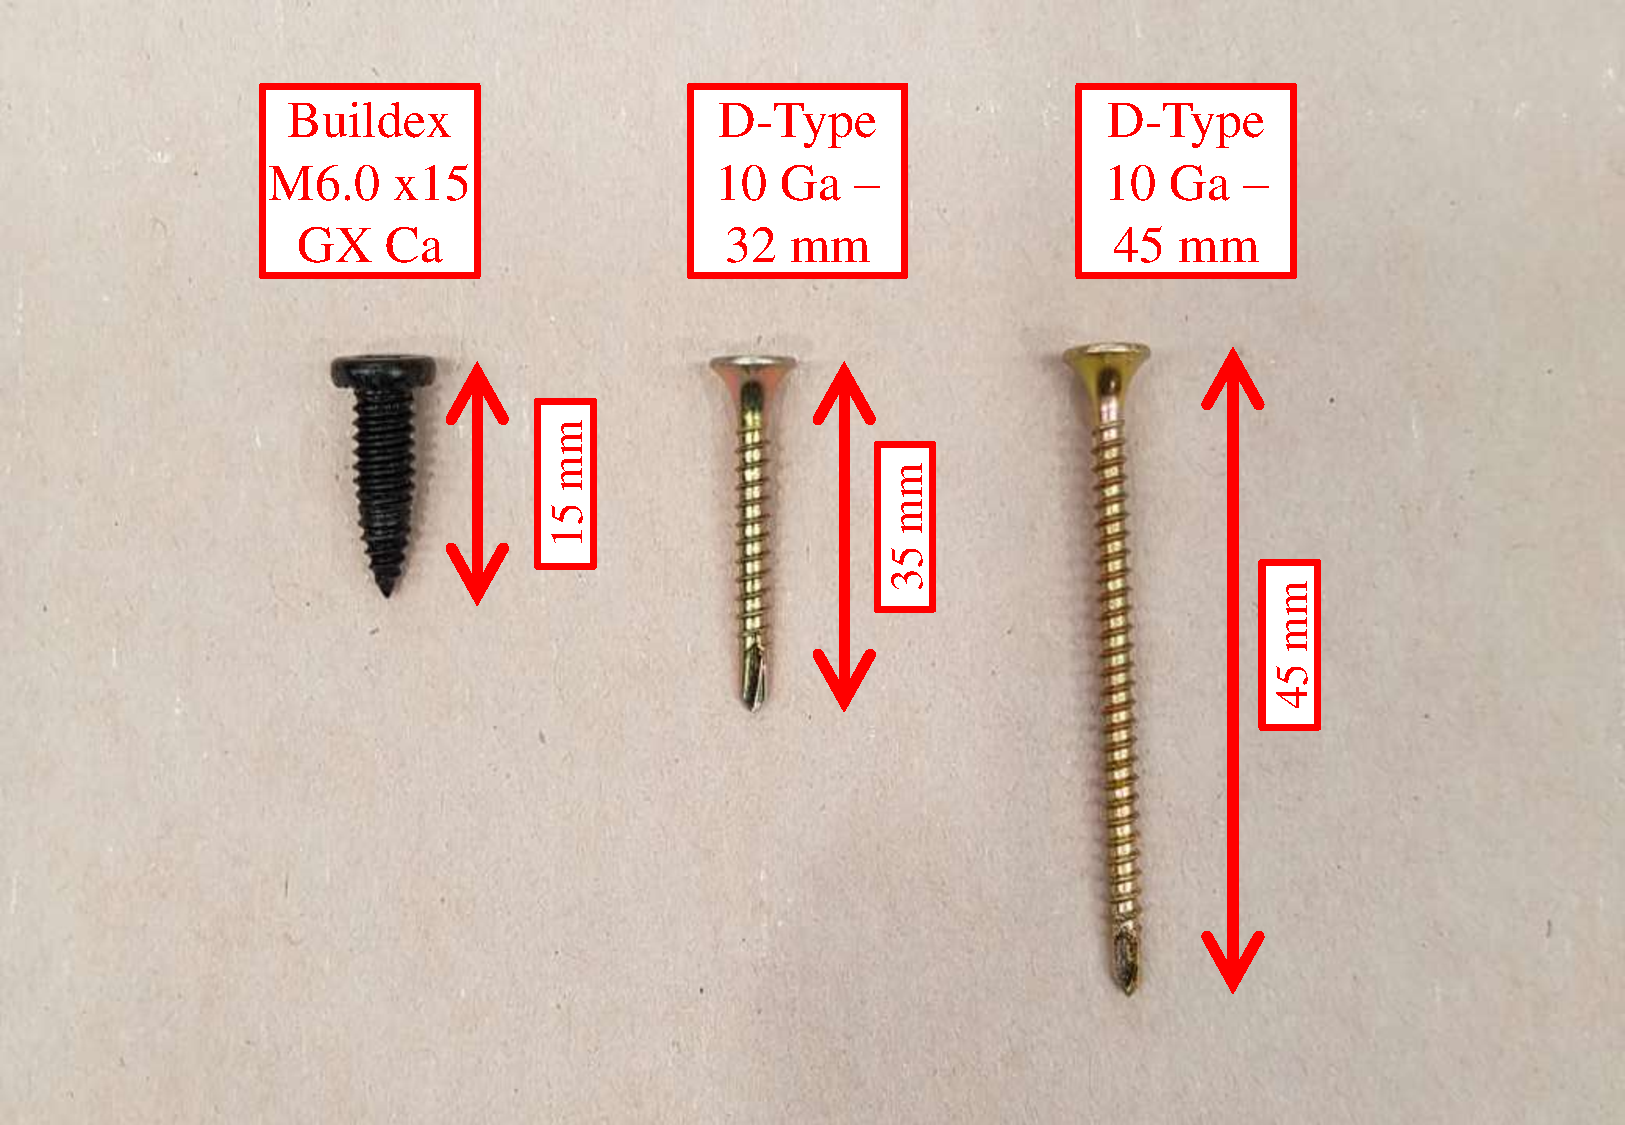
\includegraphics[width=7cm,height=4.5cm]{screws.pdf}
		\caption{Screw details}
		\label{fig:screw-details}
\end{figure}
\begin{figure}
	\centering
	\begin{subfigure}[b]{0.75\textwidth}
		\centering
		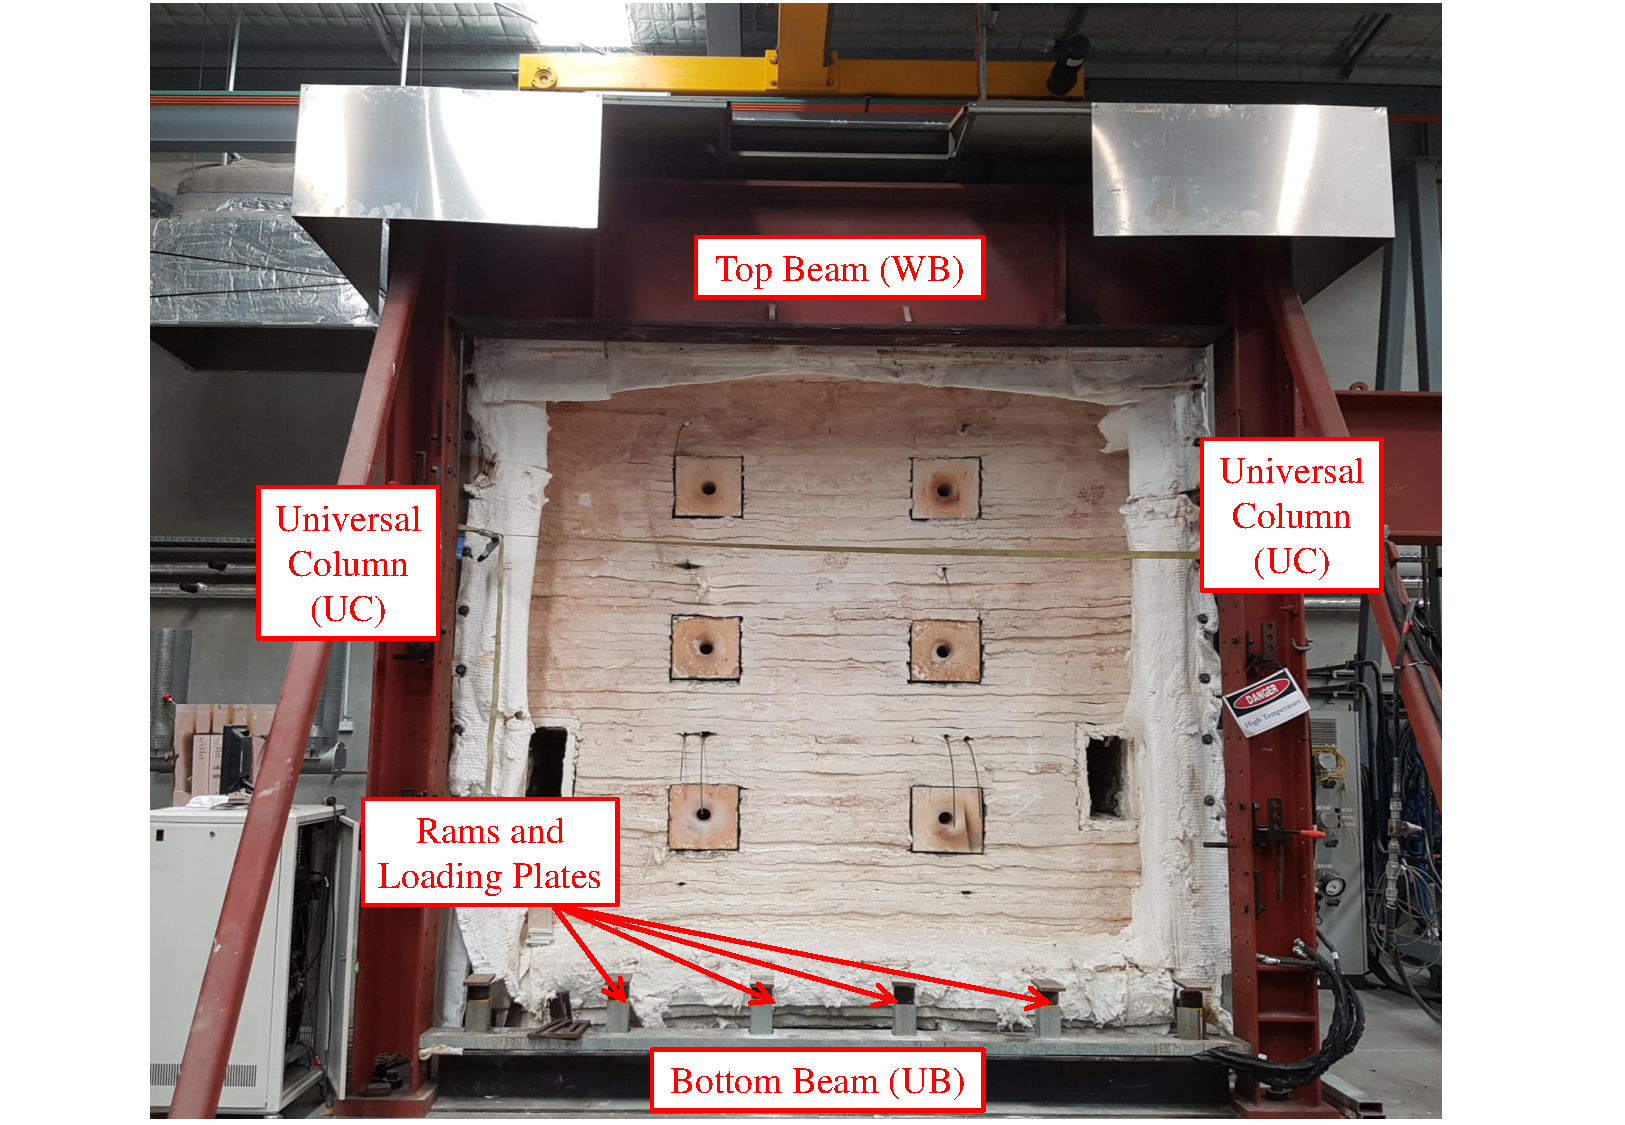
\includegraphics[width=\textwidth]{ambient-loading-frame.pdf}
		\caption{}
		\label{subfig:ambient-loading-frame}
	\end{subfigure}
	\begin{subfigure}[b]{0.5\textwidth}
		\centering
		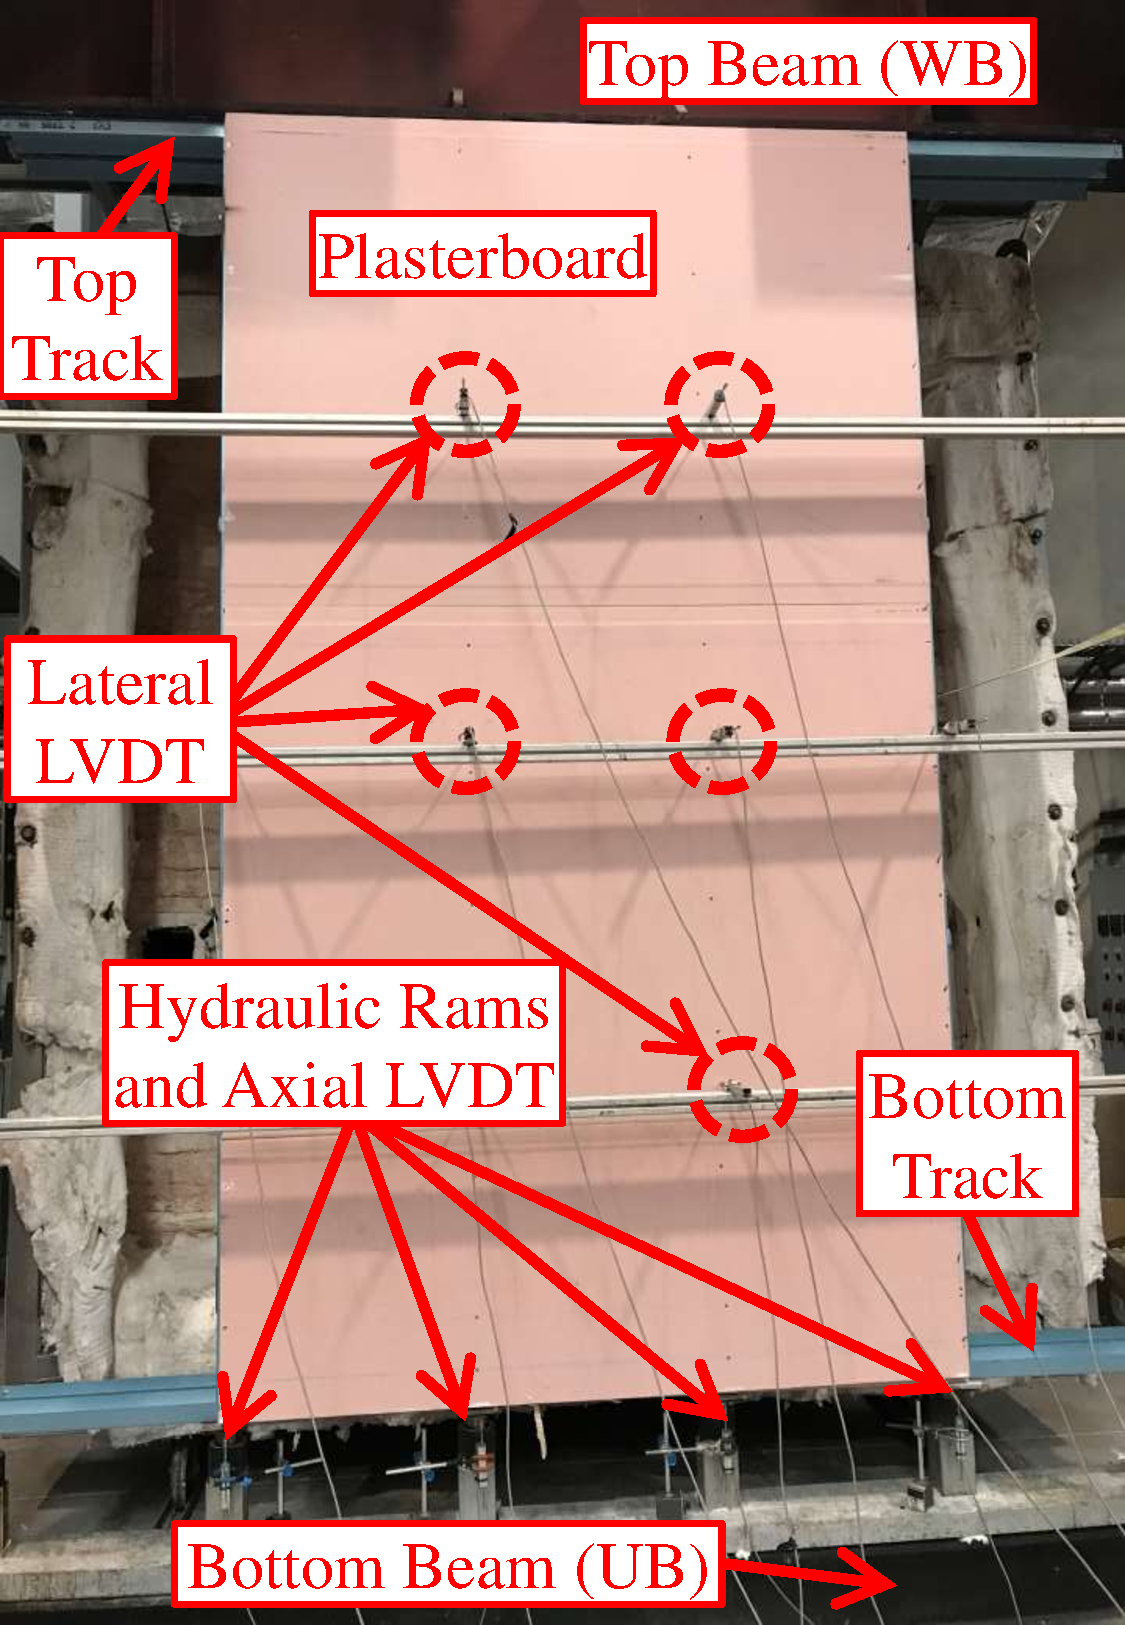
\includegraphics[width=\textwidth]{typical_ambient.pdf}
		\caption{}
		\label{subfig:typical_ambient}
	\end{subfigure}
	%    \caption{Typical loading set-up (a) Test rig (b) Test wall set-up}
	   \label{fig:typical-loading-a}
\end{figure}
\begin{figure}
	\ContinuedFloat
	\centering
	\begin{subfigure}[b]{0.5\textwidth}
		\centering
		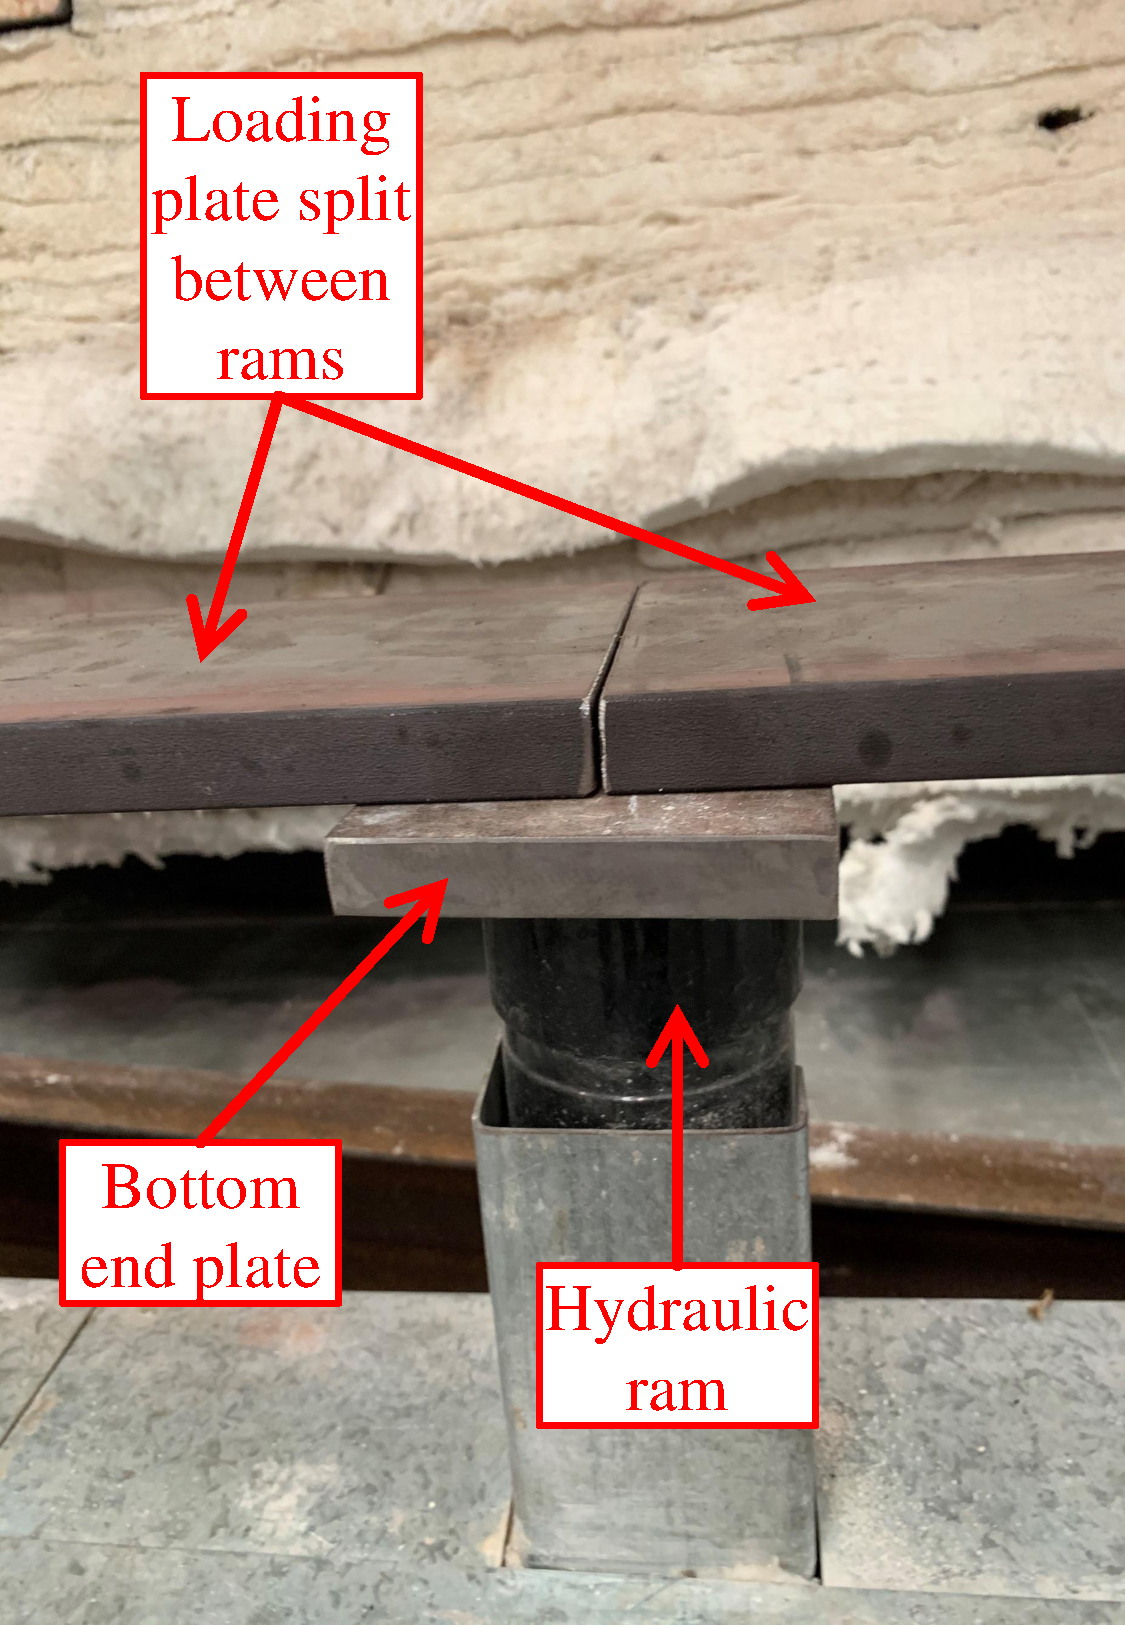
\includegraphics[width=\textwidth]{staggered-loading-detail.pdf}
		\caption{}
		\label{subfig:staggered-loading-detail}
	\end{subfigure}
	\begin{subfigure}[b]{0.75\textwidth}
		\centering
		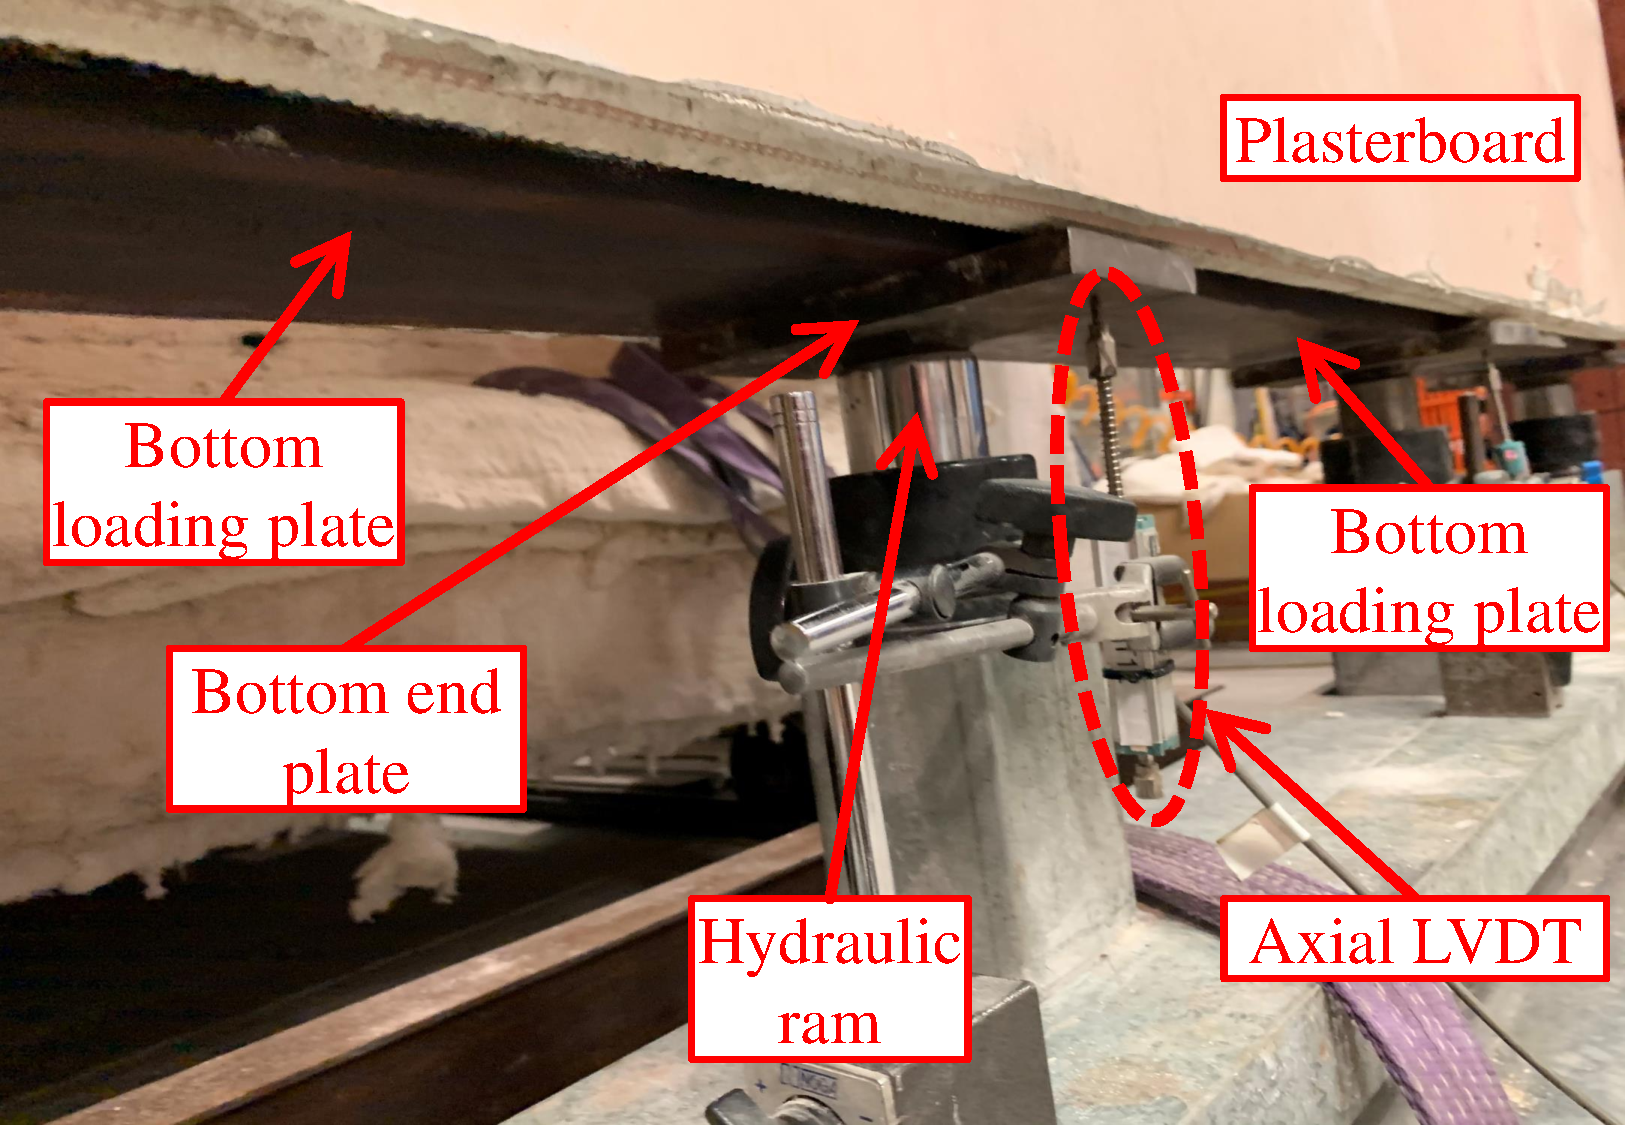
\includegraphics[width=\textwidth]{staggered-loading-arrangement.pdf}
		\caption{}
		\label{subfig:staggered-loading-arrangement}
	\end{subfigure}
	   \caption{Typical loading set-up (a) Test rig (b) Test wall set-up (c) Staggered stud loading ram details (d) Staggered stud wall loading arrangement}
	   \label{fig:typical-loading}
\end{figure}

For staggered stud wall Test-AT5 the test set-up was altered by providing a 20 mm thick loading plate between the rams. Total of 5 loading were arranged on six rams as shown in Figures \ref{fig:typical-loading} (c) and (d). This is to facilitate loading to the staggered stud due to the limitation in test set-up. As the rams in the test set-up was linear the bottom loading plate was used to support and load the floating stud between the rams.  

\section{Test-AT1}\label{sec:Test-AT1}

The first ambient temperature capacity test was conducted on a double stud LSF wall constructed with four G550 90 $\times$ 36 $\times$ 7 $\times$ 0.95 mm studs. 90 $\times$ 40 $\times$ 0.95 mm unlipped channel sections (UCS) were used as noggings at 1 m intervals. The noggings were connected to the studs through slots made on the webs of the UCS. Top and bottom of the test wall panel were connected through 90 mm unlipped channel sections. In this test, the test wall had two rows of studs, separated by a 20 mm gap as shown in \Cref{fig:AT1-plan}. The edge studs were strengthened since the plasterboard provided fully effective in-plane restraints only to the middle studs. The height of the test wall panel was 3 m while its width was 1.8 m.
\begin{figure}[!htbp]
	\centering
			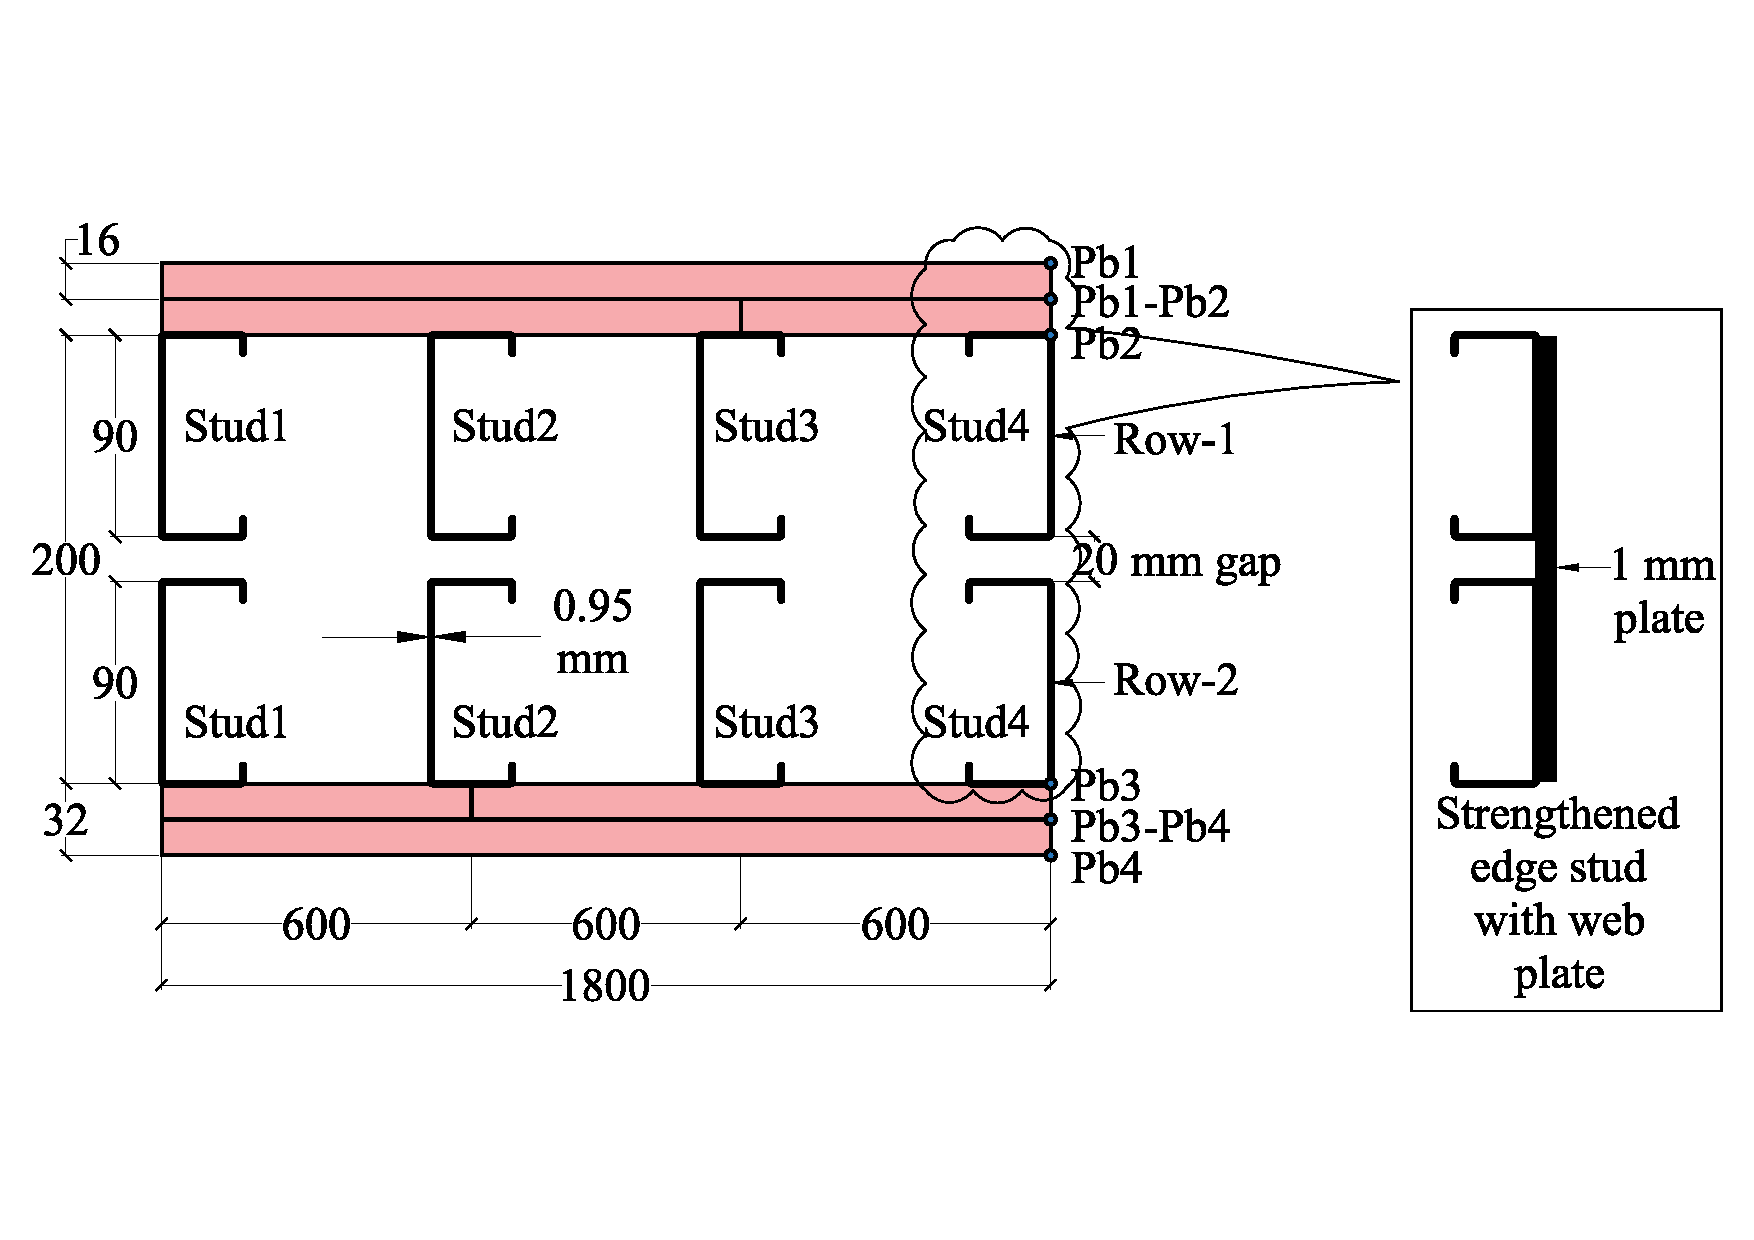
\includegraphics[scale=0.25]{AT1-plan.pdf}\\
		\caption{Test-AT1 wall configuration}
		\label{fig:AT1-plan}
\end{figure} 
\begin{figure}[!htbp]
	\centering
	\begin{subfigure}[b]{0.4\textwidth}
		\centering
		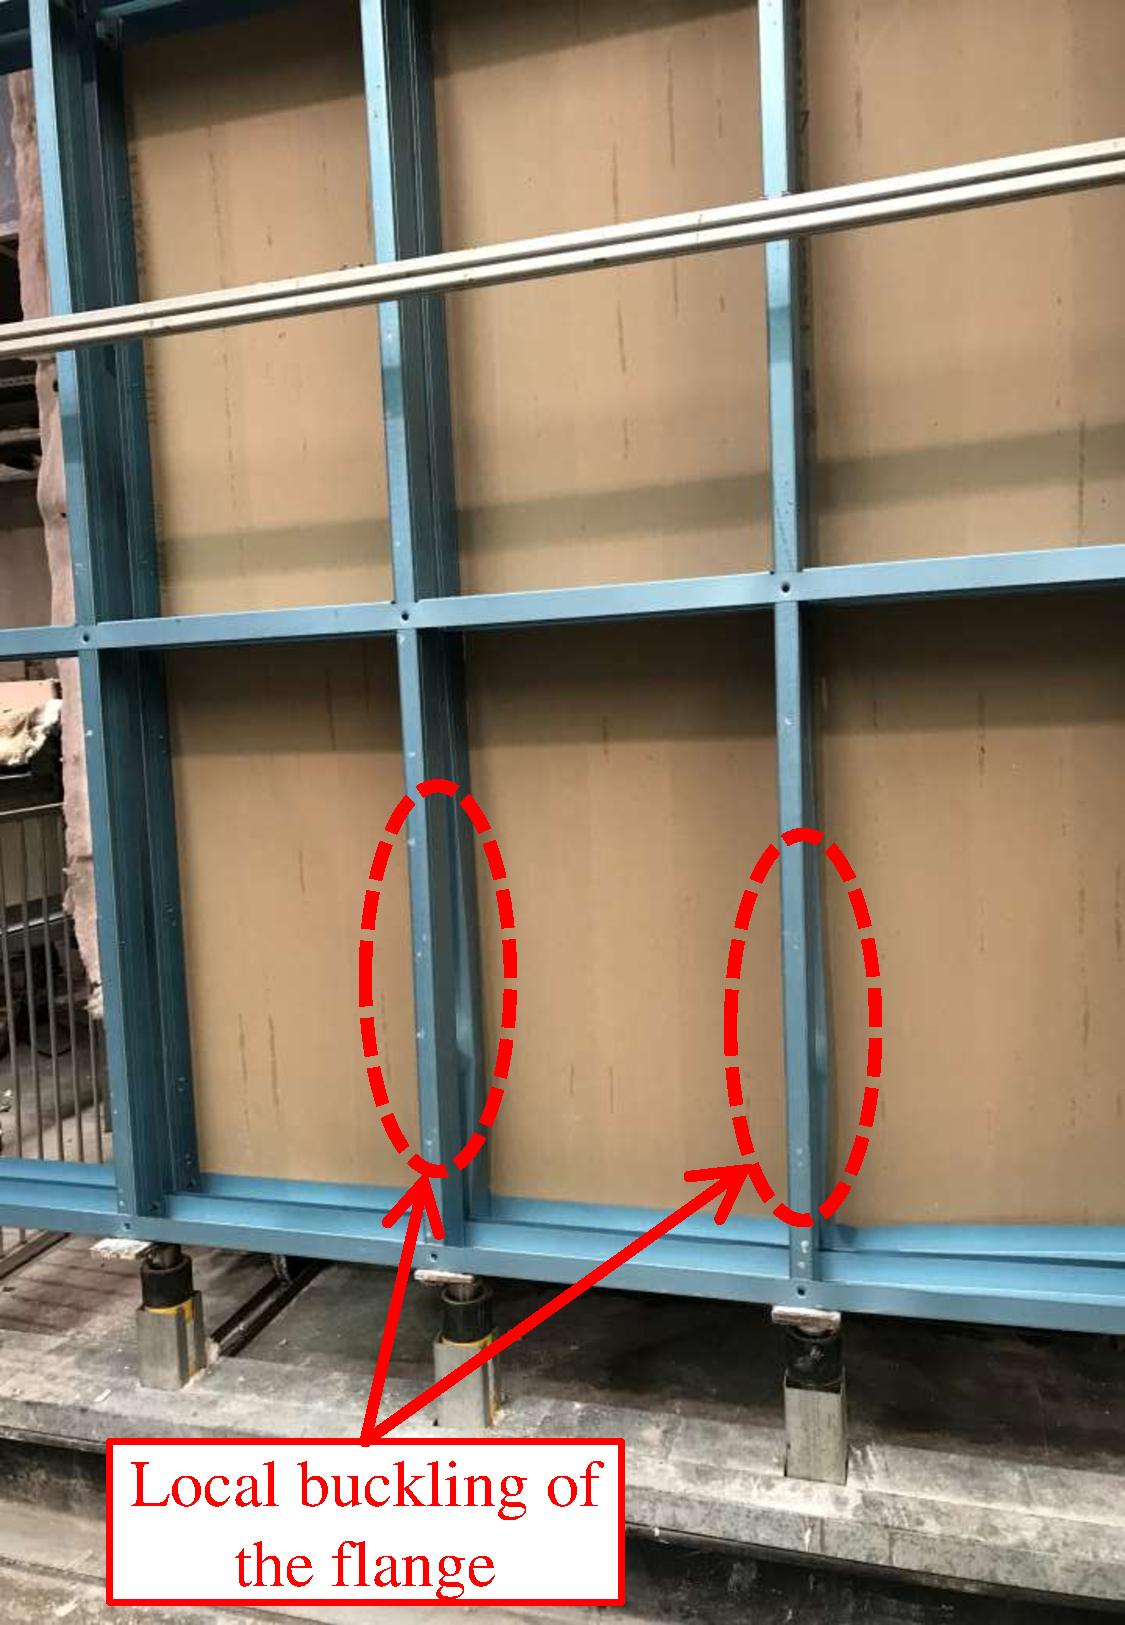
\includegraphics[width=\textwidth]{AT1-full-buckling.pdf}
		\caption{}
		\label{subfig:AT1-full-buckling}
	\end{subfigure}
	\begin{subfigure}[b]{0.4\textwidth}
		\centering
		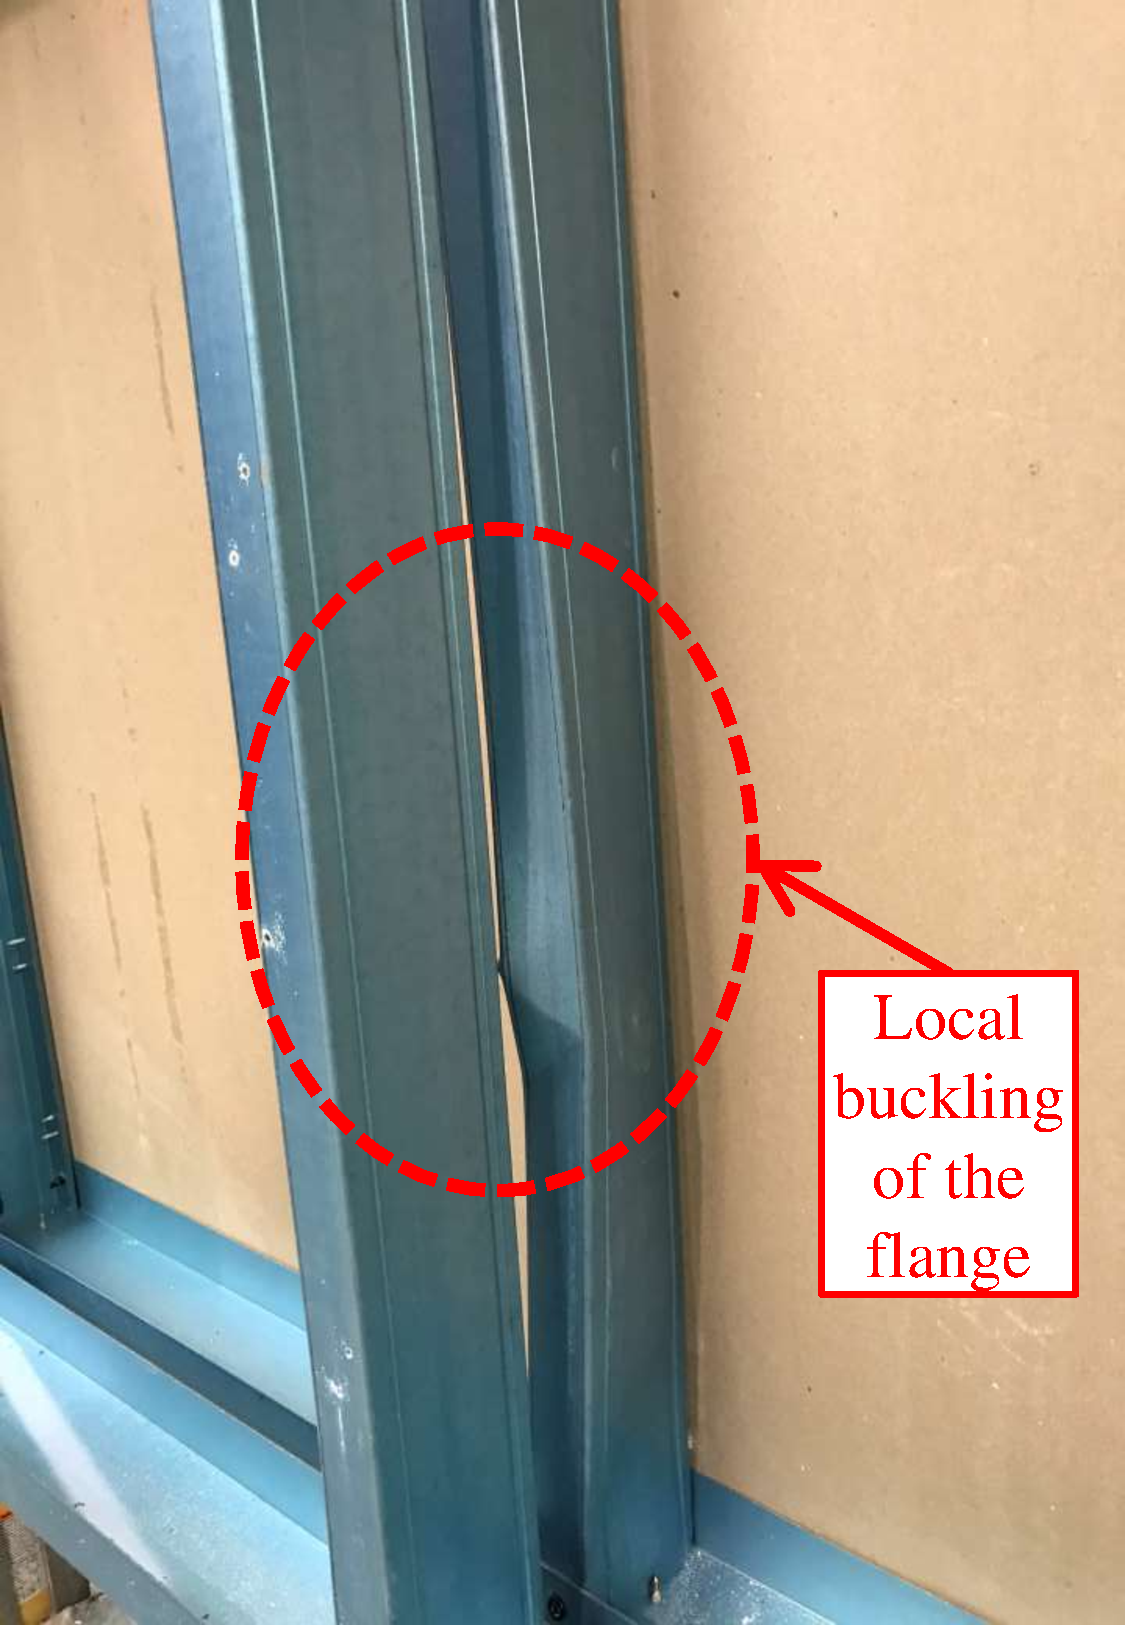
\includegraphics[width=\textwidth]{AT1-buckling.pdf}
		\caption{}
		\label{subfig:AT1-buckling}
	\end{subfigure}
	   \caption{Local compressive failure in Test-AT1 wall (a) Test wall (b) Stud3}
	   \label{fig:AT1-failure}
\end{figure}
\begin{figure}[!htbp]
	\centering
	\begin{subfigure}[b]{0.7\textwidth}
		\centering
		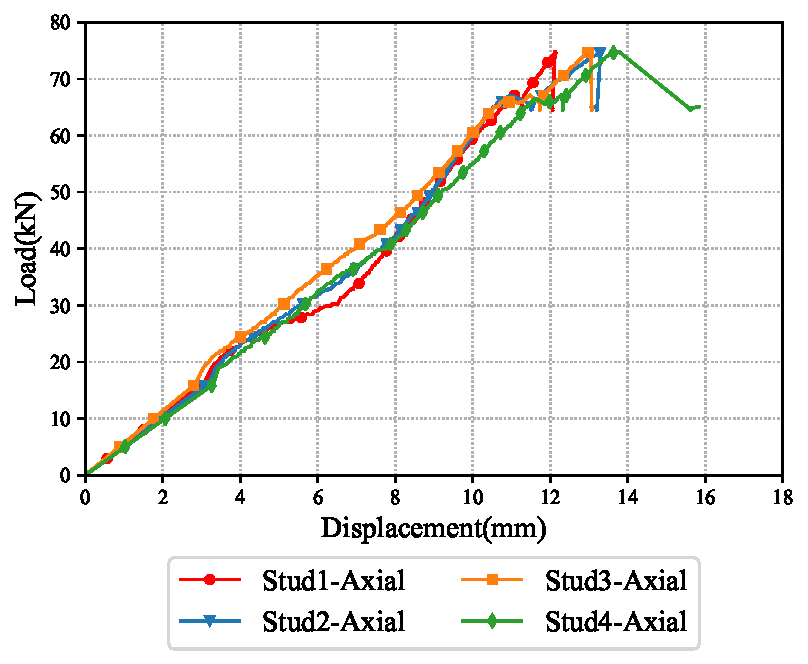
\includegraphics[width=\textwidth]{AT1-Load-Axial-Corrected.pdf}
		\caption{}
		\label{subfig:AT1-Load-Axial-Corrected}
	\end{subfigure}
	\begin{subfigure}[b]{0.7\textwidth}
		\centering
		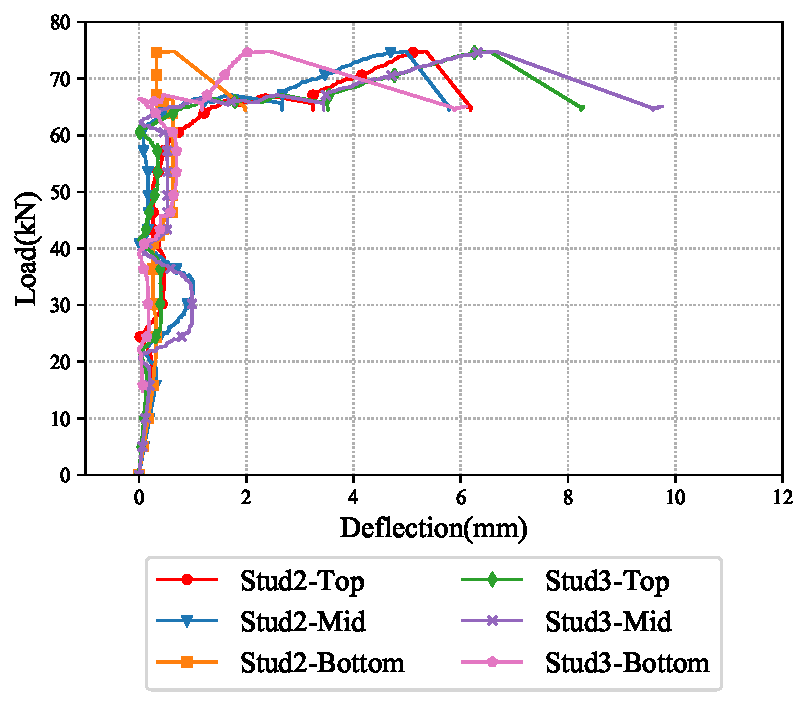
\includegraphics[width=\textwidth]{AT1-Load-Lateral-Corrected.pdf}
		\caption{}
		\label{subfig:AT1-Load-Lateral-Corrected}
	\end{subfigure}
	   \caption{Test-AT1 results - (a) Applied load versus axial displacement and (b) Applied load versus lateral deflection}
	   \label{fig:AT1-results}
\end{figure}

Firstly, the test wall panel was loaded to 10\% of the predicted ambient temperature capacity twice before loading it to failure. The load was applied on the geometric centre of the studs through individual rams as shown in \Cref{subfig:ambient-loading-frame}. Test-AT1 gave an ultimate axial compression capacity of 73 kN when Stud3 of Row-1 failed by local buckling of flanges as shown in Figures \ref{fig:AT1-failure} \subref{subfig:AT1-full-buckling} and (b). No pull-out failures of the plasterboard screws were observed during the test. Generally, in ambient temperature capacity tests the application of load is continued till the ultimate failure load is reached if the monitored load in the data logger displays a sudden drop. The failure was also inferred through visual changes to the test panel which includes cracks on the plasterboard surface due to buckling of studs. The application of load through hydraulic rams is stopped after this stage. Figures \ref{fig:AT1-results} (a) and (b) show the applied axial load versus axial displacement and lateral deflection results from the test wall. A maximum axial displacement of 15.83 mm was observed in Stud4 (\Cref{fig:AT1-results} (a)) while the maximum lateral deflection recorded was 9.75 mm at Stud3-Mid (\Cref{fig:AT1-results} (b)). Buckling of studs was not evident in both rows of stud as the stud flanges have a small difference in their widths. This facilitates the nesting of studs in real world applications, but causes a small eccentricity during axial compression loading resulting in buckling of studs in one row. 

\section{Test-AT2}

The second ambient temperature capacity test was conducted on a four-stud wall constructed of thinner stud sections (0.75 mm G50) with stud dimensions of 90 $\times$ 36 $\times$ 7 $\times$ 0.75 mm. It was conducted to determine the effect of stud thickness on the axial compression capacity of double stud walls. The test specimen was constructed and tested with four studs. The stud dimensions were identical to those of Test-AT1 wall studs except the stud thickness (0.95 mm versus 0.75 mm) as shown in \Cref{fig:AT2-plan}. Testing procedure was similar to that adopted in Test-AT1. Test-AT2 gave an ultimate maximum axial compression capacity of 47.08 kN, when local compressive failure of the flanges in Stud2 of Row-2 occurred as shown in Figures \ref{fig:AT2-failure} (a) and (b). No crack in plasterboards or pull-out failure of screws at the plasterboard connections were observed after the test.  
\begin{figure}[!htbp]
	\centering
			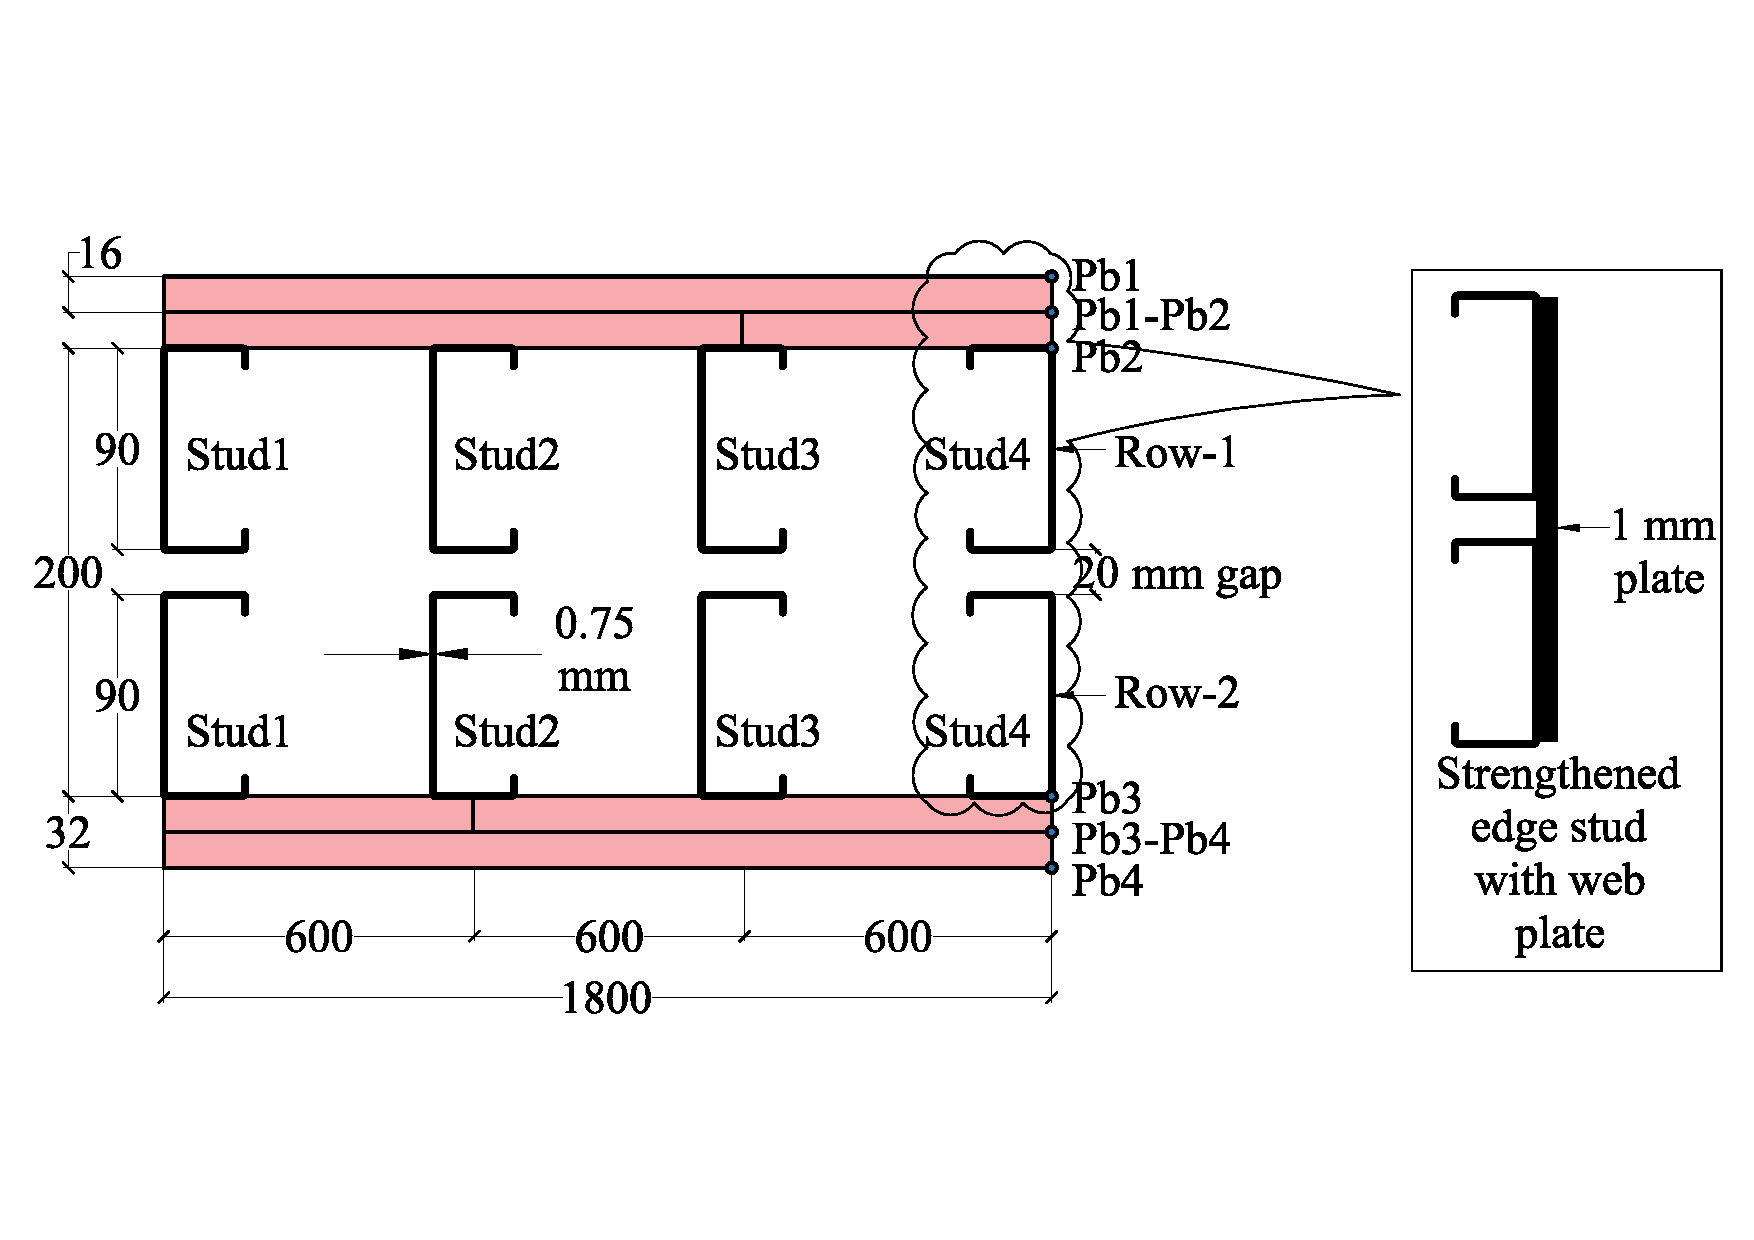
\includegraphics[scale=0.35]{AT2-plan.pdf}\\
		\caption{Test-AT2 configuration}
		\label{fig:AT2-plan}
\end{figure}  
\begin{figure}[!htbp]
	\centering
	\begin{subfigure}[b]{0.4\textwidth}
		\centering
		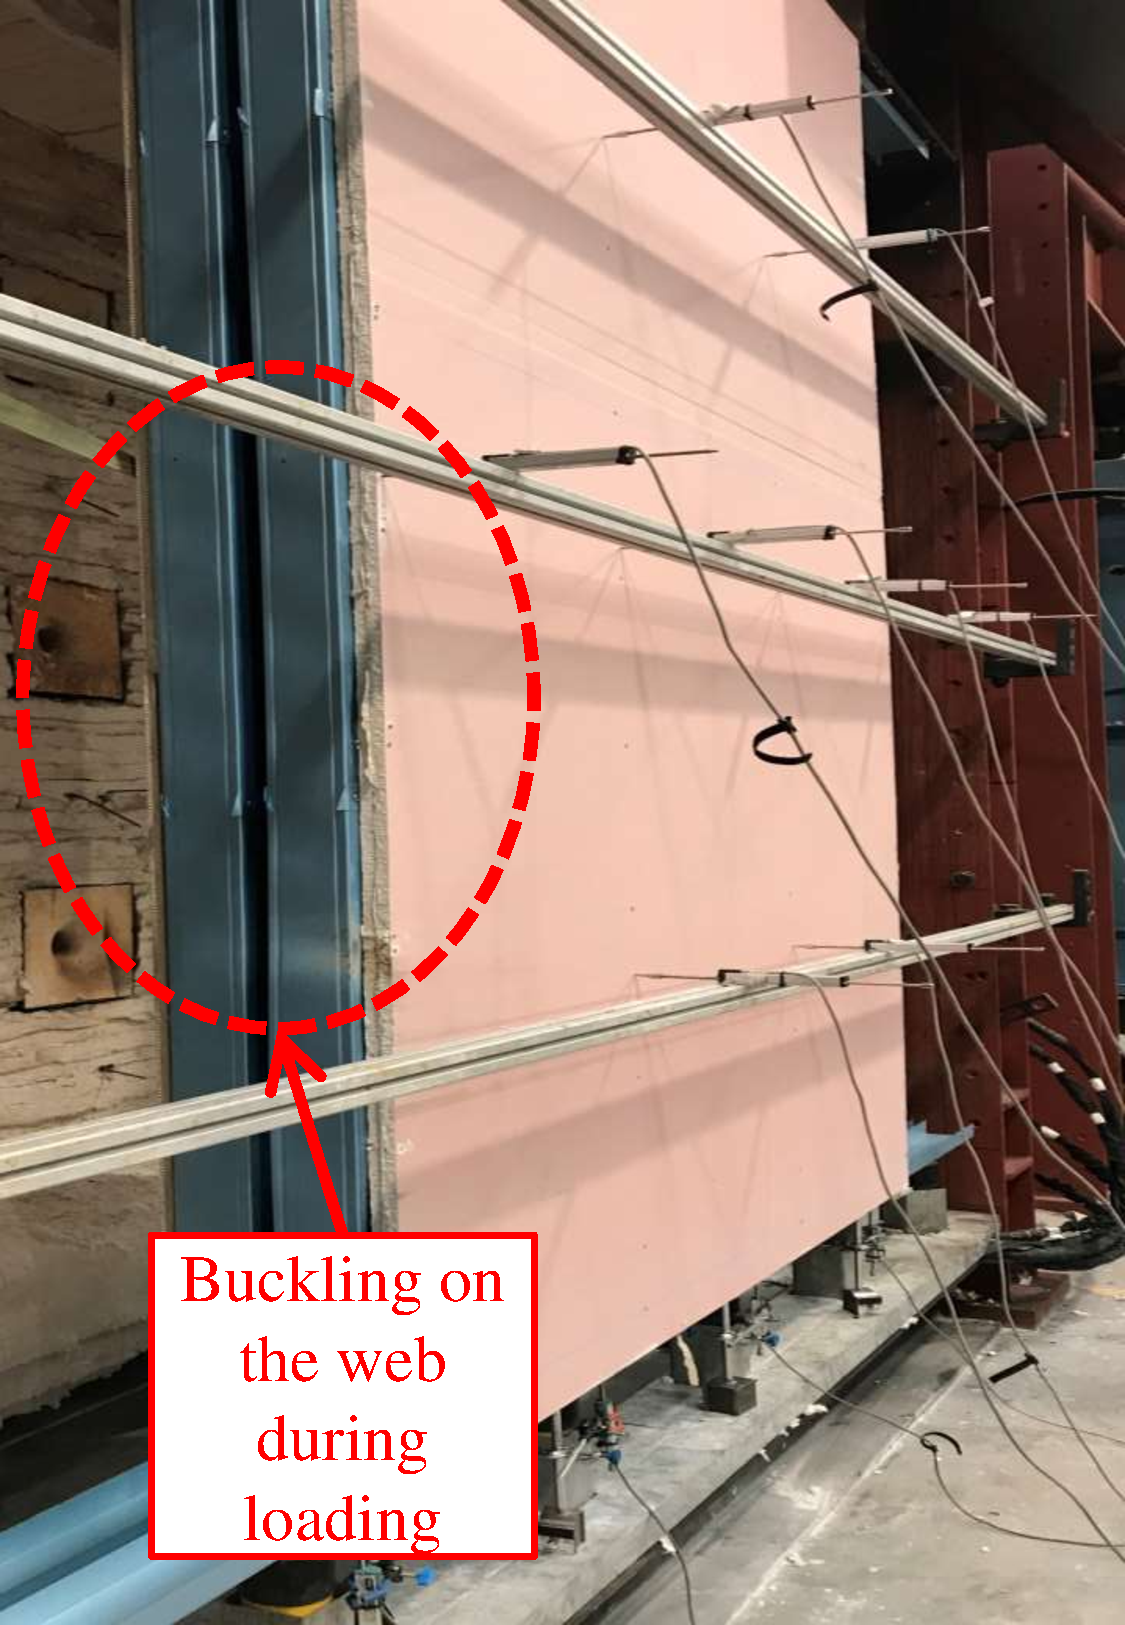
\includegraphics[width=\textwidth]{AT2-full-buckling.pdf}
		\caption{}
		\label{subfig:AT2-full-buckling}
	\end{subfigure}
	\begin{subfigure}[b]{0.4\textwidth}
		\centering
		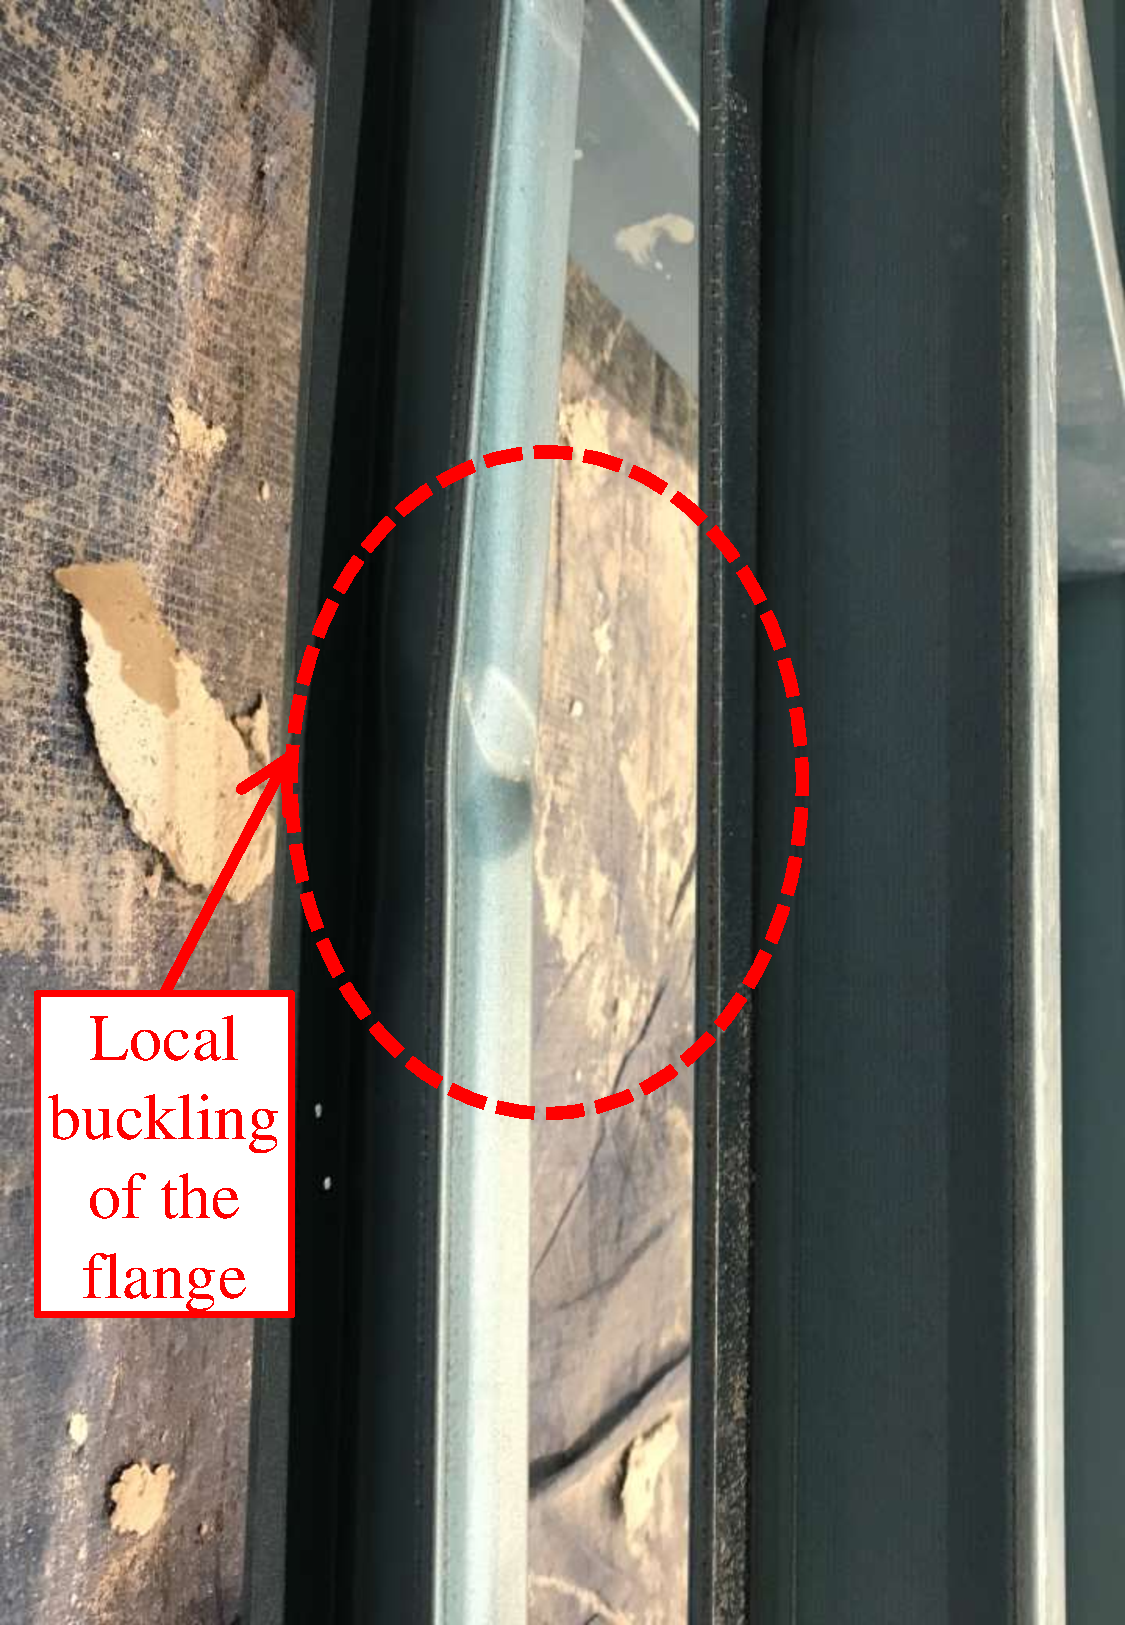
\includegraphics[width=\textwidth]{AT2-buckling.pdf}
		\caption{}
		\label{subfig:AT2-buckling}
	\end{subfigure}
	   \caption{Local compressive failure in Test-AT2 wall (a) Test wall (b) Stud2}
	   \label{fig:AT2-failure}
\end{figure}
\begin{figure}[!htbp]
	\centering
	\begin{subfigure}[b]{0.7\textwidth}
		\centering
		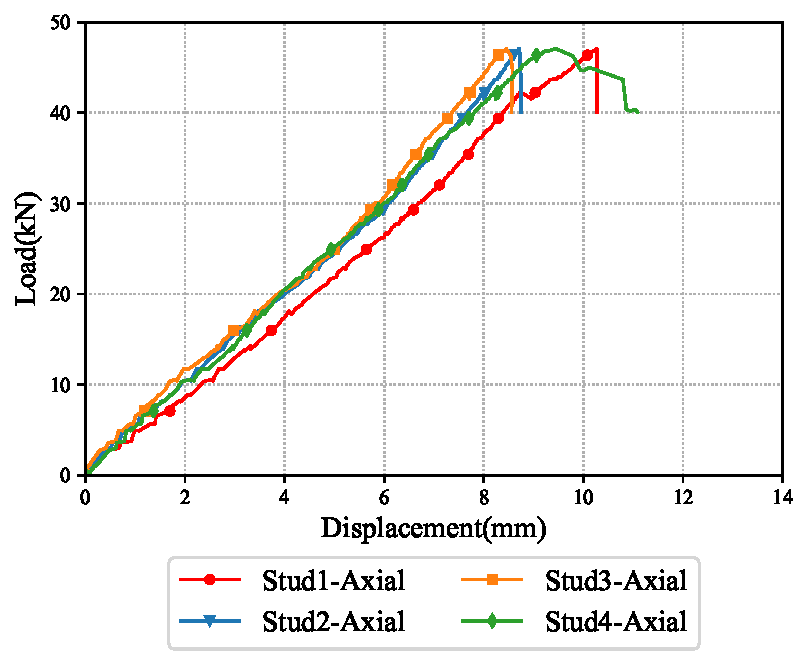
\includegraphics[width=\textwidth]{AT2-Load-Axial-Corrected.pdf}
		\caption{}
		\label{subfig:AT2-Load-Axial-Corrected}
	\end{subfigure}
	\begin{subfigure}[b]{0.7\textwidth}
		\centering
		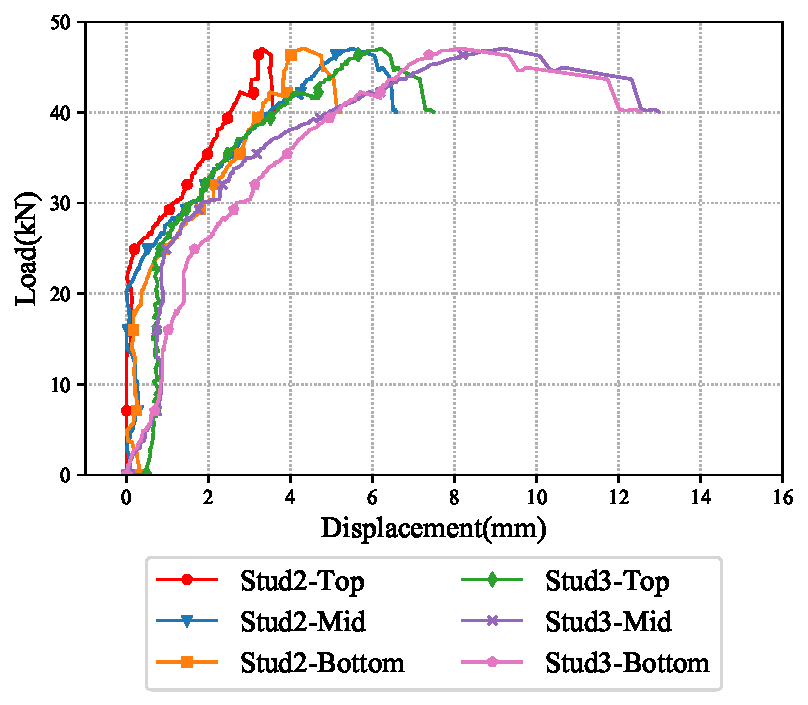
\includegraphics[width=\textwidth]{AT2-Load-Lateral-Corrected.pdf}
		\caption{}
		\label{subfig:AT2-Load-Lateral-Corrected}
	\end{subfigure}
	   \caption{Test-AT2 results - (a) Applied load versus axial displacement and (b) Applied load versus lateral deflection}
	   \label{fig:AT2-results}
\end{figure}

Figures \ref{fig:AT2-results} (a) and (b) show the applied axial load versus the axial displacement and lateral deflection curves from the test. The maximum axial displacement recorded was 11.08 mm as shown in \Cref{fig:AT2-results} (a). A lateral deflection of 12.98 mm at Stud3-Mid was recorded as shown in \Cref{fig:AT2-results} (b). The axial displacement was lesser in comparison to Test-AT1 by 4.75 mm (15.83-11.08 mm). However, the lateral deflections were more by 3.23 mm (12.98-9.75 mm) in comparison with Test-AT1. This is because of the use of thinner stud sections in this test.

\section{Test-AT3}\label{sec:AT3}

The third ambient temperature capacity test was similar to Test-AT2 but had six studs in the test wall. This test was conducted with six studs to verify the axial compression capacity of double stud wall of Test-AT2. \Cref{fig:AT3-plan} shows the test configuration of double stud wall tested with six studs. Despite having six studs in the test wall, fully effective in-plane restraints were available only to the four studs in the middle. Similar to the previous ambient temperature capacity tests, after the initial pre-loading cycle, the ambient temperature capacity of the test wall was determined by applying the axial compressive load to the individual studs until one or more studs failed. The test wall gave an ultimate axial compression capacity of 39.42 kN. No significant buckling was observed in others studs as shown in \Cref{fig:AT3-buckling} (a). However, local bearing failure was observed in the edge stud as shown in \Cref{fig:AT3-buckling} (b). Bearing failure might have occurred in the edge studs due to insufficient plasterboard restraints to the edge studs. The plasterboard restraints provided to the edge studs are not symmetrical in comparison to the middle studs, thereby leaving the edge studs more susceptible to failure. This issue can be addressed by strengthening the edge studs by providing nested or back to back stud sections in ambient temperature capacity tests. 
\begin{figure}[!htbp]
	\centering
			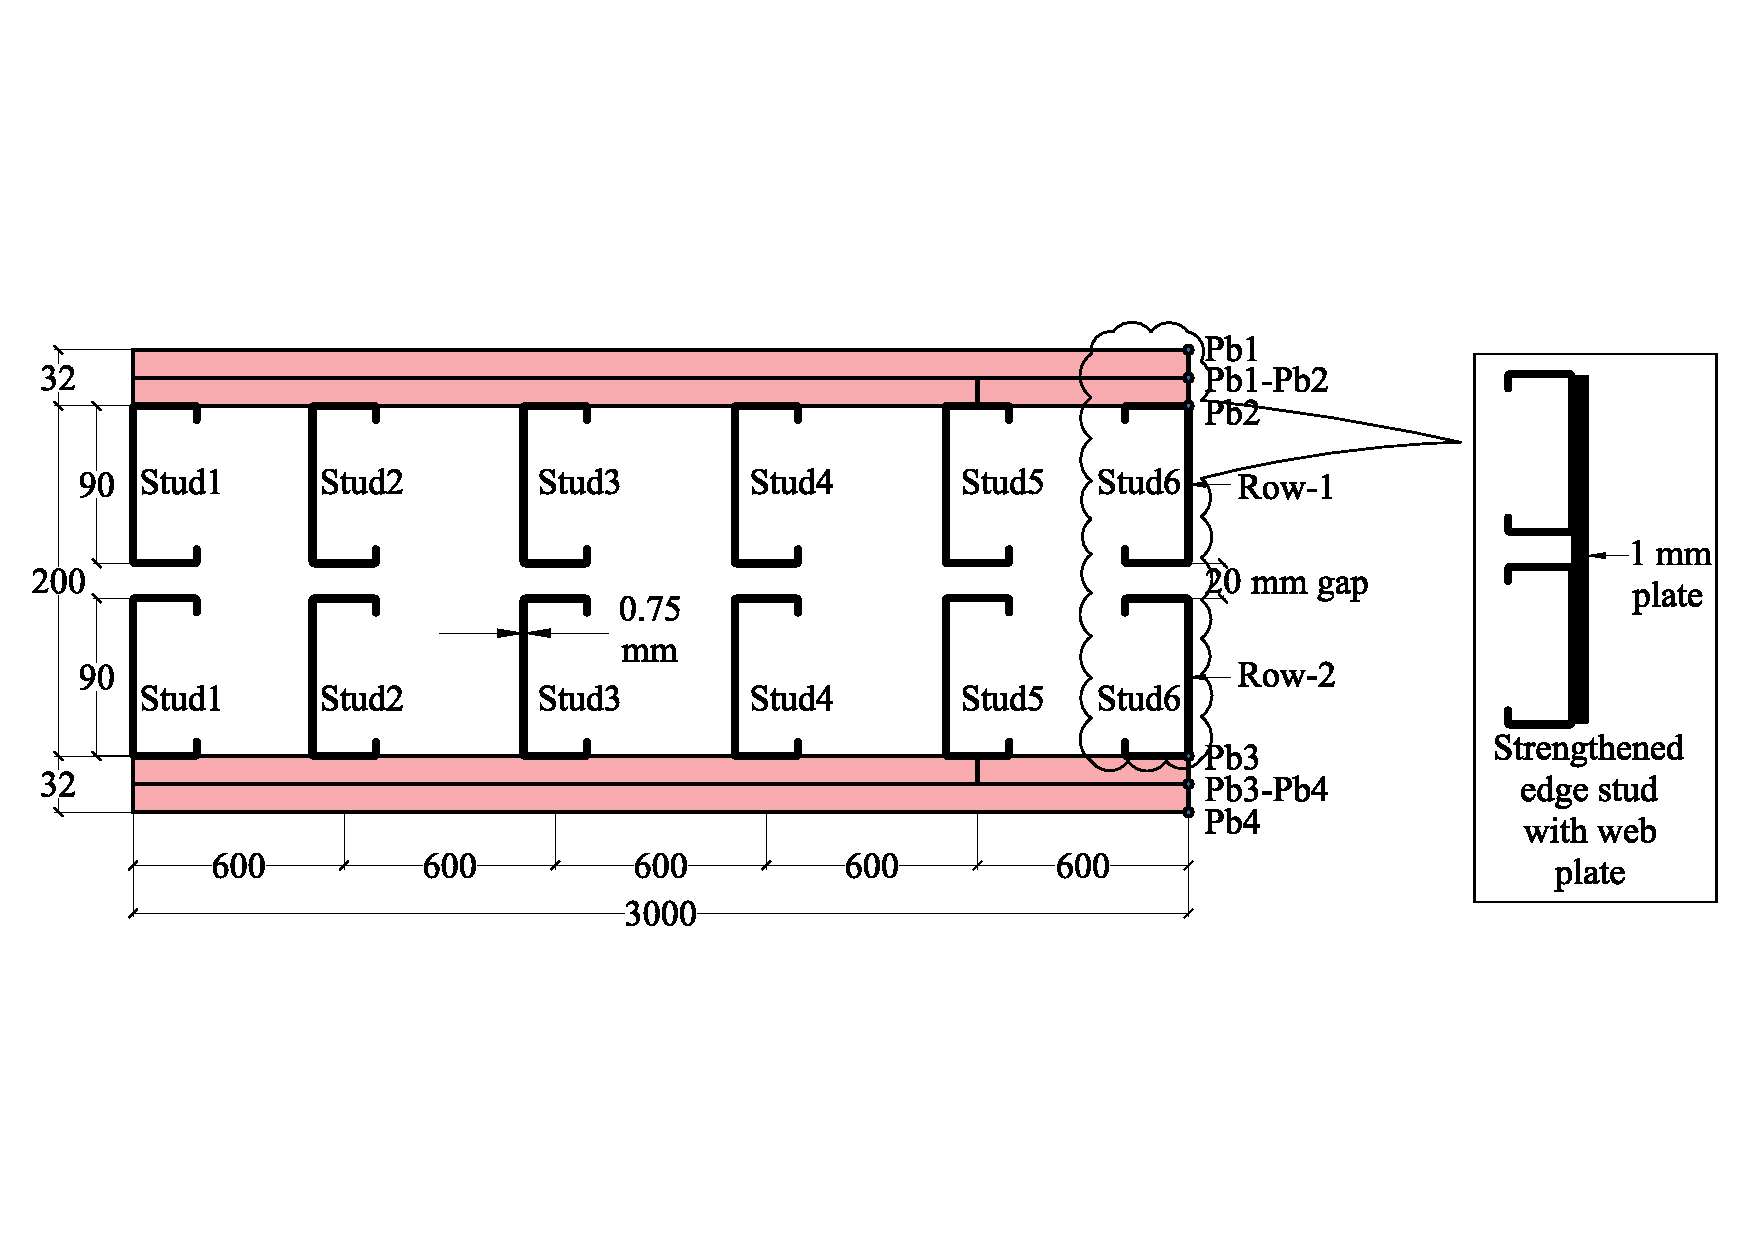
\includegraphics[scale=0.3]{AT3-plan.pdf}\\
		\caption{Test-AT3 configuration}
		\label{fig:AT3-plan}
\end{figure} 
\begin{figure}[!htbp]
	\centering
	\begin{subfigure}[b]{0.6\textwidth}
		\centering
		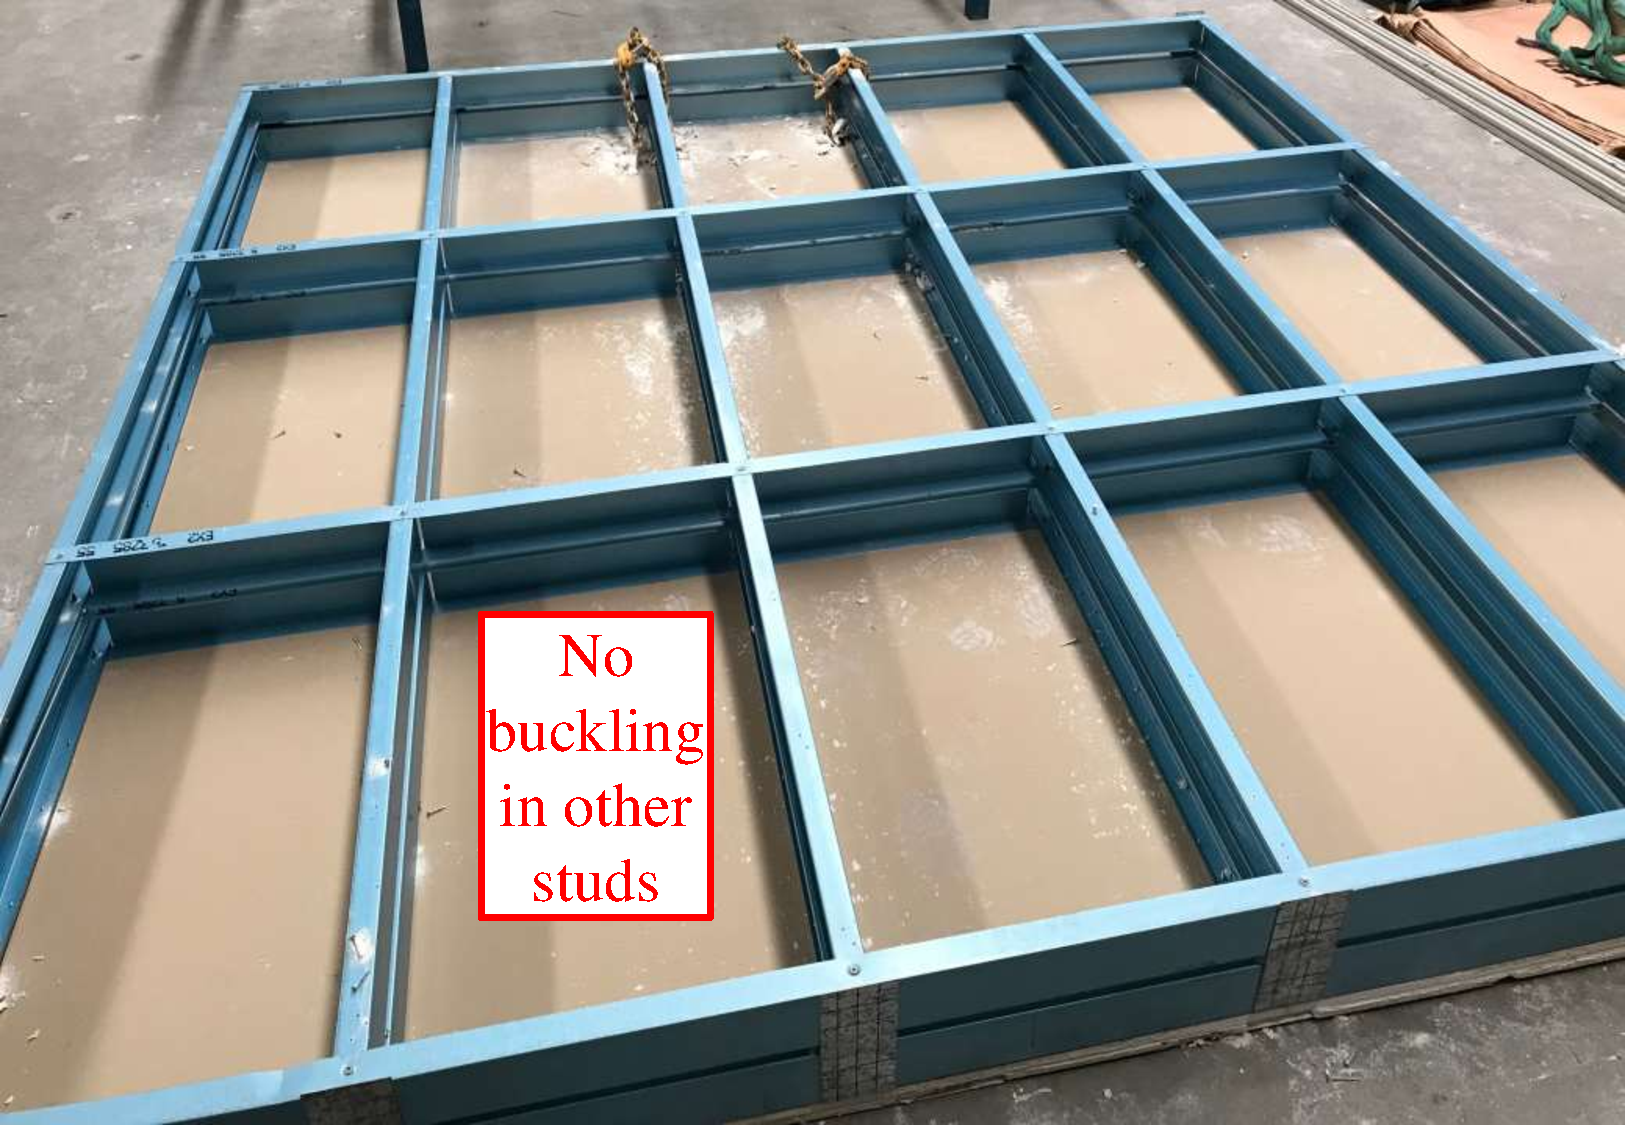
\includegraphics[width=\textwidth]{AT3-buckling.pdf}
		\caption{}
		\label{subfig:AT3-stud-buckling}
	\end{subfigure}
	\begin{subfigure}[b]{0.5\textwidth}
		\centering
		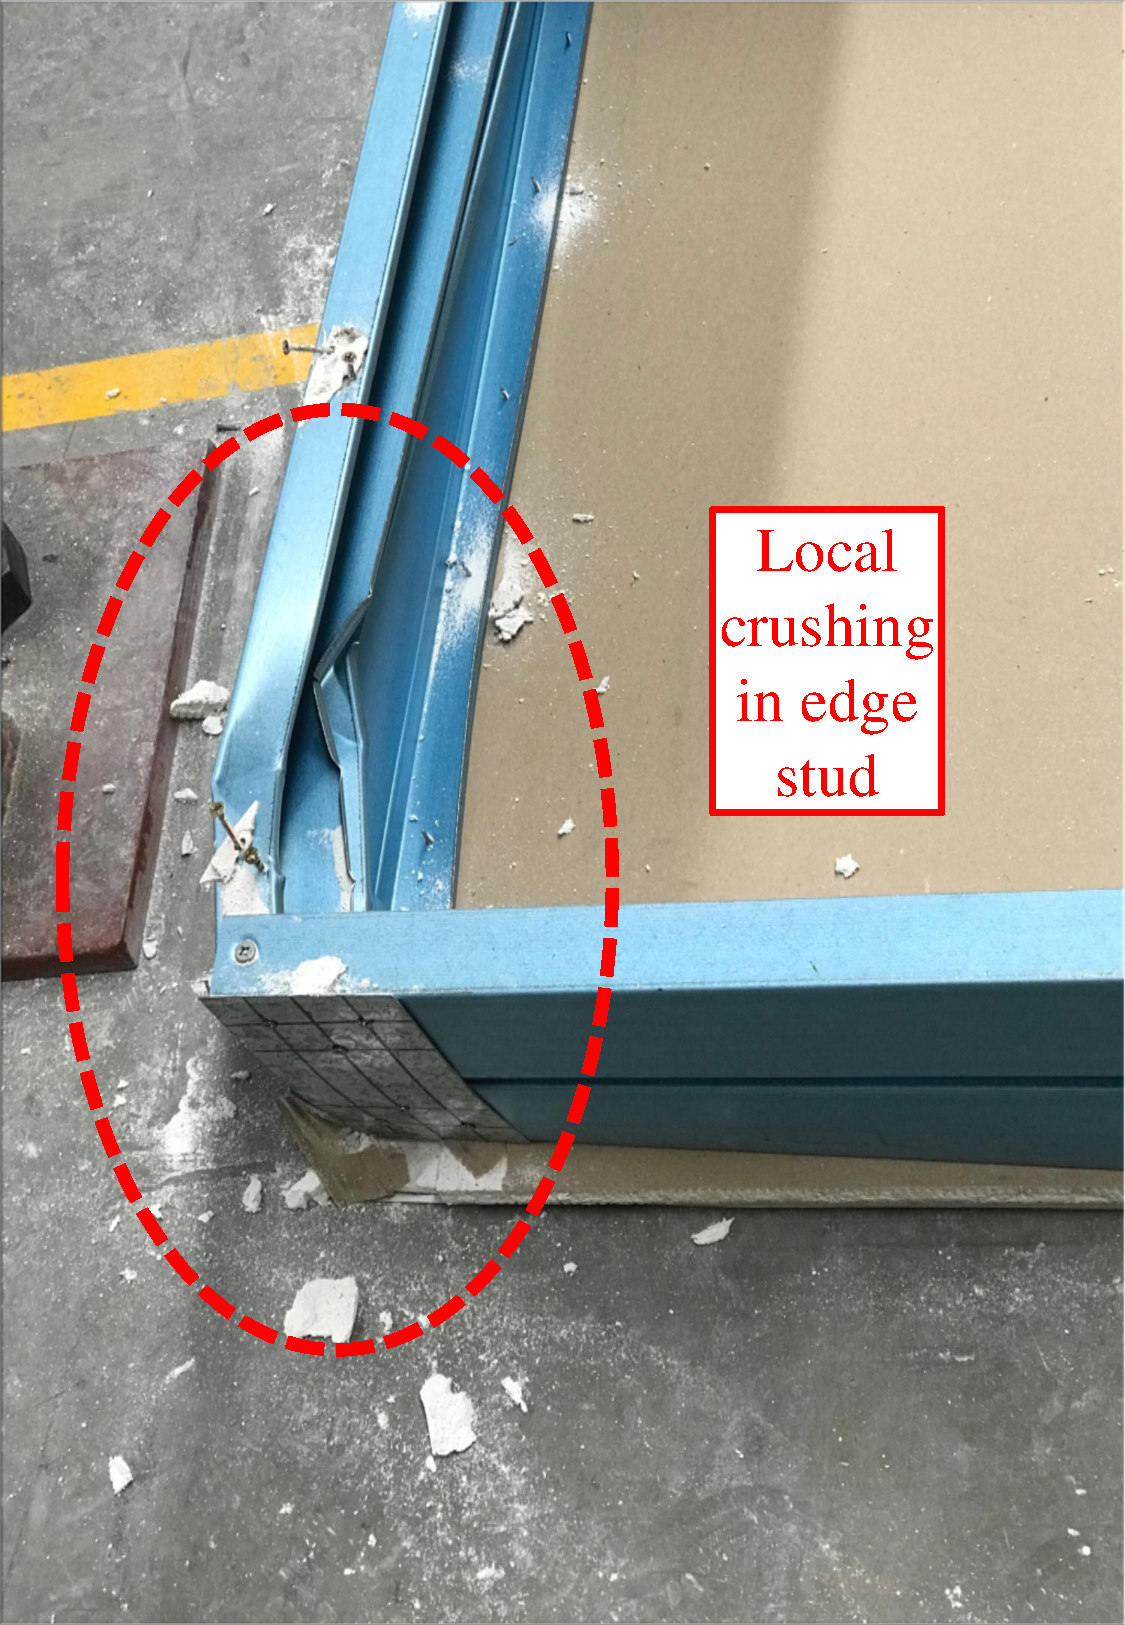
\includegraphics[width=\textwidth]{AT3-stud-crushing.pdf}
		\caption{}
		\label{subfig:AT3-stud-crushing}
	\end{subfigure}
	   \caption{Local bearing failure in Test-AT3}
	   \label{fig:AT3-buckling}
\end{figure} 

Figures \ref{fig:AT3-results} (a) and (b) show the axial displacement and lateral deflection curves. A maximum axial displacement of 9 mm was recorded in Stud2 and a maximum lateral deflection of 6.41 mm was observed at Stud4-Bottom. In comparison with Test-AT2 the axial compression capacity was reduced by 7.66 kN. This was due to the bearing failure of the edge stud in comparison to the local buckling failure of studs in Test-AT2. However, the axial displacement and lateral deflection results were similar in both Tests-AT2 and AT3 (Stud1 and 6) shown in \Cref{fig:AT3-results} (a). This is because, the plasterboards do not provide effective lateral restraints to the edge studs.
\begin{figure}[!htbp]
	\centering
	\begin{subfigure}[b]{0.6\textwidth}
		\centering
		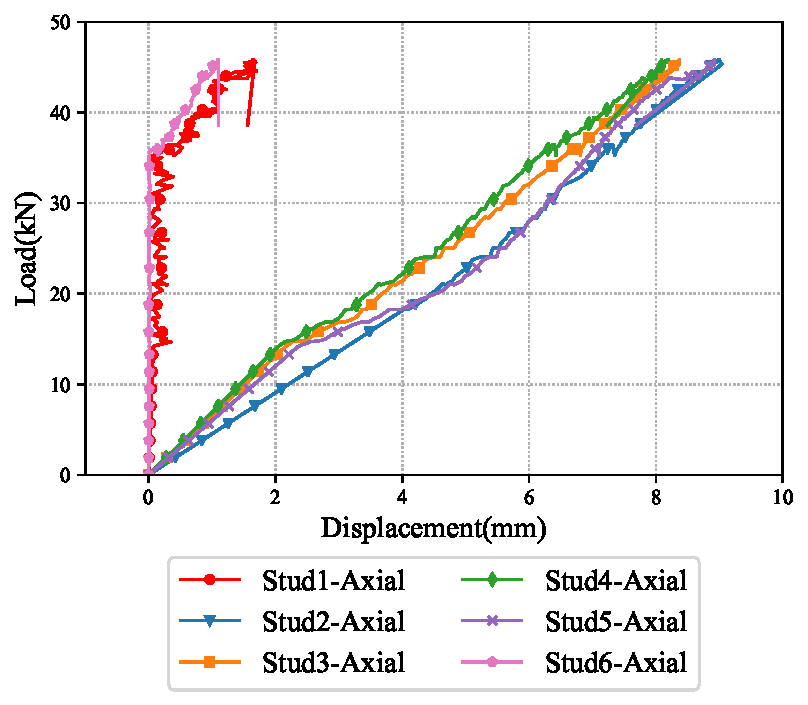
\includegraphics[width=\textwidth]{AT3-Load-Axial-Corrected.pdf}
		\caption{}
		\label{subfig:AT3-Load-Axial-Corrected}
	\end{subfigure}
	\begin{subfigure}[b]{0.6\textwidth}
		\centering
		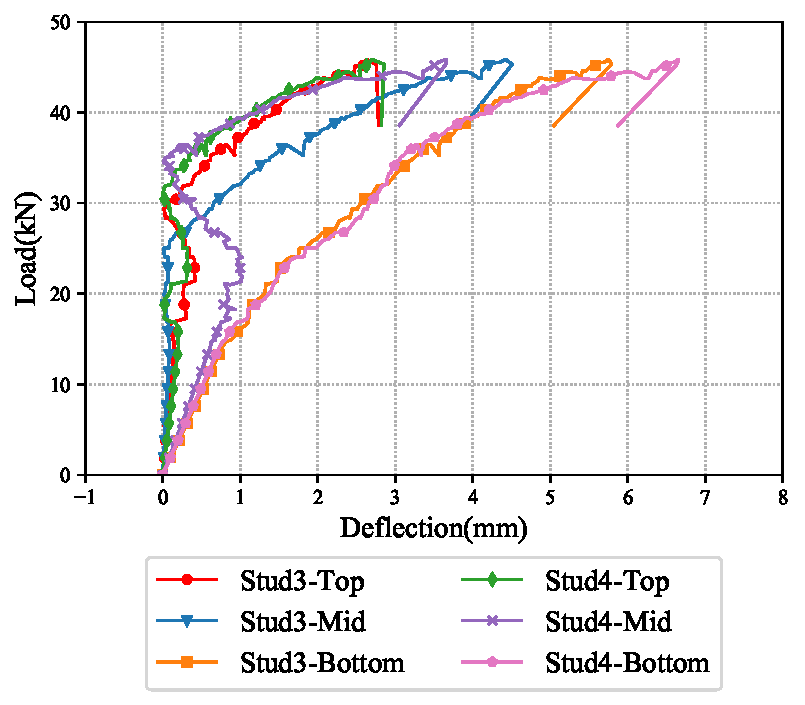
\includegraphics[width=\textwidth]{AT3-Load-Lateral-Corrected.pdf}
		\caption{}
		\label{subfig:AT3-Load-Lateral-Corrected}
	\end{subfigure}
	   \caption{Test-AT3 results - (a) Applied load versus axial displacement and (b) Applied load versus lateral deflection}
	   \label{fig:AT3-results}
\end{figure}

\section{Test-AT4}

The fourth ambient temperature capacity Test-T4 was conducted on double stud LSF wall with 70 mm stud depth. The stud dimensions were 70$\times$29.5$\times$8$\times$0.95 mm (G550 steel). This test was conducted to investigate the ambient temperature capacity of double stud LSF walls with commonly used 70 mm studs. Four studs were used in the test wall and the test configuration is shown in \Cref{fig:AT4-plan}. As a result of bearing failure of edge studs in Test-AT3 the edge studs in Test-AT4 were nested to increase the axial compression loading capacity. The test wall gave an axial compression capacity of 86.21 kN at the end of the test. Significant local buckling of Stud3 of Row-2 in web and flanges was observed as shown in \Cref{fig:AT4-failure} (b). The buckling failure was only observed on Stud3 of Row-1. A large crack was observed on the plasterboard at the stud failure location as shown in \Cref{fig:AT4-failure} (a).
\begin{figure}[!htbp]
	\centering
			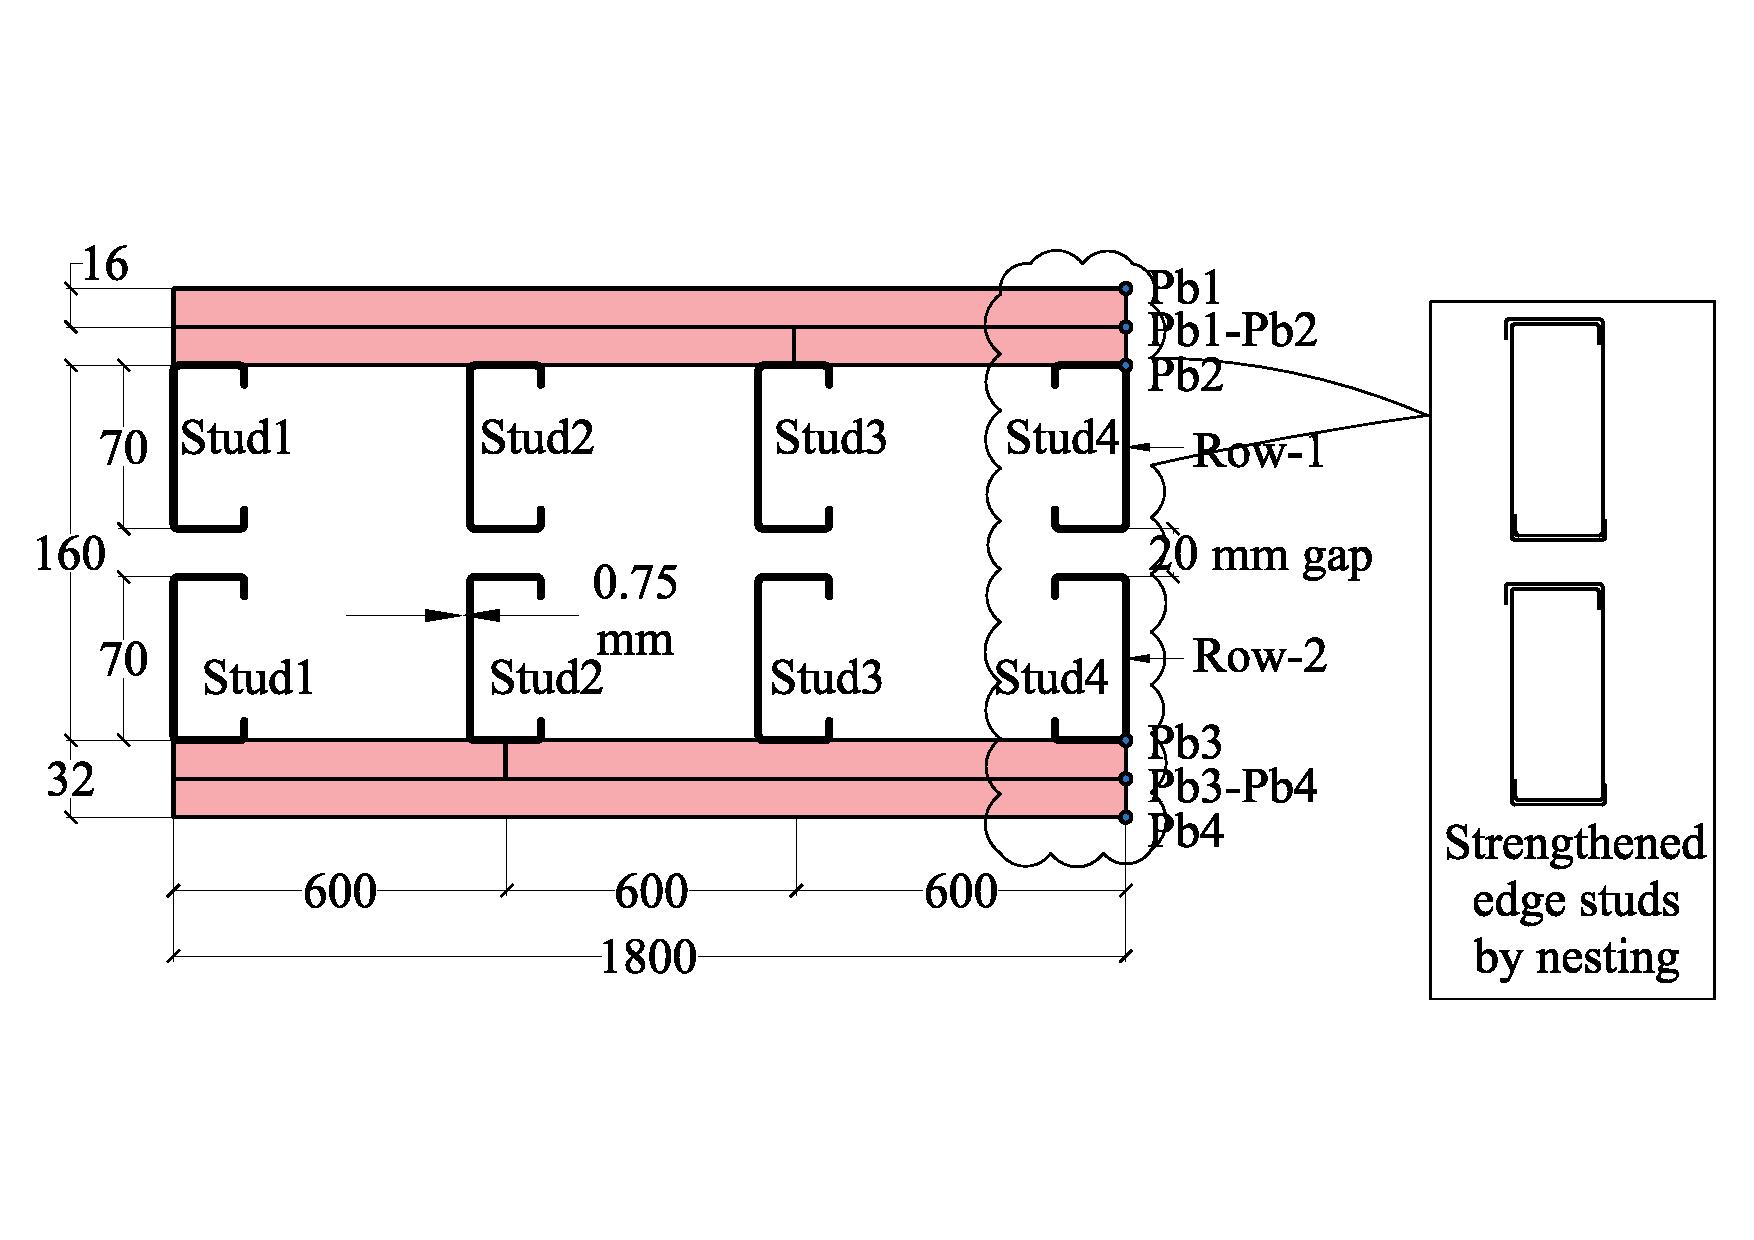
\includegraphics[scale=0.25]{AT4-plan.pdf}\\
		\caption{Test-AT4 configuration}
		\label{fig:AT4-plan}
\end{figure}  
\begin{figure}[!htbp]
	\centering
	\begin{subfigure}[b]{0.3\textwidth}
		\centering
		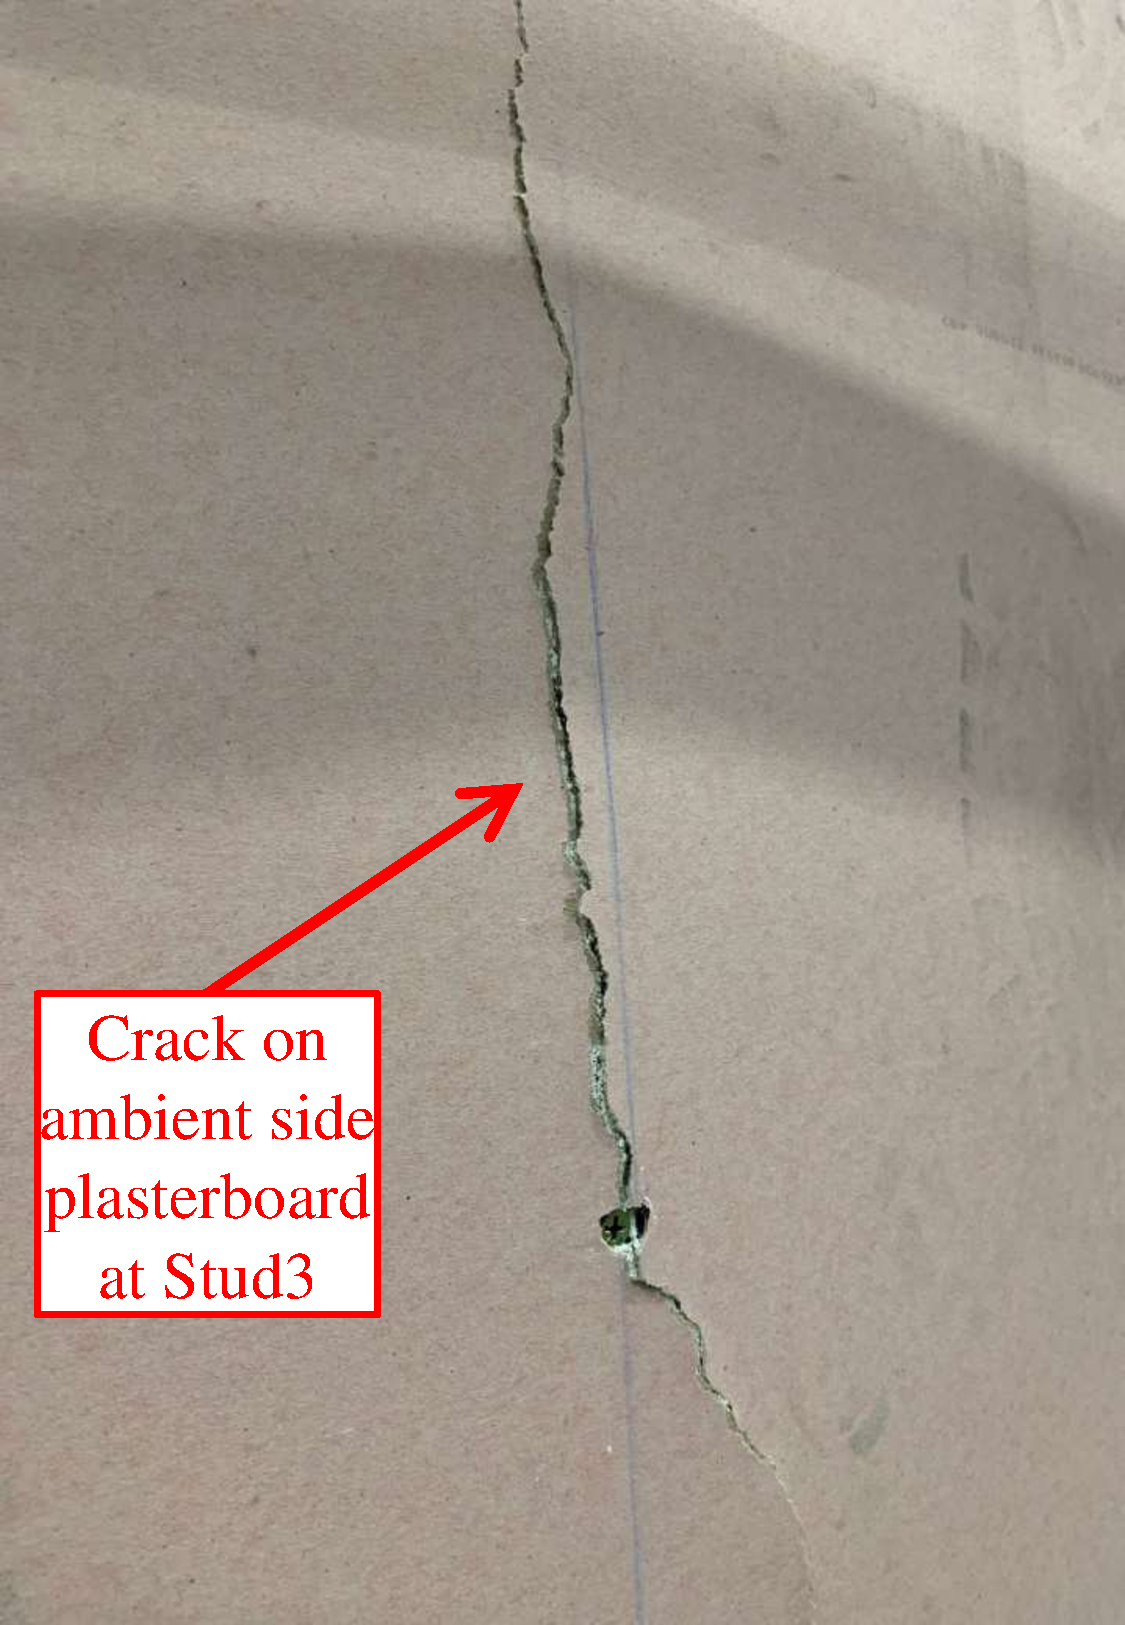
\includegraphics[width=\textwidth]{AT4-plasterboard_crack.pdf}
		\caption{}
		\label{subfig:AT4-plasterboard_crack}
	\end{subfigure}
	\begin{subfigure}[b]{0.3\textwidth}
		\centering
		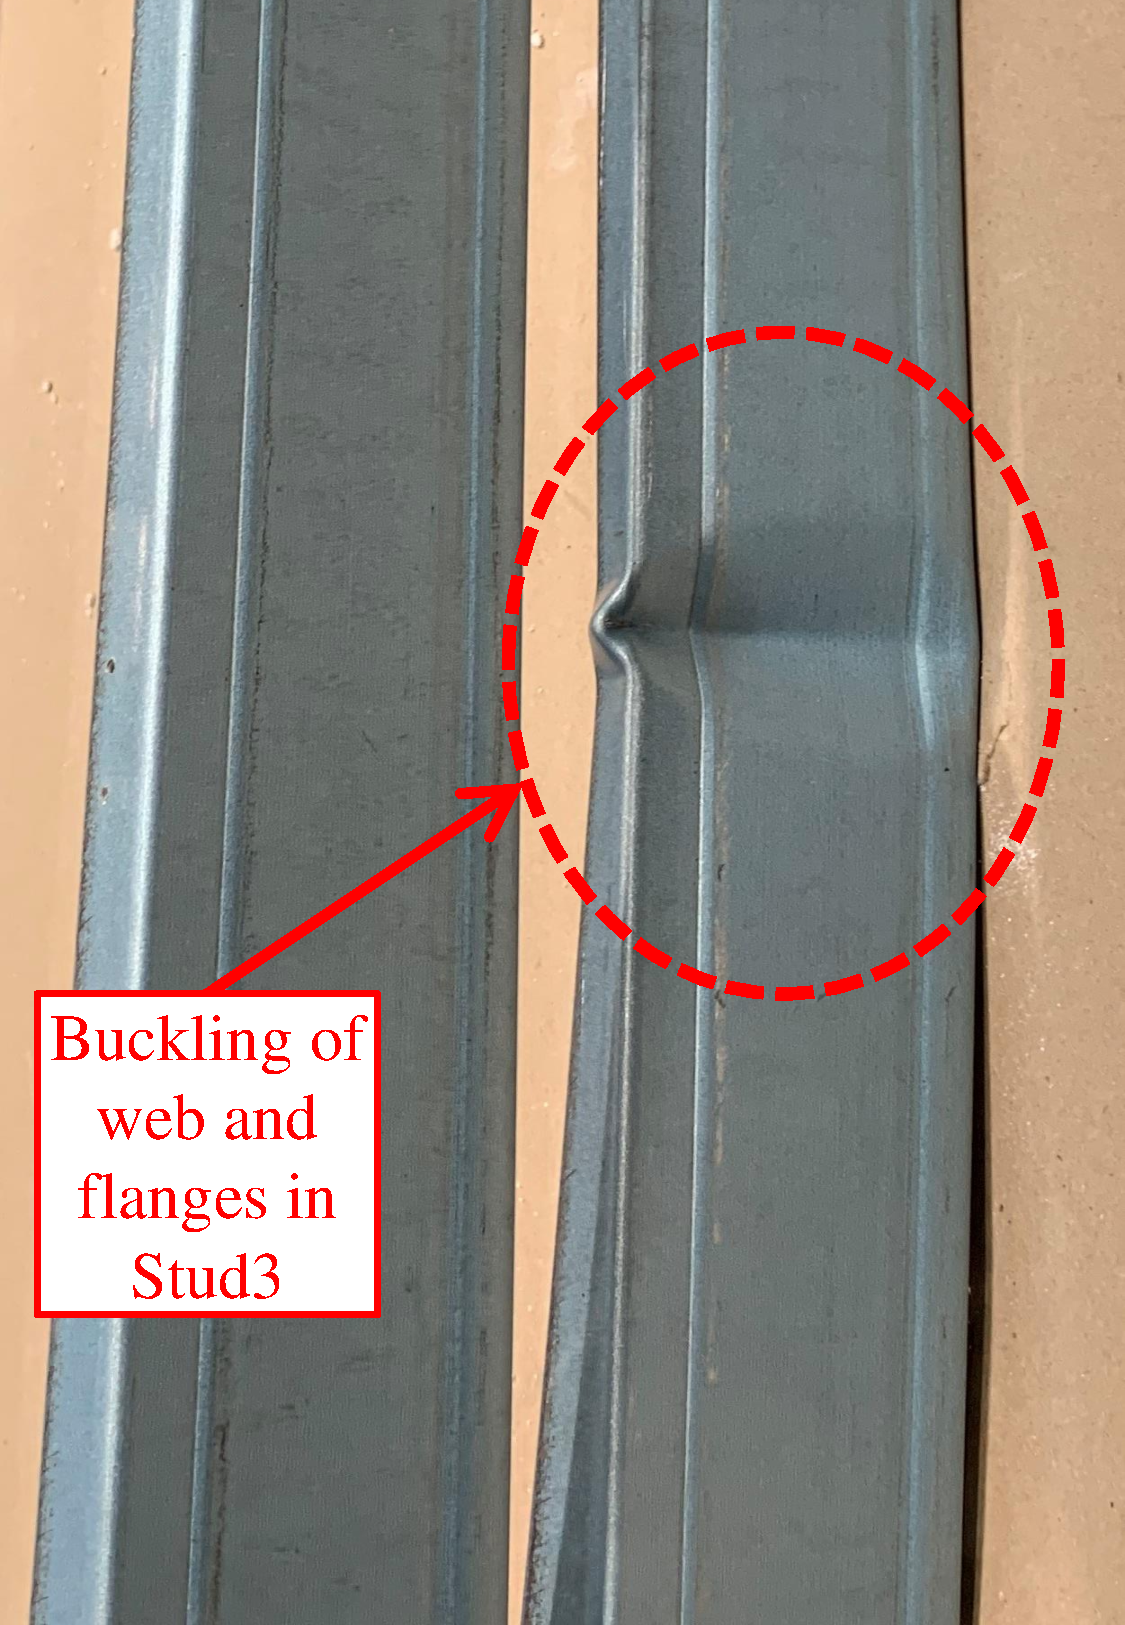
\includegraphics[width=\textwidth]{AT4-buckling.pdf}
		\caption{}
		\label{subfig:AT4-buckling}
	\end{subfigure}
	   \caption{Test-AT4 results - (a) Plasterboard crack and (b) Buckling of stud}
	   \label{fig:AT4-failure}
\end{figure}
\begin{figure}[!htbp]
	\centering
	\begin{subfigure}[b]{0.7\textwidth}
		\centering
		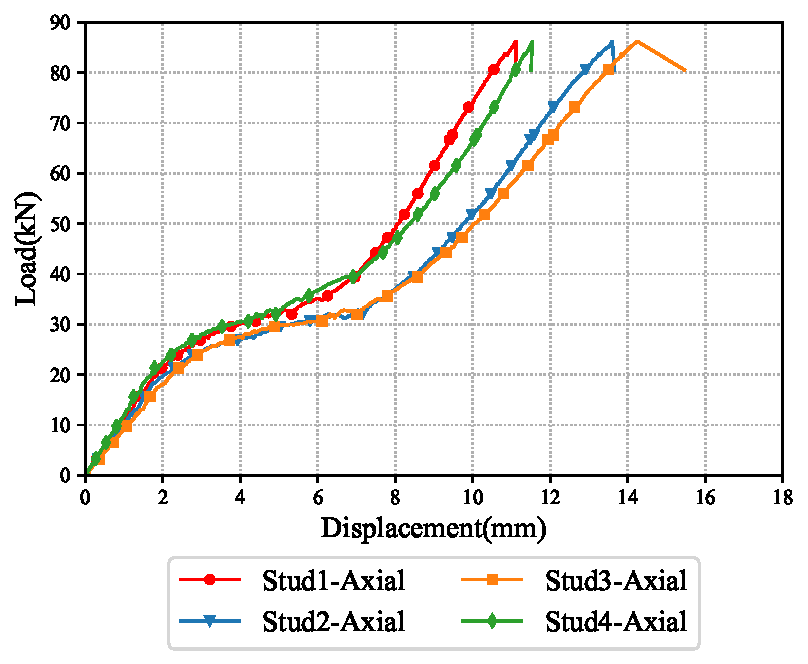
\includegraphics[width=\textwidth]{AT4-Load-Axial-Corrected.pdf}
		\caption{}
		\label{subfig:AT4-Load-Axial-Corrected}
	\end{subfigure}
	\begin{subfigure}[b]{0.7\textwidth}
		\centering
		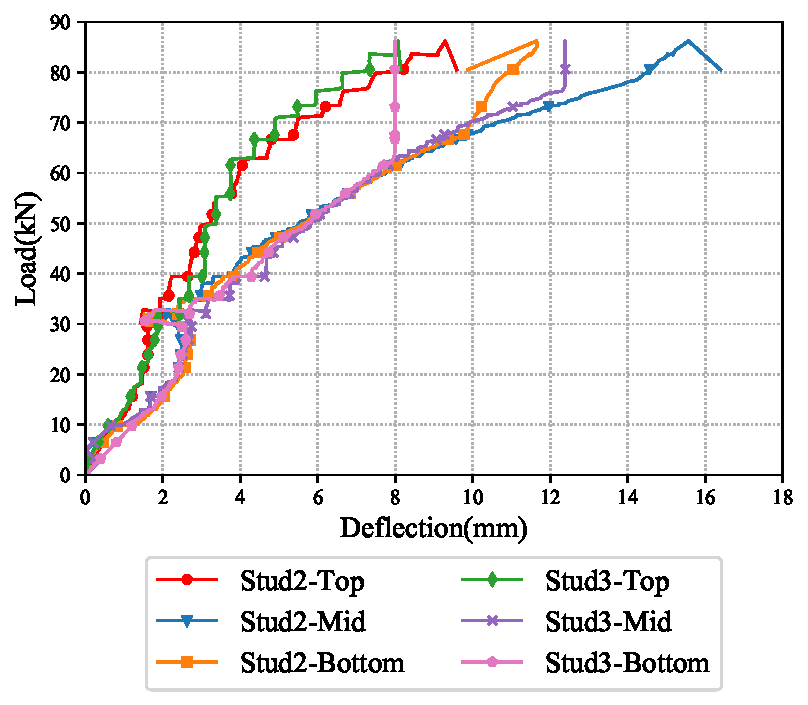
\includegraphics[width=\textwidth]{AT4-Load-Lateral-Corrected.pdf}
		\caption{}
		\label{subfig:AT4-Load-Lateral-Corrected}
	\end{subfigure}
	   \caption{Test-AT4 results - (a) Applied load versus axial displacement and (b) Applied load versus lateral deflection}
	   \label{fig:AT4-results}
\end{figure}

The applied axial load versus the axial displacement and lateral deflection curves of Test-AT4 are shown in Figures \ref{fig:AT4-results} (a) and (b). Maximum axial displacement of 15.46 mm was recorded for Stud3. This indicates the structural failure of Stud3 of Row-2 as shown in \Cref{fig:AT4-failure} (b). The maximum lateral deflection was 16.39 mm at Stud2-Mid (1500 mm) indicating the out-of plane deflection in the test wall. Comparison with the ambient temperature capacity of Test-T1 revealed that the axial compression capacity increased by 13.21 kN (86.21-73 kN) in comparison with Tests-AT1 with the same thickness of 0.95 mm. This increase in axial compression capacity would have been attributed to several factors such as the geometric dimensions and slenderness ratios of the studs. It is to note that the flanges are 1 mm longer in the 70 mm deep studs in comparison with the 90 mm deep studs as shown in Figures \ref{fig:stud-cross-section} (a) and (b). Also, the maximum slenderness ratio (b/t) of the studs used in Test-T1 is 94.73 ($90/0.95$) while it is 73.68 ($70/0.95$) for Test-T4 if the local buckling of the web is considered. Hence Test-T4 gave an increased axial compression capacity. 

\section{Test-AT5}

The last ambient temperature capacity test was conducted on a staggered stud LSF wall. The test wall consisted of two rows of studs positioned in a staggered manner. The studs were 90$\times$36$\times$7$\times$0.95 mm (G550 steel). Eleven studs were used in the staggered configuration as shown in \Cref{fig:AT5-plan}. 
\begin{figure}[!htbp]
	\centering
			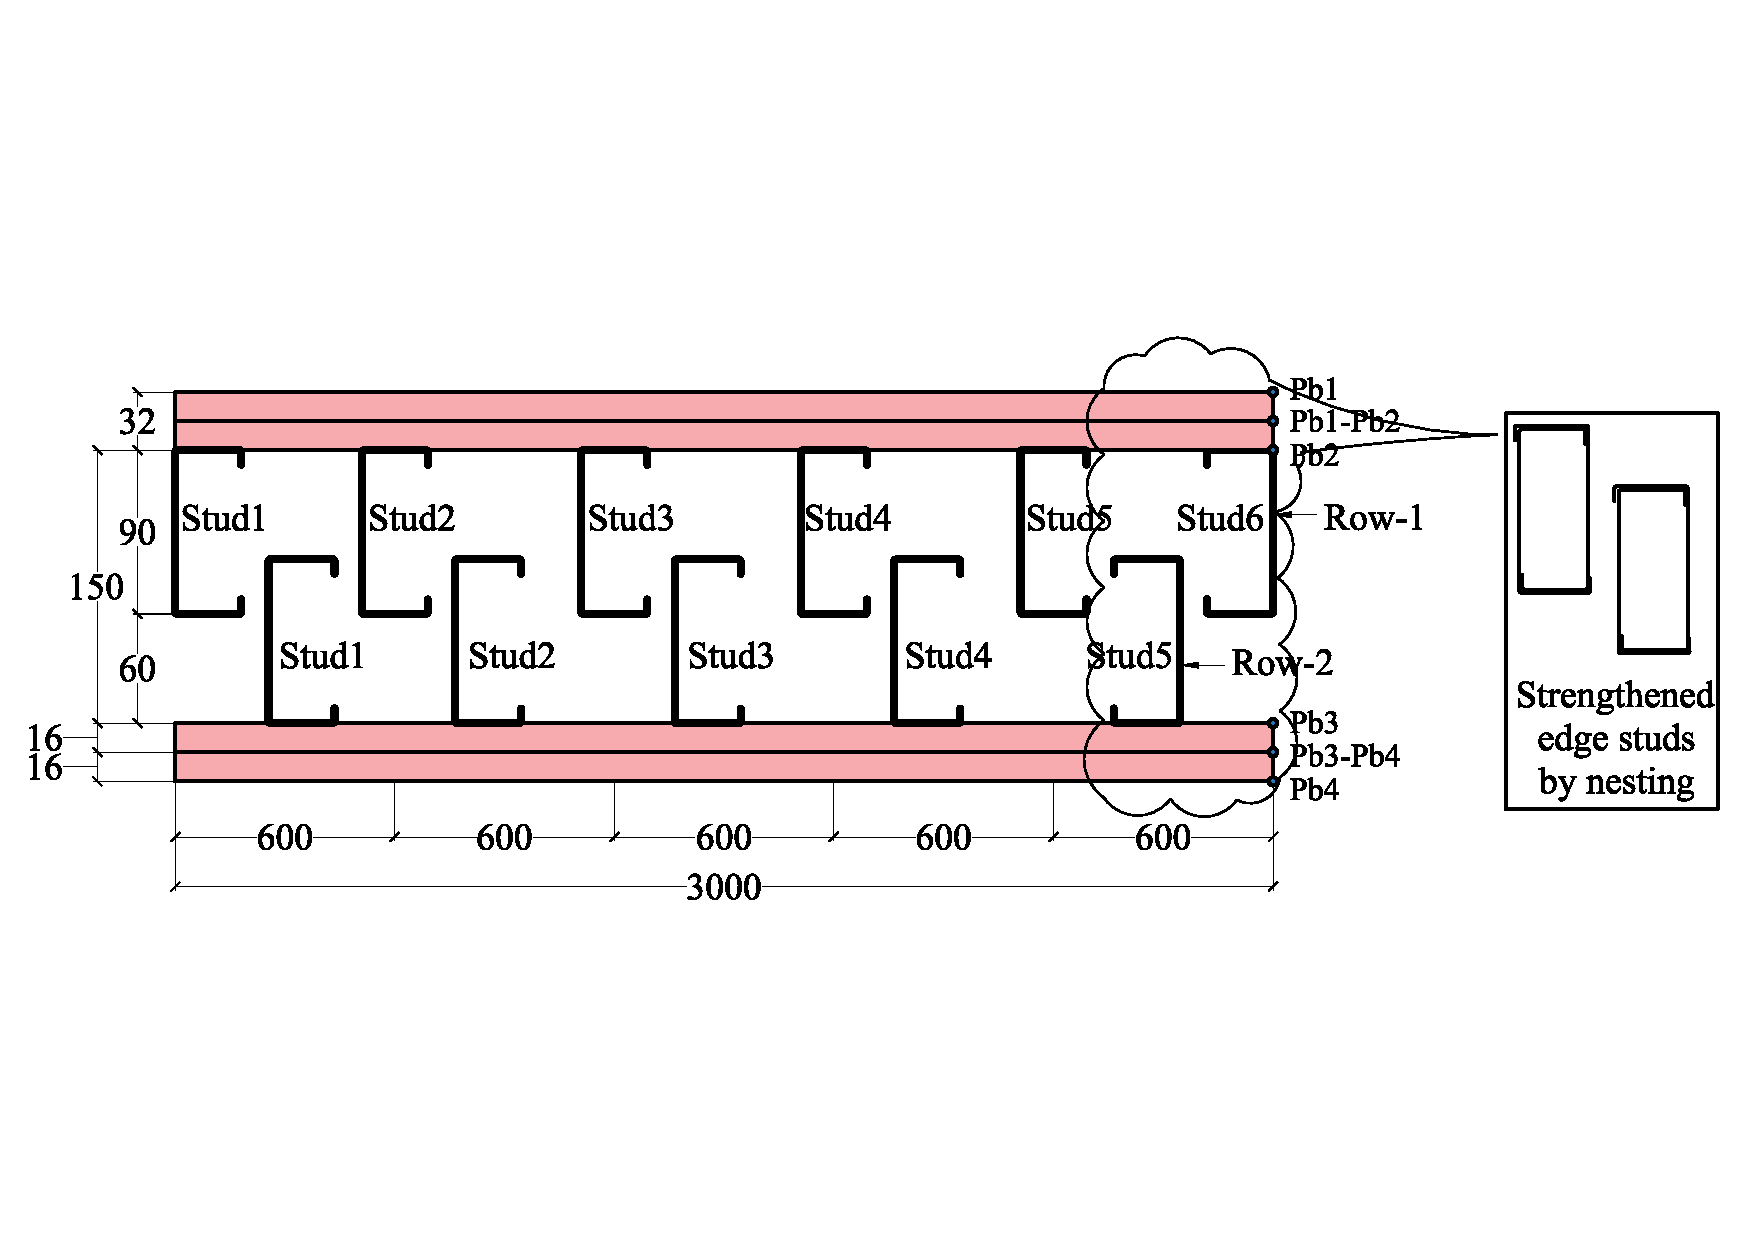
\includegraphics[scale=0.35]{AT5-plan.pdf}\\
		\caption{Test-AT5 configuration}
		\label{fig:AT5-plan}
\end{figure}

Edge studs were nested to avoid bearing failure of studs in the test wall. Previous ambient temperature capacity tests (AT1-AT4) had UCS noggings connecting the flanges and provided lateral restraints at 1 m intervals against minor axis buckling. However, in a staggered stud wall, the discontinuity between the stud rows is necessary to achieve the required acoustic rating. Therefore, omega noggings rails were used at 1 m intervals to provide the required lateral restraints to the studs. As the name suggests, the omega nogging rails are shaped as the greek symbol omega ($\Omega$). The omega noggings are connected to every alternate studs on the stud webs at service holes through a connecting clip. Details of the omega nogging and the connecting clip are shown in Figures \ref{fig:Omega-nogging-connections} (a) and (b). The clips are held on to web at one end and snapped on to the groves of the omega nogging at two locations. The nogging to stud connection details are shown in \Cref{fig:AT5-construction} (a). Unlike other tests, the stud to track connection needed additional components. As the arrangement of the studs are staggered, the tracks are connected to only one flange of the stud. Hence an end cleat was used between the unsupported flange and the track as shown in \Cref{fig:Omega-nogging-connections} (c). The end cleats were manufactured in-house at QUT Wind and Fire Engineering Laboratory and were made with one lip longer than the other. The longer lip of the cleat was attached to the unrestrained stud flanges while the shorter lip was attached to the tracks' lip using two D-Type 16 mm screws. End cleats were used in the stud to track connections to improve their fixity conditions in the ambient capacity test as shown in \Cref{fig:AT5-construction} (b). 
\begin{figure}[!htbp]
	\centering
		\begin{tabular}{ccc}
			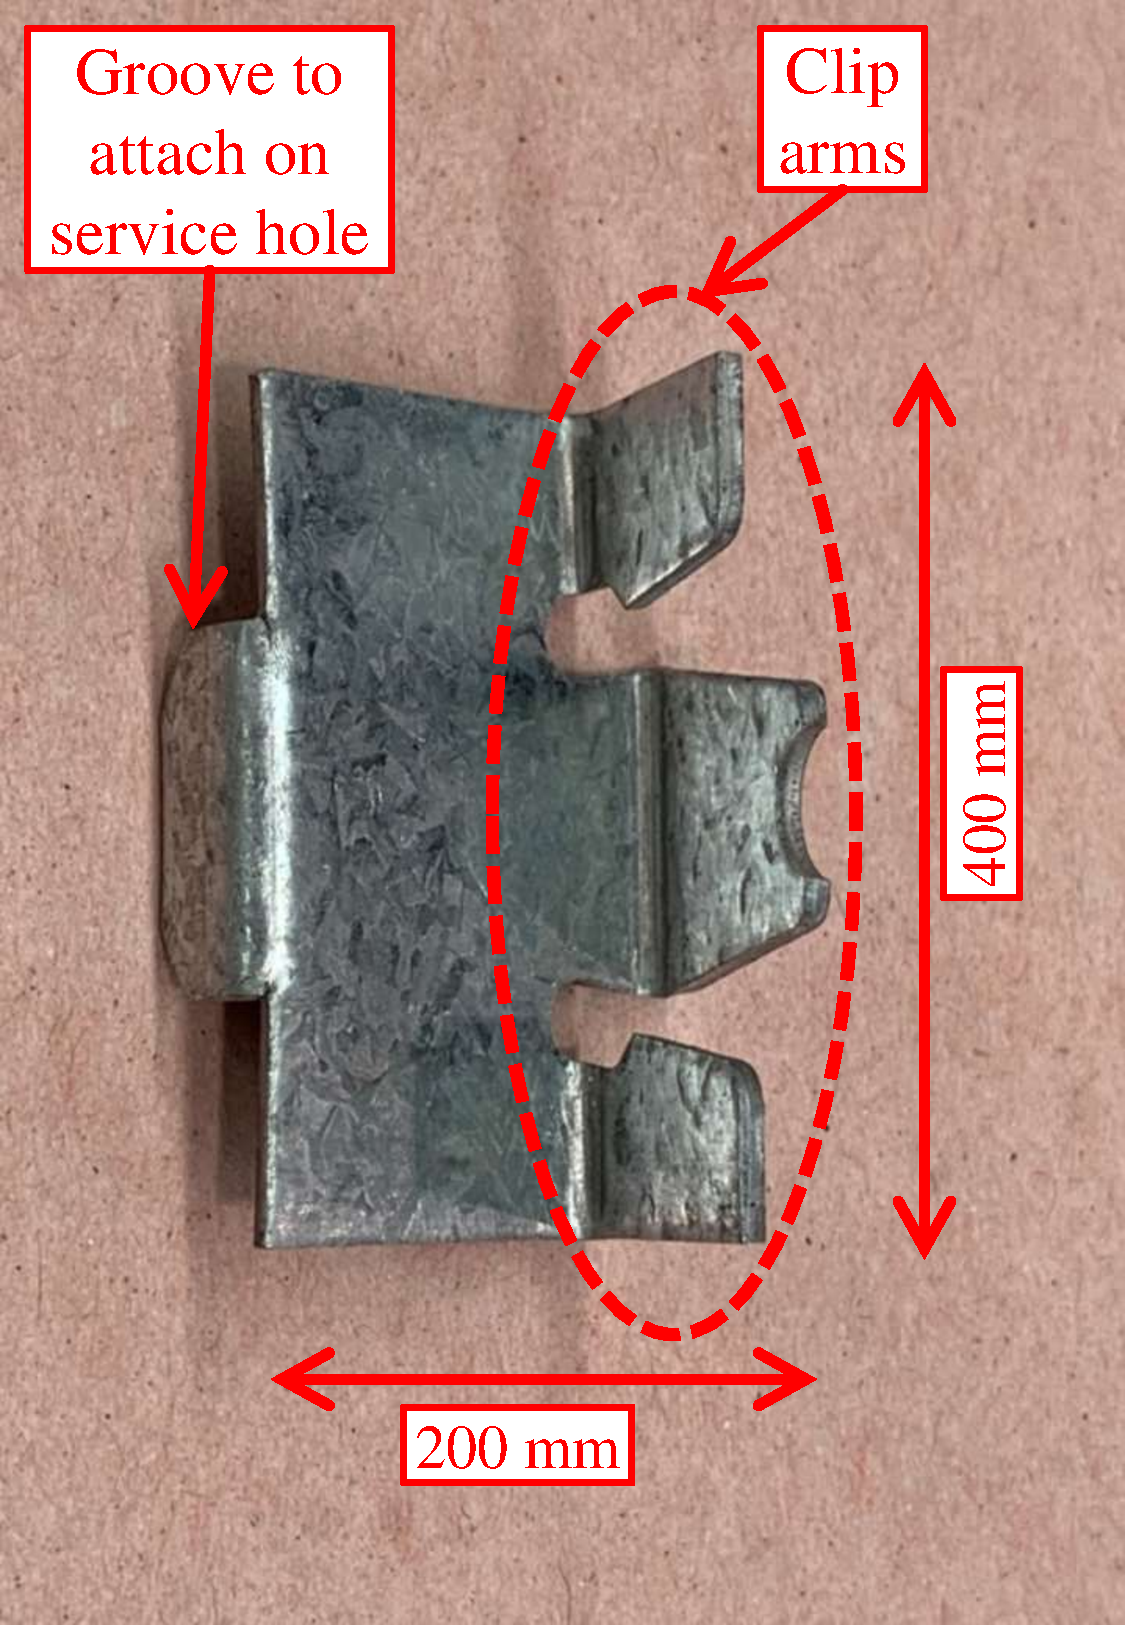
\includegraphics[width=4.25cm,height=6cm]{omega-nogging-clip.pdf} & 
			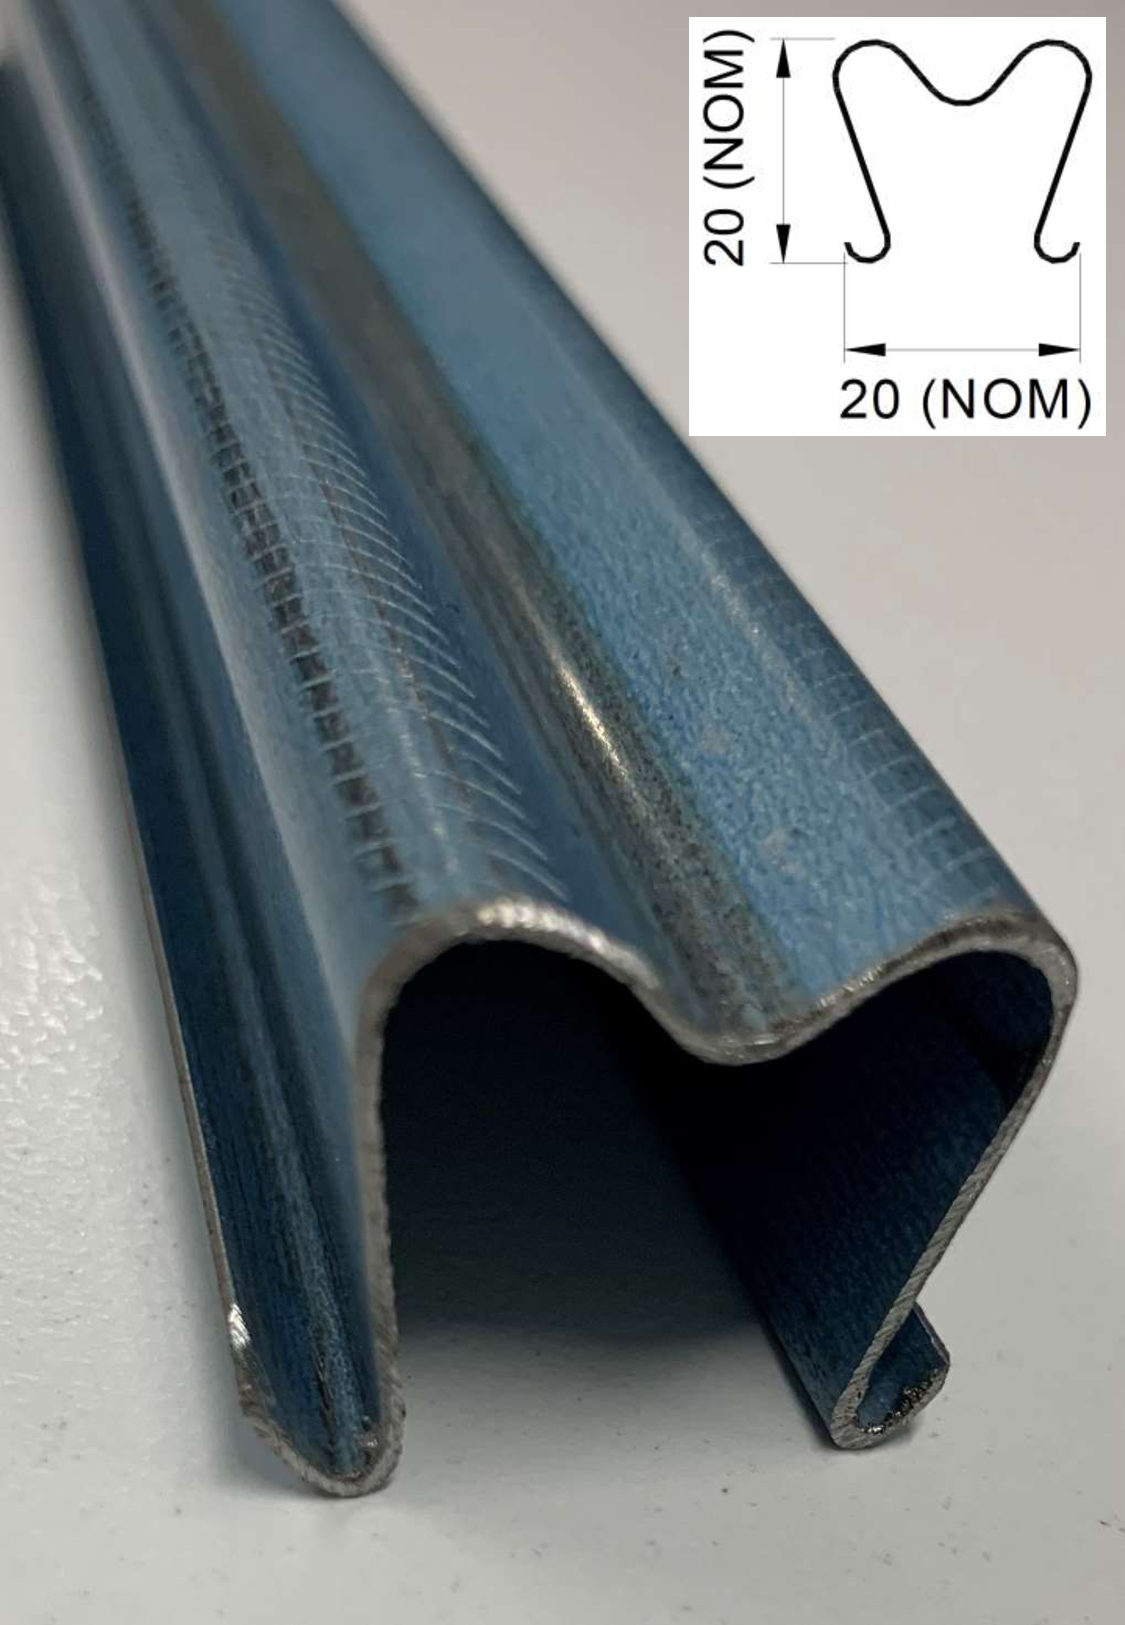
\includegraphics[width=4.25cm,height=6cm]{omega-nogging-rail.pdf} & 
			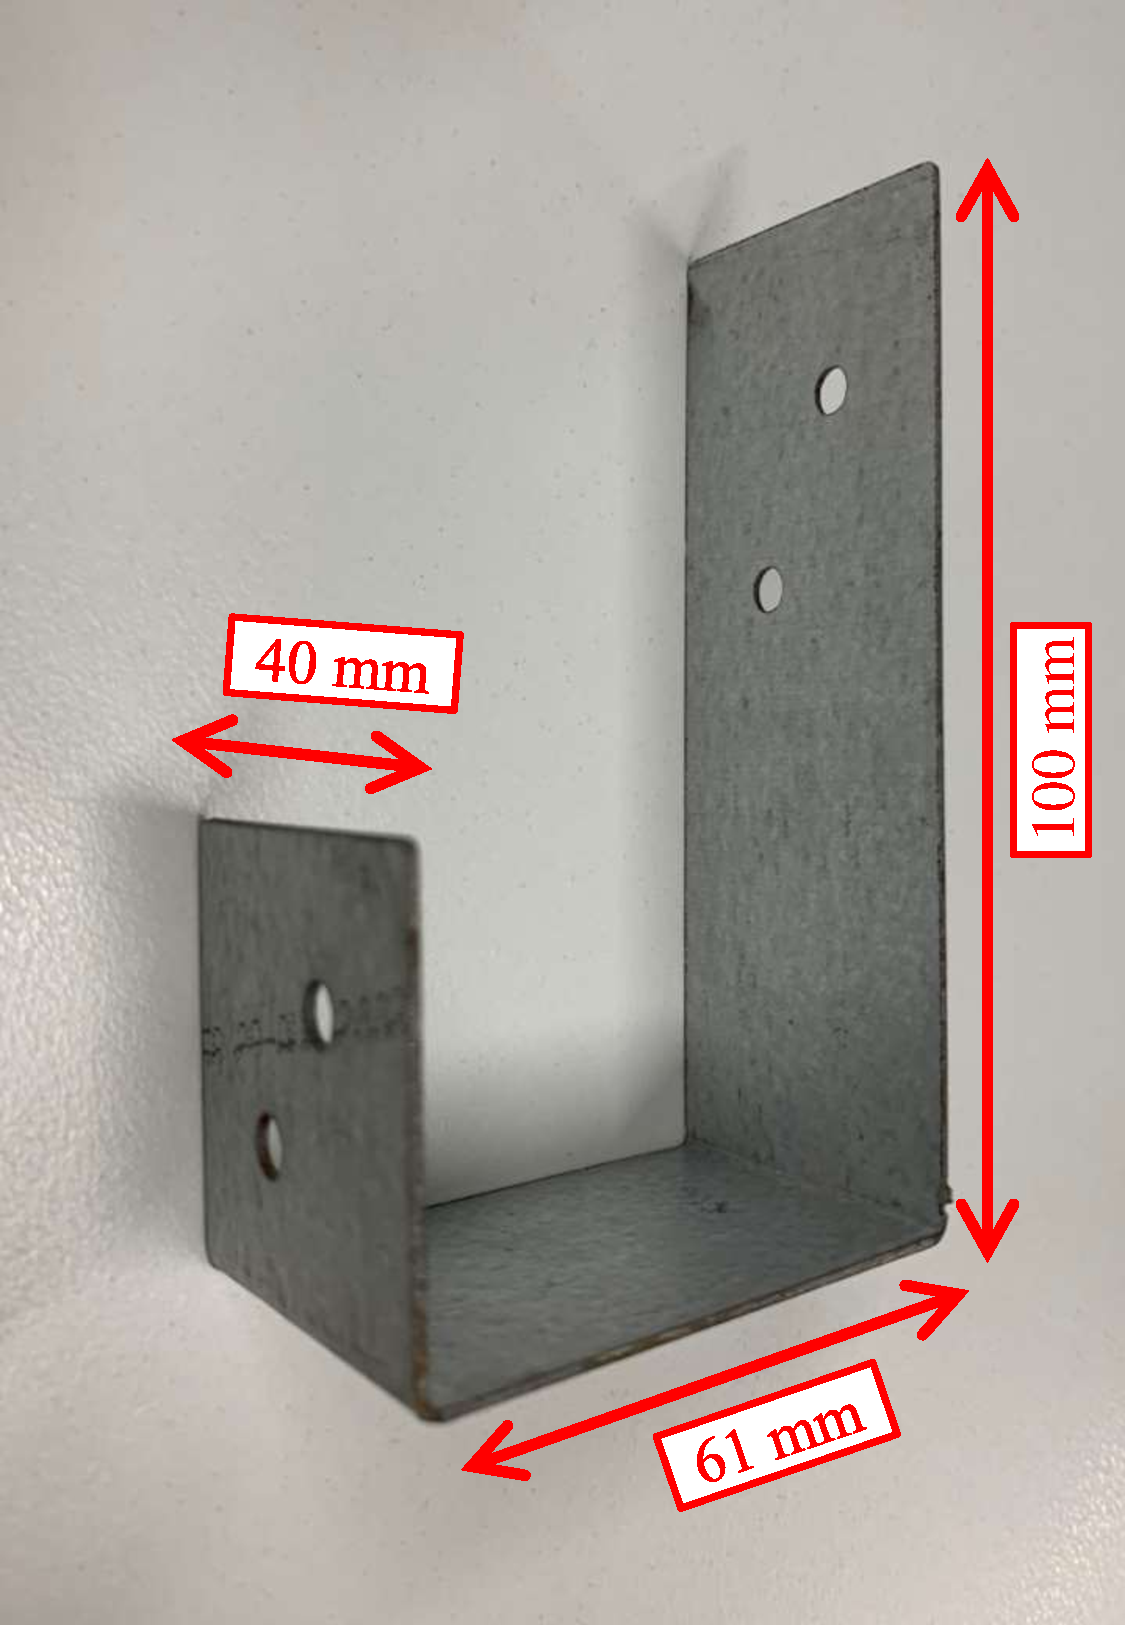
\includegraphics[width=4.25cm,height=6cm]{staggered-cleat.pdf} \\
			(a) & (b) & (c) \\ 
		\end{tabular} 
		\caption{Test-AT5 wall components - (a) Omega nogging clip (b) Omega nogging rail (c) End cleat}
		\label{fig:Omega-nogging-connections}
\end{figure}
\begin{figure}[!htbp]
	\centering
	\begin{subfigure}[b]{0.5\textwidth}
		\centering
		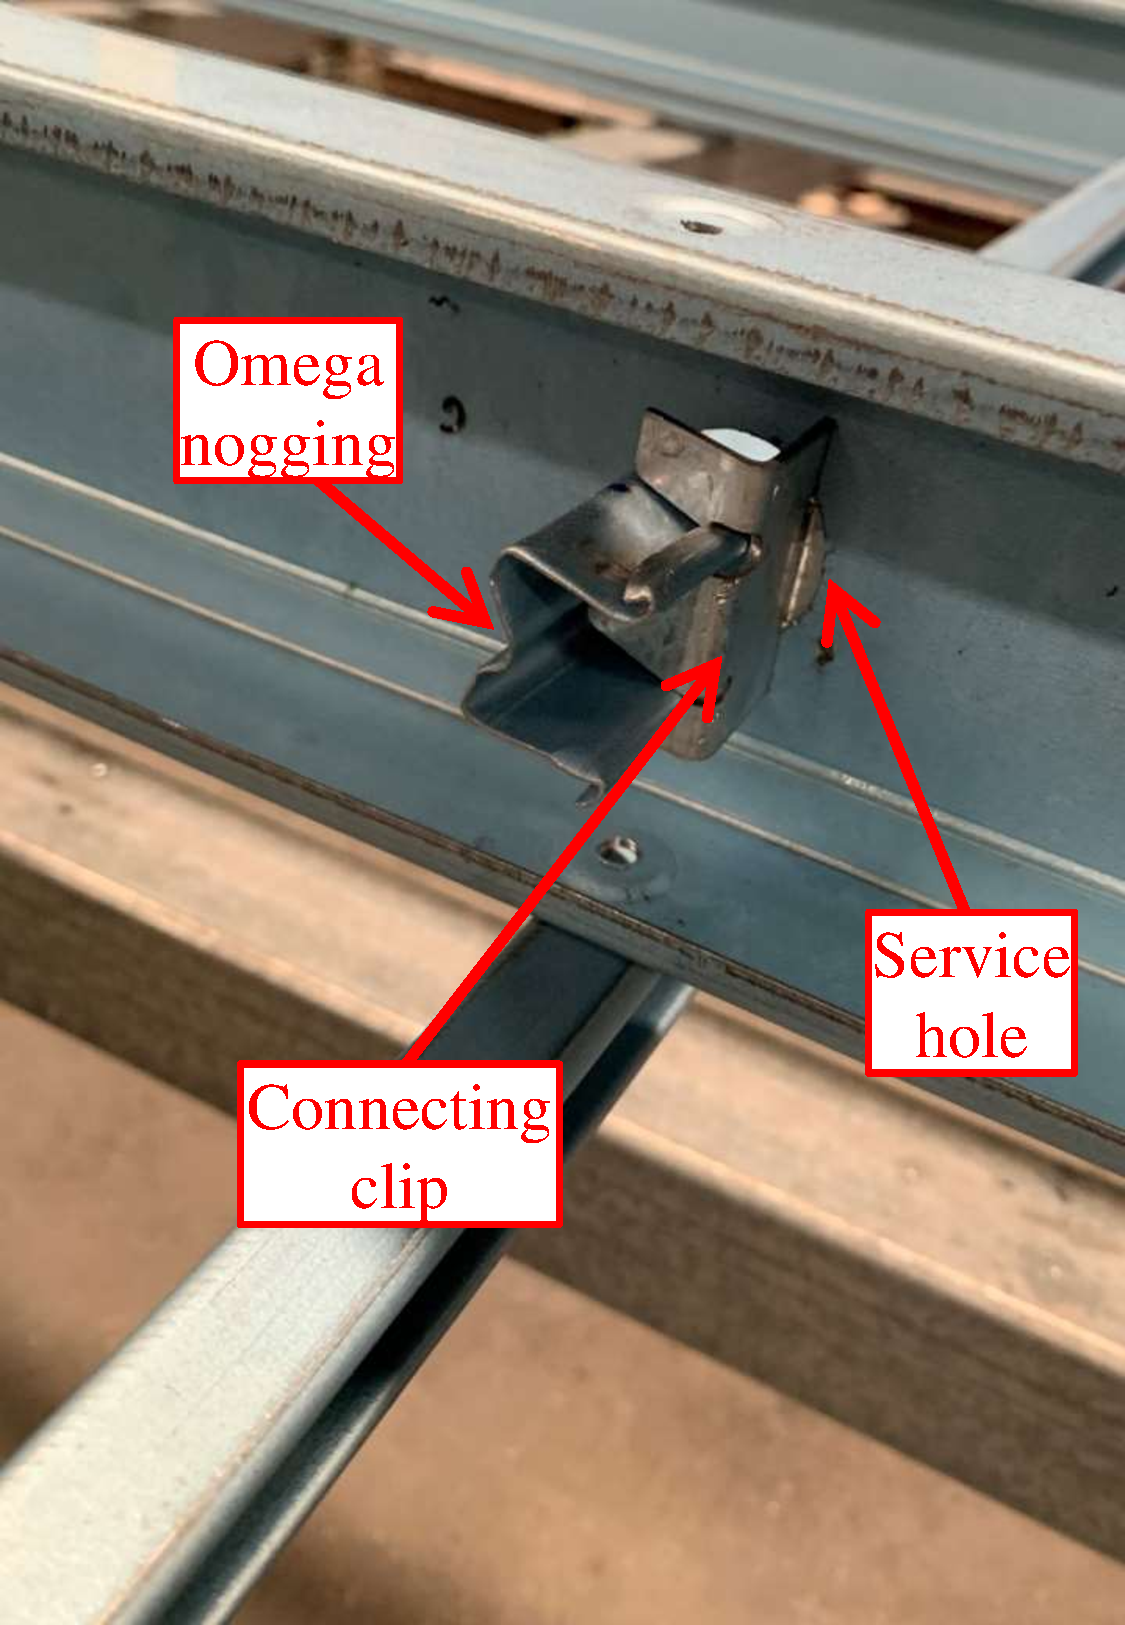
\includegraphics[width=\textwidth]{omega_connection.pdf}
		\caption{}
		\label{subfig:omega_connection}
	\end{subfigure}
	\begin{subfigure}[b]{0.8\textwidth}
		\centering
		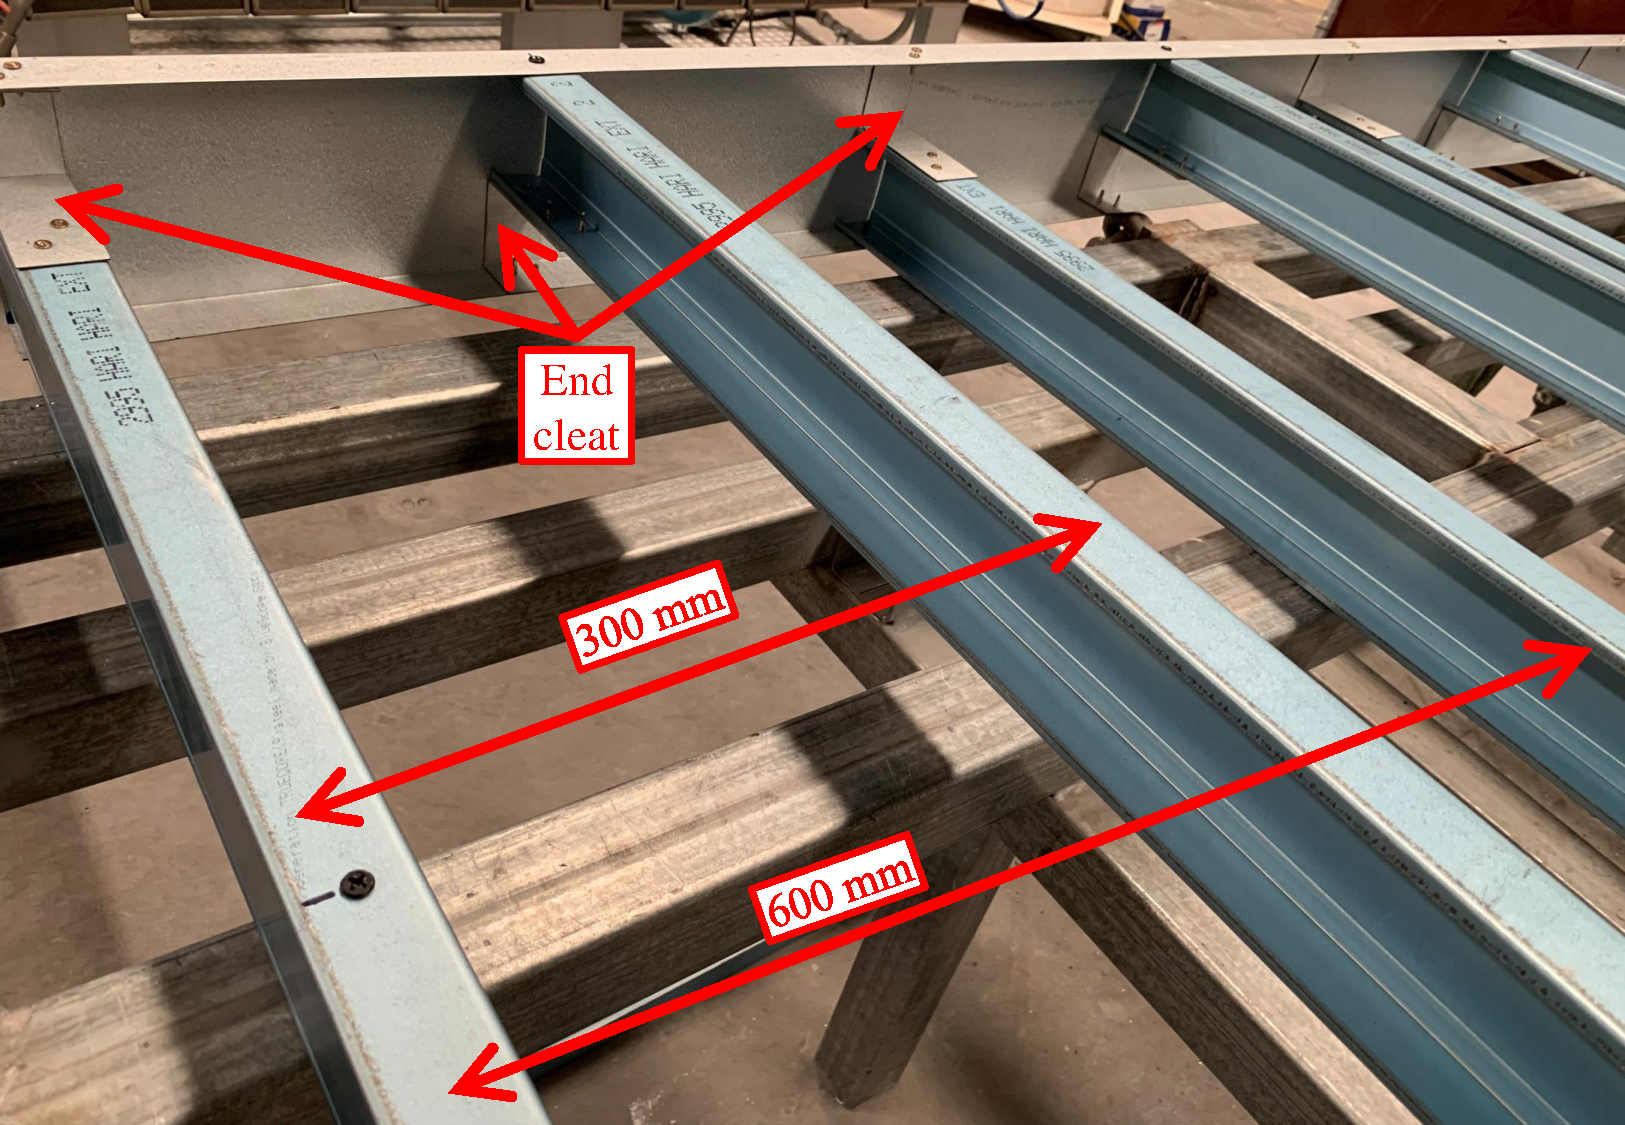
\includegraphics[width=\textwidth]{AT5-construction.pdf}
		\caption{}
		\label{subfig:AT5-wall-construction}
	\end{subfigure}
	   \caption{Test-AT5 wall construction- (a) Omega nogging and clip connection (b) Staggered stud wall construction}
	   \label{fig:AT5-construction}
\end{figure}
\begin{figure}[!htbp]
	\centering
	\begin{subfigure}[b]{0.4\textwidth}
		\centering
		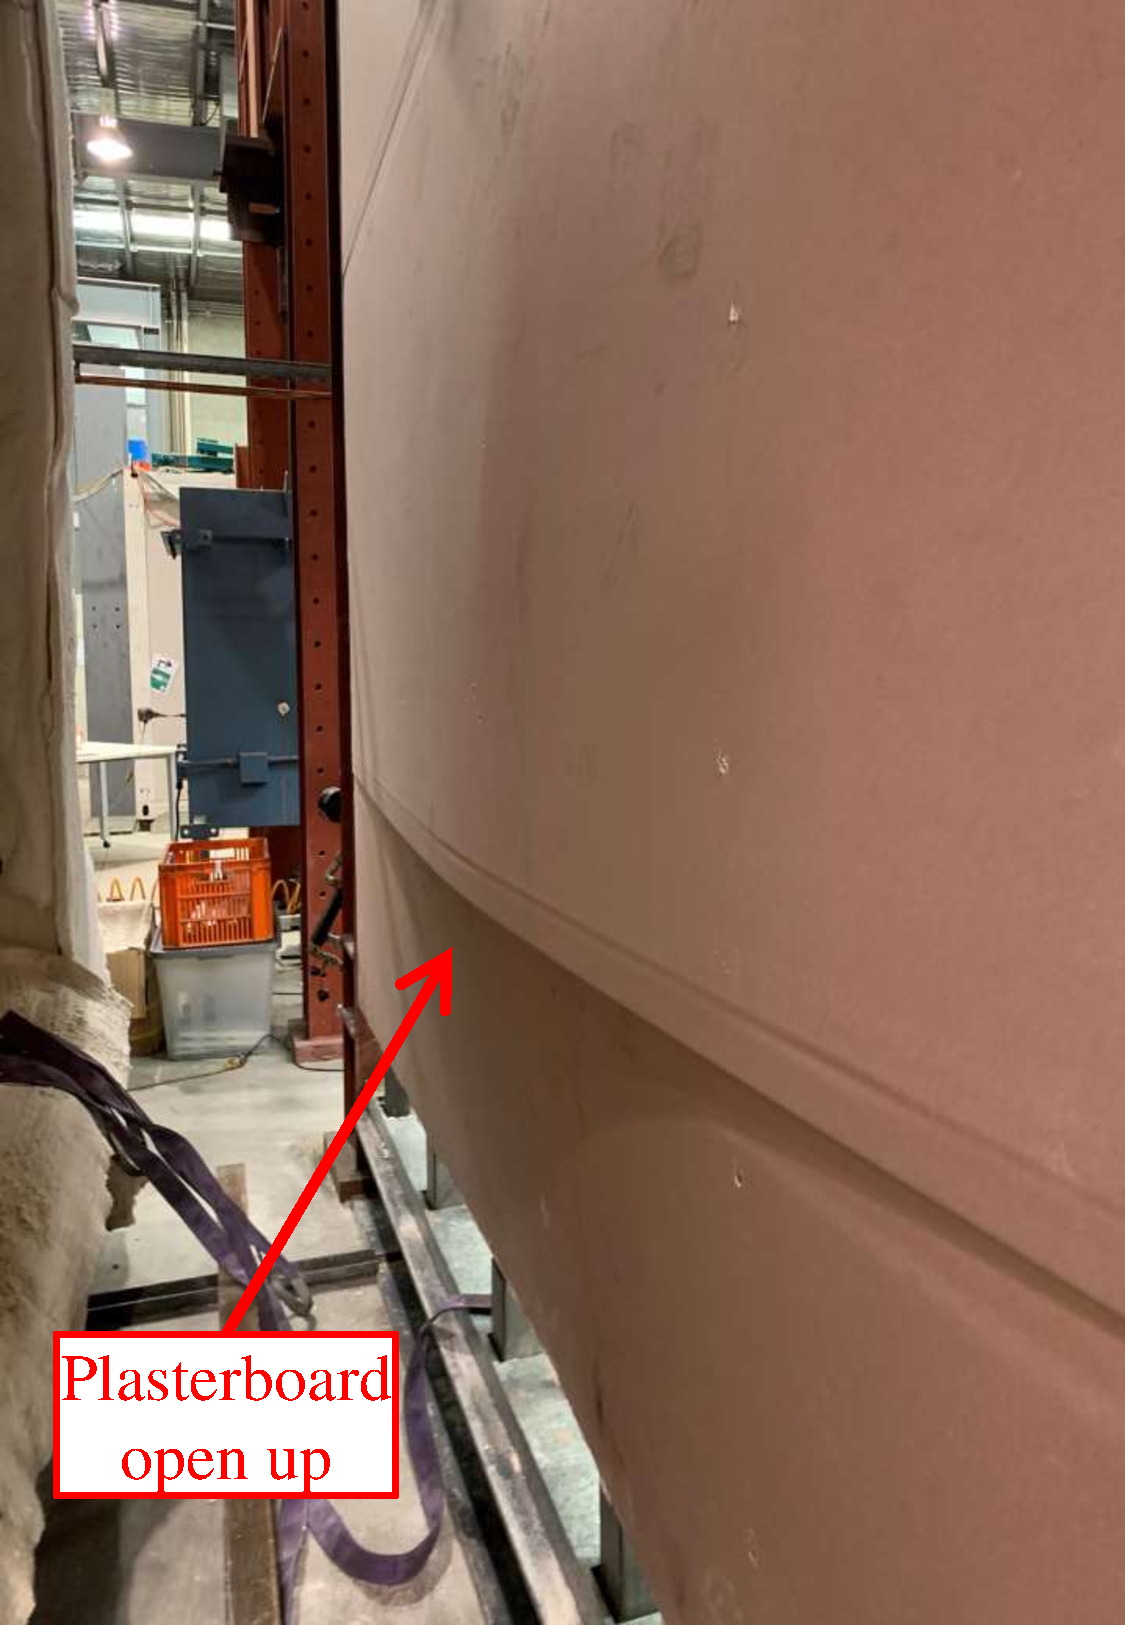
\includegraphics[width=\textwidth]{AT5-plasterboard.pdf}
		\caption{}
		\label{subfig:AT5-full-buckling}
	\end{subfigure}
	\begin{subfigure}[b]{0.5\textwidth}
		\centering
		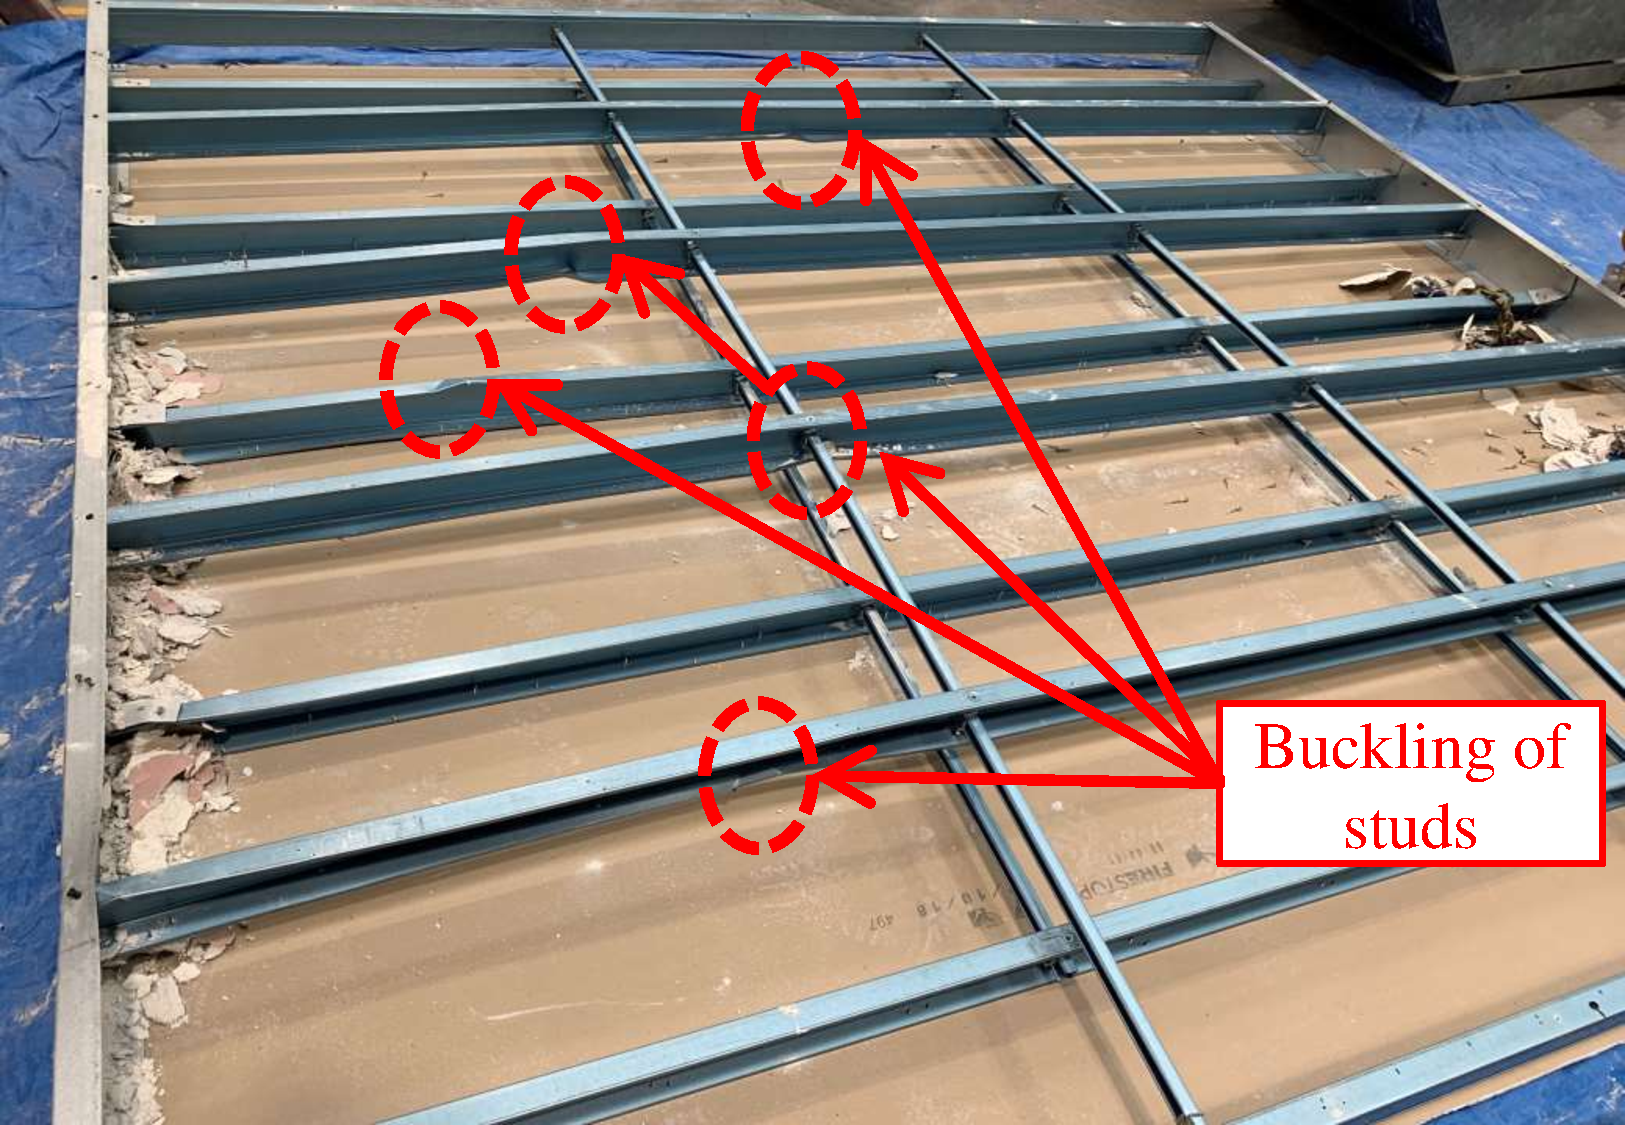
\includegraphics[width=\textwidth]{AT5-full-buckling.pdf}
		\caption{}
		\label{subfig:AT5-plasterboard}
	\end{subfigure}
	\begin{subfigure}[b]{0.45\textwidth}
		\centering
		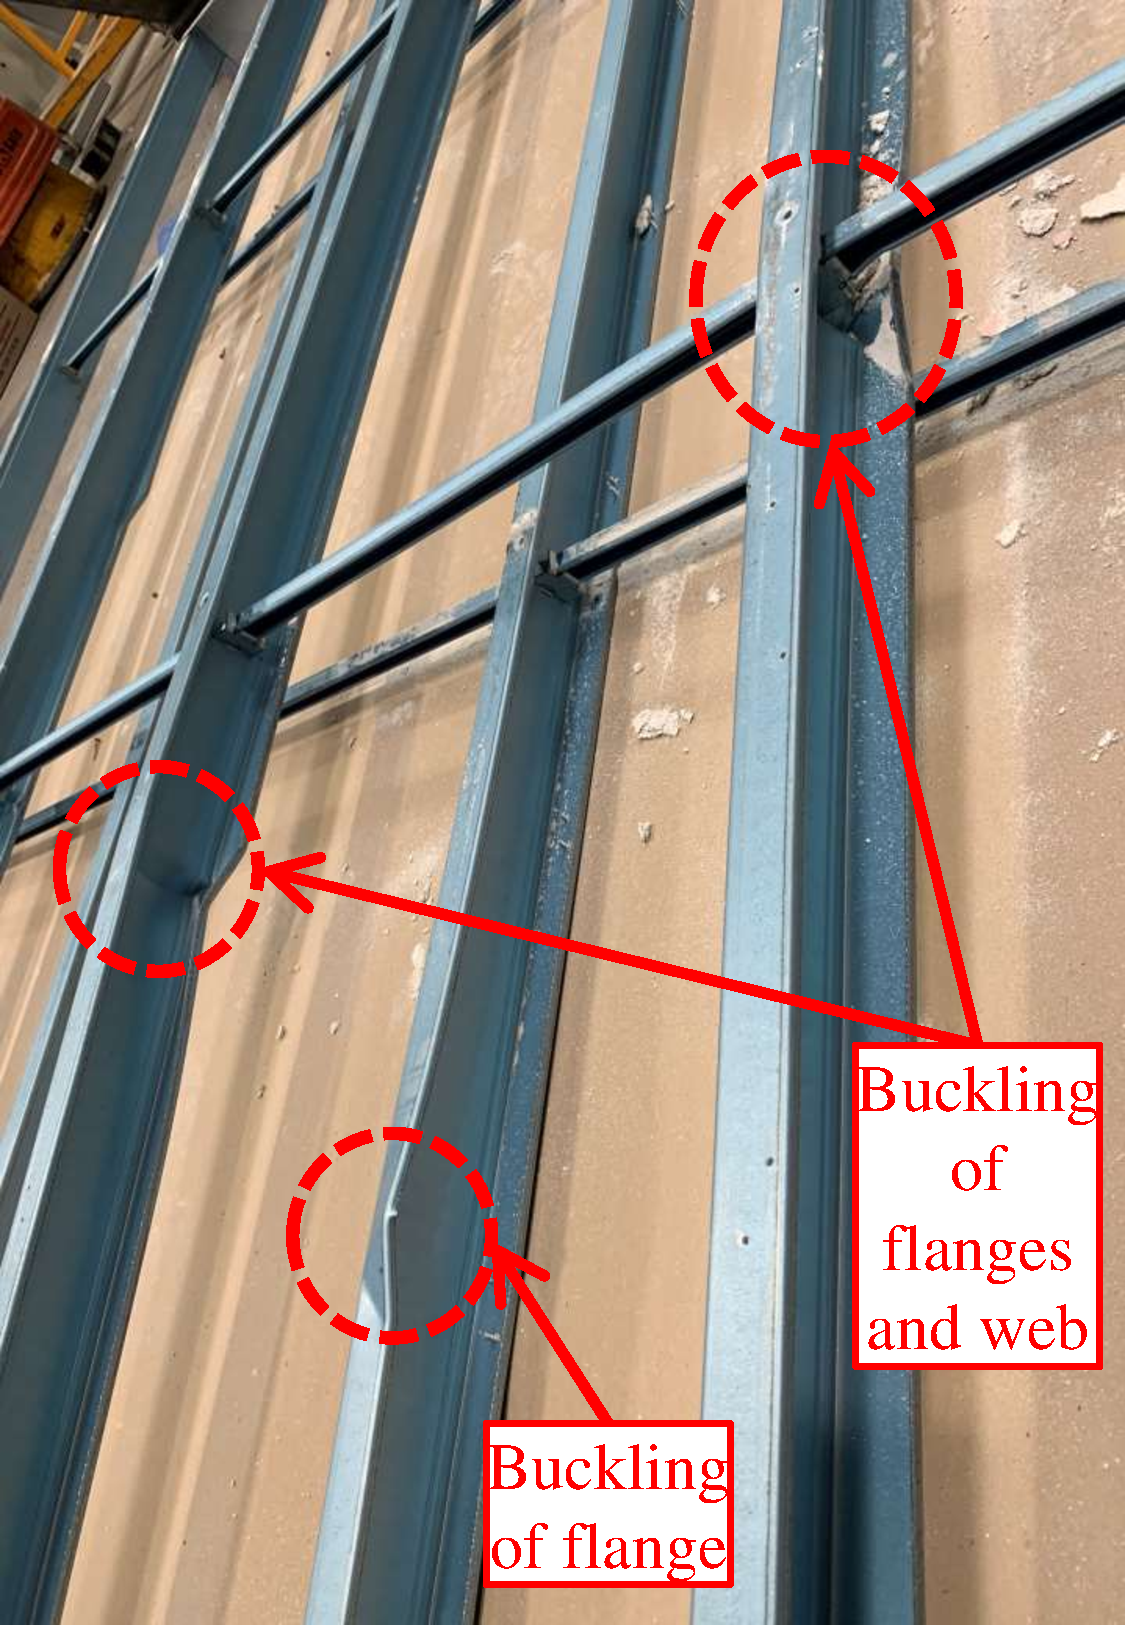
\includegraphics[width=\textwidth]{AT5-buckling.pdf}
		\caption{}
		\label{subfig:AT5-buckling}
	\end{subfigure}
	   \caption{Test-AT5 - failure (a) Plasterboard open up  (b) Buckling of studs in test wall (c) Buckling of studs - close up }
	   \label{fig:AT5-failure}
\end{figure}
\begin{figure}[!htbp]
	\centering
	\begin{subfigure}[b]{0.7\textwidth}
		\centering
		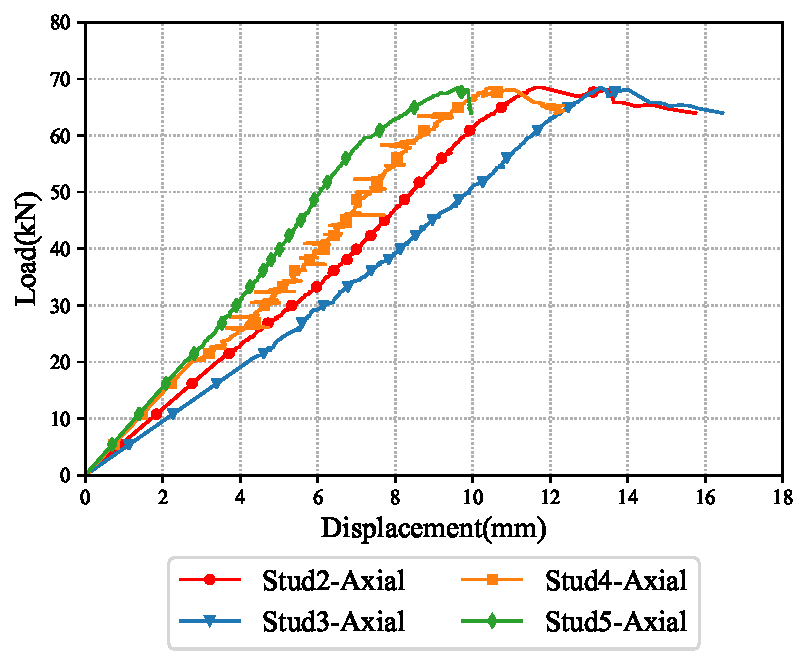
\includegraphics[width=\textwidth]{AT5-Load-Axial-Corrected.pdf}
		\caption{}
		\label{subfig:AT5-Load-Axial-Corrected}
	\end{subfigure}
	\begin{subfigure}[b]{0.7\textwidth}
		\centering
		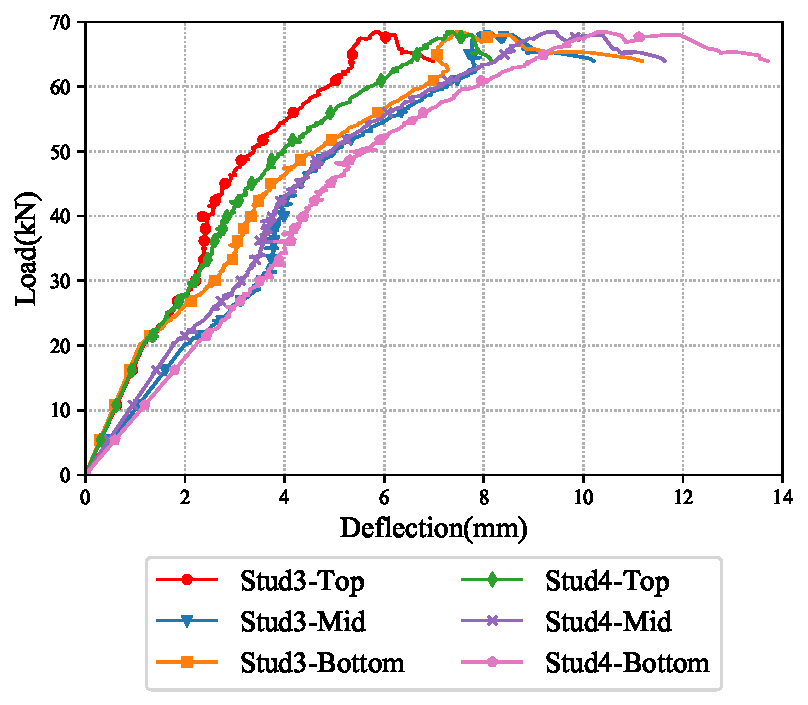
\includegraphics[width=\textwidth]{AT5-Load-Lateral-Corrected.pdf}
		\caption{}
		\label{subfig:AT5-Load-Lateral-Corrected}
	\end{subfigure}
	   \caption{Test-AT5 results - (a) Applied load versus axial displacement and (b) Applied load versus lateral deflection}
	   \label{fig:AT5-results}
\end{figure}

The test wall was loaded through a 20 mm thick base plate connecting the rams and the axial compression load was applied individually to the staggered studs as shown in \Cref{subfig:staggered-loading-arrangement}. The edge studs of the test wall were strengthened as the plasterboards do not provide effective lateral restraints to the edge studs as discussed in \Cref{sec:AT3} (\Cref{fig:AT5-plan}). After the application of initial preload the ambient capacity test was conducted by gradual increase in the applied axial load till failure. The test wall gave an axial compression capacity of 68.49 kN. A maximum axial displacement of 21.62 mm was recorded in Stud3 at the end of the test. The maximum lateral deflection of 13 mm was recorded at 750 mm from the bottom of the specimen near Stud4. Plasterboard open up was noticeable near the stud failure locations as shown in \Cref{fig:AT5-failure} (a). Local buckling of the web and flange elements were observed during the post-test investigation as shown in Figures \ref{fig:AT5-failure} (b) and (c).

\section{Summary of Ambient Temperature Capacity Test Results}

A summary of all the ambient temperature capacity tests conducted on double and staggered stud LSF walls is presented and discussed in this section. Five ambient temperature capacity tests were conducted and the results are summarised in \Cref{tab:ambient-test-results}. The axial compression capacity of 90 mm and 70 mm deep studs with various thicknesses and stud configurations were considered in this investigation. Ambient temperature capacity tests AT1 to AT4 were conducted on double stud walls made of 90 mm and 70 mm deep studs. The cavity depth of the test wall was 200 mm for Tests-AT1 to AT3 while it was 160 mm for Test-AT4. Thicknesses of the studs were 0.95 mm for Tests-AT1 and AT4 while the thickness was 0.75 mm for Test-AT2 and AT3. Test-AT5 was conducted on staggered stud LSF wall comprising of 90 mm studs with a cavity depth of 150 mm and a stud thickness of 0.95 mm.  
\begin{table}[!htbp]
	\centering
	\caption{Ambient temperature test capacity results}
	\begin{tabular}{cccccccc}
		\toprule
		\multicolumn{1}{m{2.25em}}{\centering{Test Name}} & 
		\multicolumn{1}{m{5.6em}}{\centering{Description}} & 
		\multicolumn{1}{m{2.8em}}{\centering{Stud Depth (mm)}} & 
		\multicolumn{1}{m{2.8em}}{\centering{Cavity Depth (mm)}} & 
		\multicolumn{1}{m{4.5em}}{\centering{Stud Thickness (mm)}} & 
		\multicolumn{1}{m{2.5em}}{\centering{No of Studs}} &
		\multicolumn{1}{m{2.6em}}{\centering{Failure Load (kN)}} &
		\multicolumn{1}{m{2.6em}}{\centering{Failure Load Per Stud (kN)}} \\
		\midrule
		AT1  & Double Stud & 90 & 200 & 0.95 & 4 & 73.00 & 36.50 \\
		AT2  & Double Stud & 90 & 200 & 0.75 & 4 & 47.08 & 23.54 \\
		AT3  & Double Stud & 90 & 200 & 0.75 & 6 & 39.42 & 19.71 \\
		AT4  & Double Stud & 70 & 160 & 0.95 & 4 & 86.21 & 43.10\\
		AT5  & Staggered Stud & 90 & 200 & 0.95 & 6 & 68.49 & 34.24\\
		\bottomrule
	\end{tabular}%
	\label{tab:ambient-test-results}%
\end{table}%

The double stud wall Test-AT1 with 0.95 mm thick 90 mm wide studs resulted in an axial compression capacity of 73.0 kN while Test-AT4 which had the same stud thickness with 70 mm wide studs resulted in an axial compression capacity of 86.21 kN. This is 13 kN higher in comparison with Test-AT1. The difference in axial compression capacity is attributed to the higher slenderness ratio of the studs in Test-AT1 due to the geometric profile. The Tests-AT2 and AT3 gave axial compression capacities of 47.08 and 39.42 kN. Despite the same testing configuration and stud thickness the number of studs in Test-AT2 was four while Test-AT3 were six. The variation in axial compression capacity was due to the absence of effective plasterboard restraints to the edge studs resulting in bearing failure at the supports. However, the difference in axial compression capacity between the Tests-AT2 and AT3 is small and can be ignored. But, it demonstrated the need to strengthen the edge studs in ambient temperature capacity tests to avoid premature bearing failure of studs. The staggered stud wall Test-AT5 resulted in an axial compression capacity of 68.49 kN which is comparatively closer to Test-AT1 with the same stud depth and thickness. However, the arrangement of studs was different in these tests (AT1 and AT5). In Test-AT1 the test wall had the stud rows in a linear pattern while in Test-AT5 the studs were staggered. The effective centre-to-centre distance between the studs was 600 mm in the double stud wall Test-T1 while it was 300 mm in the staggered stud wall Test-AT5. But it is to be noted that the cavity depth of Test-AT1 was 200 mm while it was 150 mm for Test-AT5 which is beneficial in reducing the effective floor space in LSF wall construction.

\section[Comparison of Ambient Temperature Capacity Test Results]{Comparison of Ambient Temperature Capacity \\Test Results}

As the ambient temperature capacity tests were conducted for two different wall configurations, it becomes a necessity to compare the test results to determine a better understanding about the axial compression behaviour of these complex LSF walls under ambient conditions. Also, Test-T1 to T4 were conducted using LCS noggings while Test-T5 was conducted with omega noggings. The stud flanges in single stud walls are effectively restrained by plasterboard on both sides while in complex LSF walls the effective restraints provided by the plasterboard is limited to one flange only. Therefore, comparisons are made against the ambient temperature capacity test results from single stud walls made of 92 mm studs and 150 mm studs to understand the difference in axial compression behaviour of complex LSF walls. Test results used for the comparison are given in \Cref{tab:ambient-test-results-comparison}. Comparisons with a 90 mm single stud wall are made for two thicknesses of 0.75 and 1.15 mm, while for 150 mm single studs the comparisons are made for 1.15 mm thickness only. This is due to the limited availability of the ambient temperature capacity test results. Single stud wall tests were conducted previously at the QUT Wind and Fire Engineering Laboratory. Further details of Test-S-AT2 can be found in \citet{Gunalan2013e}, while those of Tests-S-AT1 and S-AT2 details are available as internal reports (\cite{Anthonypeer2016}). 
\begin{table}[!htbp]
	\centering
	\caption{Comparison of ambient temperature test capacities}
	\begin{tabular}{ccccccc}
		\toprule
		\multicolumn{1}{m{2.4em}}{\centering{Test Name}} & 
		\multicolumn{1}{m{5.6em}}{\centering{Description}} & 
		\multicolumn{1}{m{2.85em}}{\centering{Stud Depth (mm)}} & 
		\multicolumn{1}{m{2.85em}}{\centering{Cavity Depth (mm)}} & 
		\multicolumn{1}{m{5em}}{\centering{Stud Thickness (mm)}} & 
		\multicolumn{1}{m{3em}}{\centering{No of Studs}} &
		\multicolumn{1}{m{3em}}{\centering{Failure Load (kN)}} \\
		\midrule
		AT1  & Double Stud & 90 & 200 & 0.95 & 4 & 73.0 \\
		AT2  & Double Stud & 90 & 200 & 0.75 & 4 & 47.08 \\
		AT4  & Double Stud & 70 & 160 & 0.95 & 4 & 86.21 \\
		AT5  & Staggered Stud & 90 & 150 & 0.95 & 11 & 68.49 \\
		S-AT1 & Single Stud & 90 & 90 & 0.75 & 2 & 33.10 \\
		S-AT2 & Single Stud & 90 & 90 & 1.15 & 4 & 79.24 \\
		S-AT3 & Single Stud & 150 & 150 & 1.15 & 6 & 45.43 \\
		\bottomrule
	\end{tabular}%
	\label{tab:ambient-test-results-comparison}%
\end{table}%

Firstly comparisons were made against 90 mm studs on single and double stud LSF walls. This includes stud thicknesses of 0.75, 0.95 and 1.15 mm. Secondly, comparisons were made against staggered stud wall and single stud wall with 150 mm cavity depth. The stud thickness used in staggered stud wall was 0.95 mm with 90 mm stud depth while for single stud wall 150 mm deep studs with 1.15 mm thickness were used. Also, the 70 mm stud double stud wall Test-AT4 was also compared to understand the axial compression capacity of the single and double stud walls under different plasterboard restraint conditions. Comparisons are made using the ultimate axial compression capacities. Variations in effective lateral restraints provided by plasterboards for different configurations are also discussed and their effects on the ultimate axial compression capacities were also investigated. \Cref{fig:90mm-comparison-ambient,fig:150mm-comparison-ambient} show the applied load versus axial displacement curves for single and double stud walls with 90 and 150 mm cavity depth.
\begin{figure}[!htbp]
	\centering
			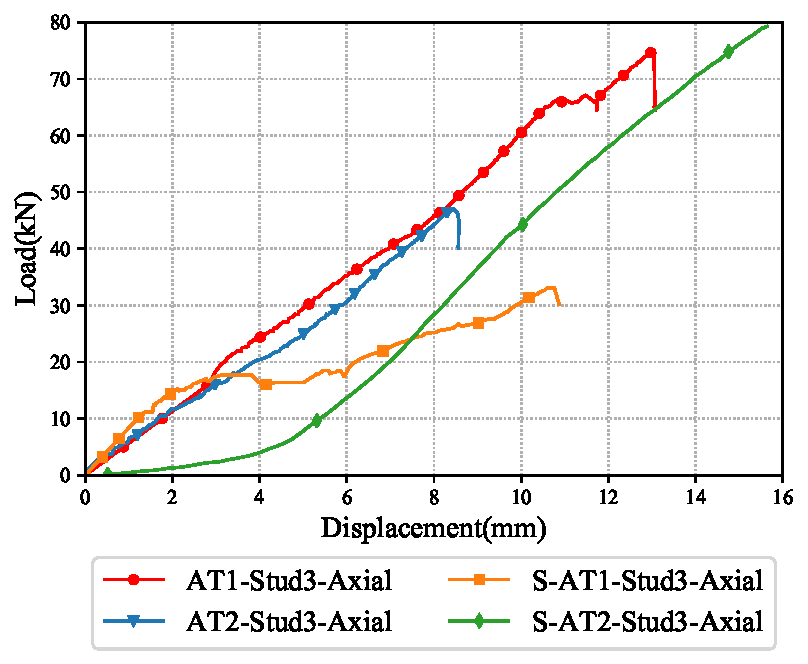
\includegraphics[scale=0.7]{90mm-Axial-comparison.pdf}\\
		\caption{Comparison of applied load versus axial displacement curves - 90 mm studs}
		\label{fig:90mm-comparison-ambient}
\end{figure}
\begin{figure}[!htbp]
	\centering
			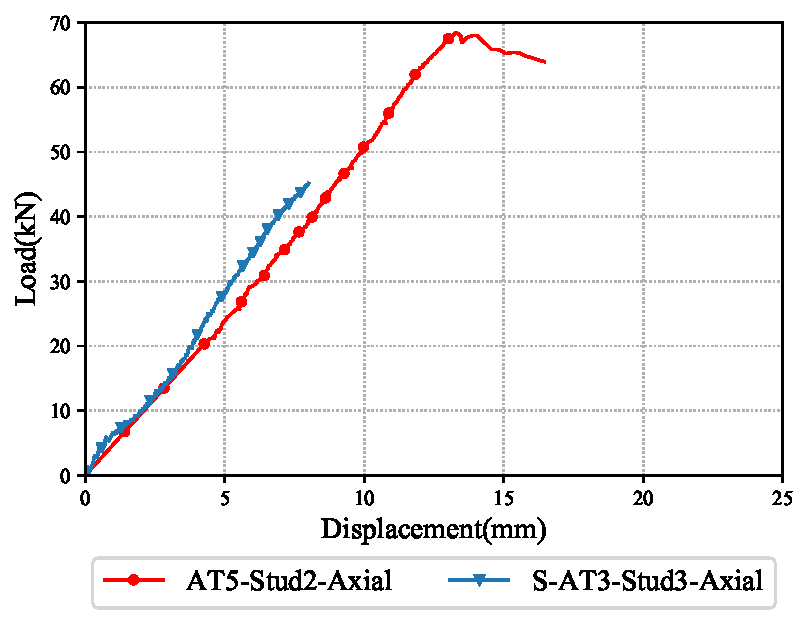
\includegraphics[scale=0.7]{150mm-Axial-comparison.pdf}\\
		\caption{Comparison of applied load versus axial displacement curves - 150 mm studs}
		\label{fig:150mm-comparison-ambient}
\end{figure}
\begin{figure}[!htbp]
	\centering
			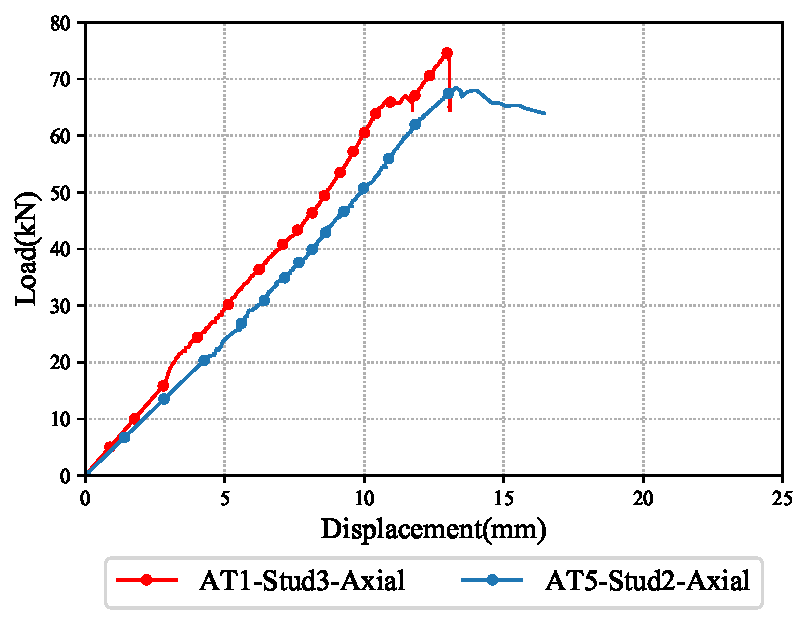
\includegraphics[scale=0.7]{AT1-AT5-comparison.pdf}\\
		\caption{Comparison of applied load versus axial displacement curves from Test-AT1 and AT5}
		\label{fig:AT1-AT5-comparison-ambient}
\end{figure}

The ultimate axial compression capacity of 79.24 kN was recorded in single stud wall with stud thickness of 1.15 mm (S-AT2). The least axial compression capacity of 33.1 kN was recorded for the single stud wall with 0.75 mm stud (S-AT1). In single stud LSF walls, the plasterboards provide effective lateral restraints preventing the in plane (minor axis) buckling of studs. As the webs of studs locally buckle, the out of plane plasterboard restraint is not generally critical under ambient conditions. However, in the case of single stud wall with 150 mm studs the axial compression capacity was 45.43 kN, which is 33.81 kN less than the corresponding single stud wall with 90 mm studs. This is attributed to the wider web depth in 150 mm studs, resulting in lower axial compression capacity.

In the case of double stud LSF walls the effective plasterboard restraints are provided to one flange only on each stud row. The inner stud flanges in the LSF wall are restrained at 1 m intervals through noggings. This results in inadequate in-plane plasterboard restraints to the studs resulting in reduced axial compression capacity. If the single stud wall Test-S-AT1 is compared with the double stud wall Test-AT2, the stud thicknesses were 0.75 mm in both cases, the axial compression capacity was 23.54 kN per stud (47.08/2) in double stud wall Test-AT2, whereas it was 33.10 kN in single stud wall Test-S-AT1. The reduction in axial compression capacity was 9.56 kN. This emphasises the importance of effective plasterboard restraint to both stud flanges in LSF walls under axial compression loading.

Another finding was the double stud wall Test-AT4 with 70 mm studs resulted in a higher axial compression capacity of 86.21 kN (86.21/2 = 43.10 kN per stud) in comparison with double stud wall with 90 mm studs (Test-AT1) resulting in an axial compression capacity of 73.0 kN (73.0/2 = 36.50 kN per stud). Despite having the same stud thickness and wall configuration, the 70 mm double stud wall resulted in higher axial compression capacity. This can be attributed to higher slenderness of 90 mm studs in comparison with the 70 mm studs. However, the axial compression capacity of 90 mm single stud LSF wall lined with plasterboard on both sides resulted in a higher compression capacity in comparison with double and staggered stud walls 

Comparing the LSF walls with 150 mm cavity depth, the axial compression capacity was 68.49 kN in staggered stud wall Test-AT5 and 45.43 kN in 150 mm single stud wall Test-S-AT3. This is a significant reduction in the axial compression capacity. It is to note that the stud spacing was staggered with an effective spacing of 300 mm in staggered stud wall Test-AT5 while the stud spacing was 600 mm in 150 mm wide single stud wall Test-S-AT3. Also, the omega noggings were connected through the stud webs in Test-AT5 while no nogging restraints were provided for Test-S-AT3. Despite having a higher stud thickness of 1.15 mm the 150 mm wall Test-S-AT3 resulted in a reduced axial compression capacity. 

\Cref{fig:AT1-AT5-comparison-ambient} shows the applied load versus displacement curves comparison from test AT1 and AT5. The axial compression capacity from Test-AT1 was 73 kN (73.0/2 = 36.50 kN per stud) while the Test-AT5 gave 68.49 kN (68.49/2 = 34.25 kN per stud). Despite the difference in wall configuration and restraint conditions the staggered stud wall performed equal to that of double stud wall. This is attributed to the omega noggings supporting the stud webs, thereby providing equal restraints in comparison with conventional noggings connecting the stud flanges. Through the staggered stud arrangement the overall wall thickness was maintained at 214 mm (150 mm cavity depth + (32 $\times$ 4 $=$ 64 mm plasterboard thickness)) while it was 264 mm (200 mm cavity depth + (32 $\times$ 4 $=$ 64 mm plasterboard thickness)) in the case of a similar double stud LSF wall configuration. This can result in significant savings in the effective floor space in the construction industry and also achieving similar axial compression capacity. 

\section{Tensile Coupon Tests}\label{sec:tensile-coupon}

Tensile coupon tests were conducted to determine the Young's Modulus and yield strength of the steel studs. Details of the tensile coupons are given in \Cref{fig:tensile-coupon-details}. Tensile coupons were cut from the web and flanges of the studs at three locations along the 3 m long studs. Tensile coupon tests were conducted using Instron testing machine which operates on Bluehill software. Extensometers were used to measure the strain. \Cref{fig:tensile-coupon-details} shows the details of tensile coupons.  
\begin{figure}[!htbp]
	\centering
			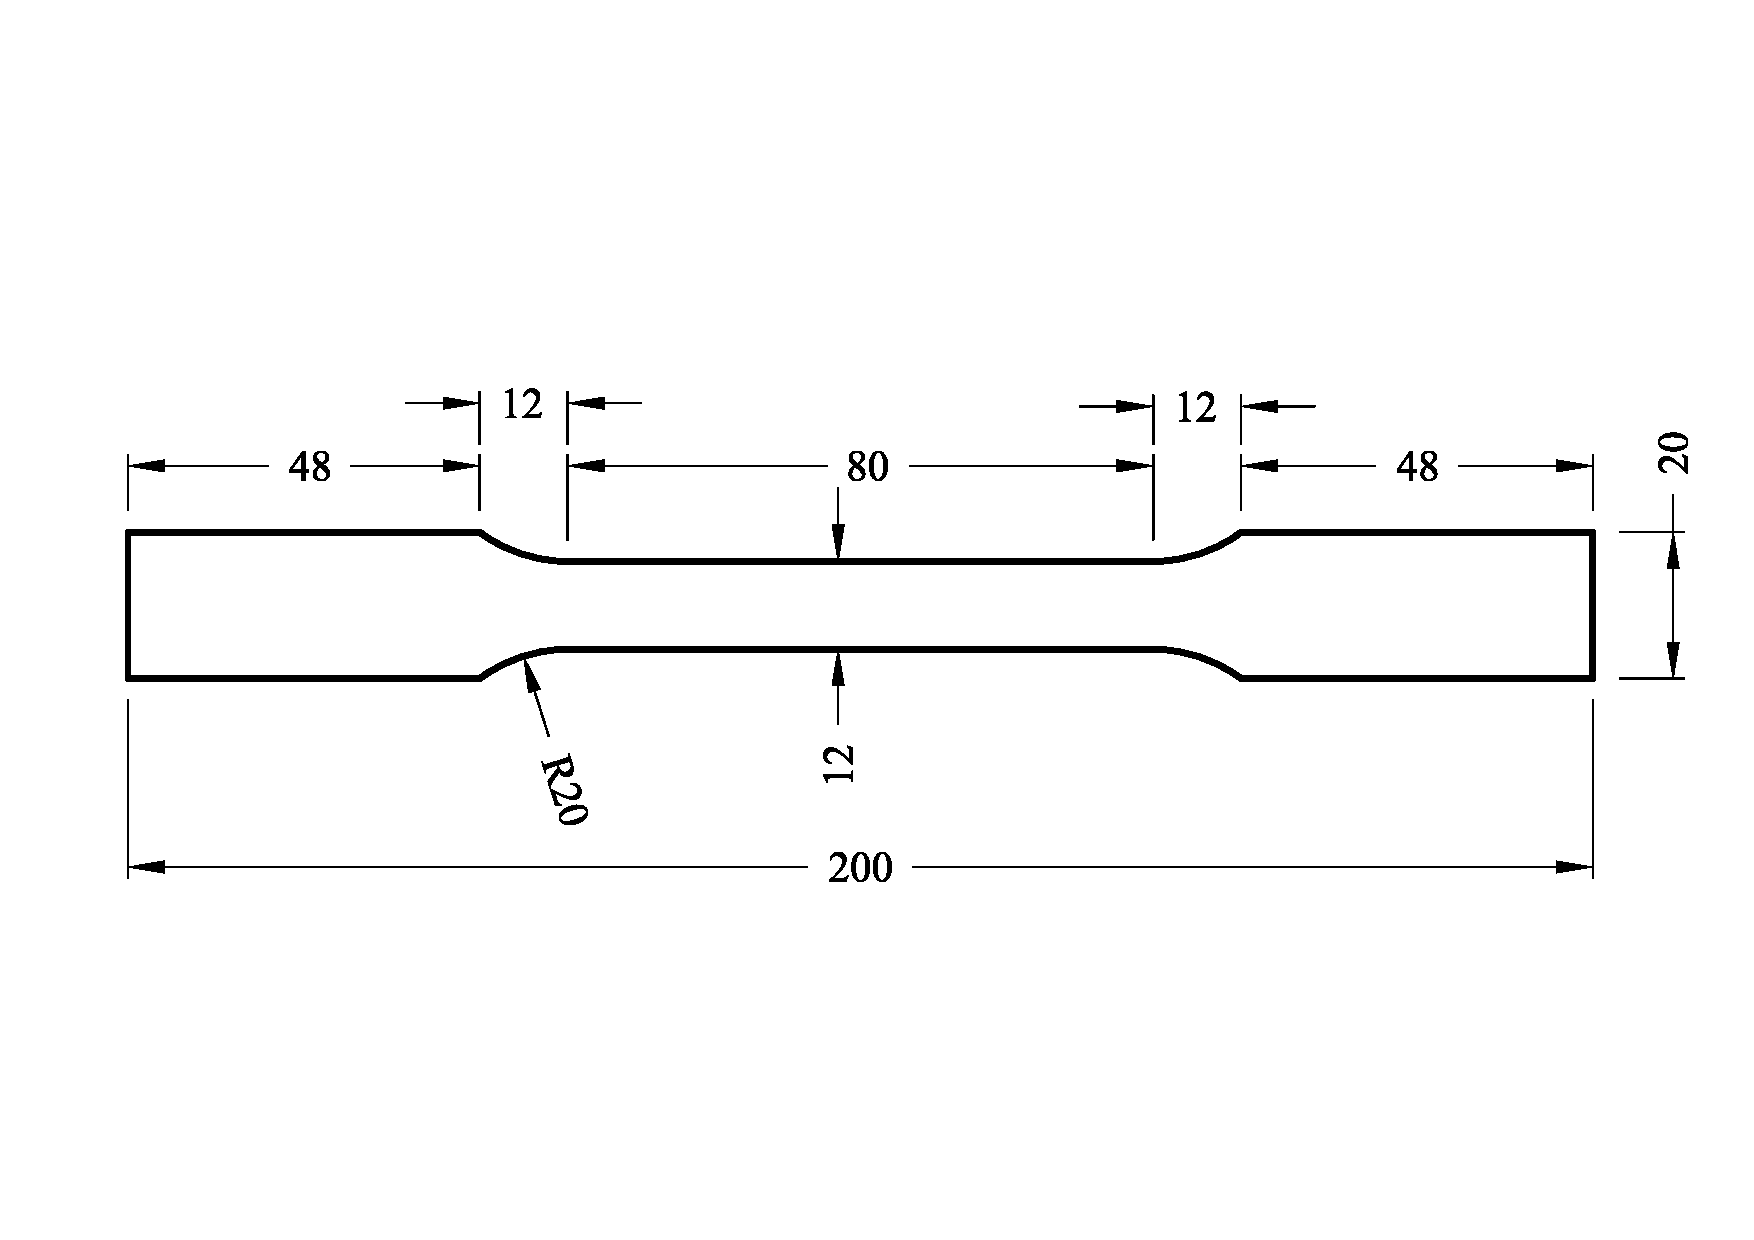
\includegraphics[scale=0.4]{tensile-coupon-details}\\
		\caption{Tensile coupon details}
		\label{fig:tensile-coupon-details}
\end{figure}
\begin{figure}[!htbp]
	\centering
			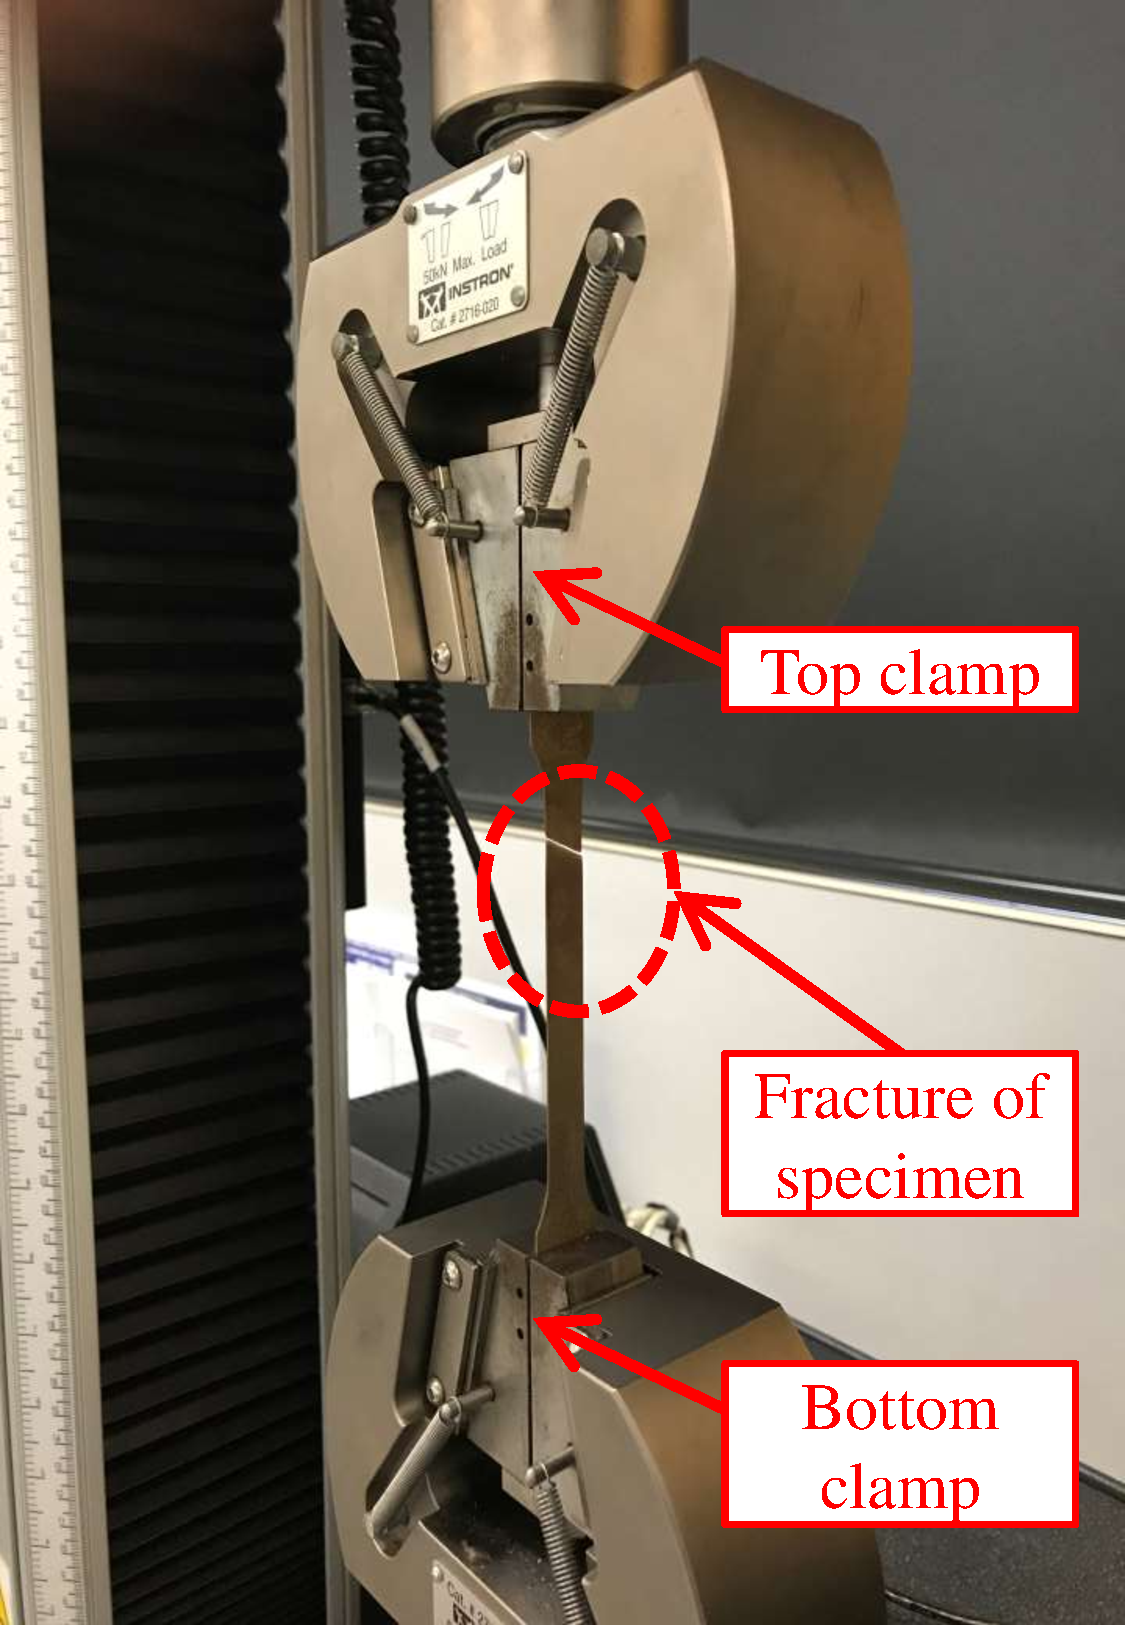
\includegraphics[scale=0.3]{Coupon-test-setup.pdf}\\
		\caption{Tensile coupon test set-up}
		\label{fig:tensile-coupon-test-setup}
\end{figure}
% Table generated by Excel2LaTeX from sheet '0.75'
\begin{table}
	\centering
	\caption{Tensile coupon test results of 0.75 mm thick studs}
	  \begin{tabular}{cccc}
	  \toprule
	  \multicolumn{1}{p{2.145em}}{\centering Test\newline{}No} & 
	  \multicolumn{1}{p{4.07em}}{\centering Coupon Sample\newline{}Location} & 
	  \multicolumn{1}{p{7.07em}}{\centering Young's\newline{}Modulus (GPa)} & 
	  \multicolumn{1}{p{7.145em}}{\centering Yield\newline{}Strength (MPa)} \\
	  \midrule
	  1    & Web  &  202.5 & 634.4 \\
	  2    & Web  &  232.3 & 658.4 \\
	  3    & Web  &  220.5 & 633.0 \\
	  4    & Web  &  214.3 & 642.9 \\
	  5    & Web  &  218.2 & 643.6 \\
	  6    & Web  &  212.9 & 642.9 \\
	  7    & Flange &  212.4 & 648.7 \\
	  8    & Flange &  216.4 & 658.3 \\
	  9    & Flange &  217.5 & 660.5 \\
	  \midrule
	  \multicolumn{2}{c}{Average} & 216.3 & 646.9 \\
	  \bottomrule
	  \end{tabular}%
	\label{tab:075-coupon-results}%
  \end{table}%
  % Table generated by Excel2LaTeX from sheet '0.95'
\begin{table}
\centering
\caption{Tensile coupon test results of 0.95 mm thick studs}
	\begin{tabular}{ccccc}
	\toprule
	\multicolumn{1}{p{2.145em}}{\centering Test\newline{}No} & 
	\multicolumn{1}{p{4.07em}}{\centering Coupon Sample\newline{}Location} & 
	\multicolumn{1}{p{7.07em}}{\centering Young's\newline{}Modulus (GPa)} & 
	\multicolumn{1}{p{7.145em}}{\centering Yield\newline{}Strength (MPa)} \\
	\midrule
	10   & Web  &  216.5 & 612.9 \\
	11   & Web  &  219.1 & 623.7 \\
	12   & Web  &  202.8 & 622.9 \\
	13   & Flange &  217.9 & 620.7 \\
	14   & Flange &  218.6 & 620.6 \\
	15   & Flange &  218.3 & 604.4 \\
	\midrule
	\multicolumn{2}{c}{Average} & 215.5 & 617.5 \\
	\bottomrule
	\end{tabular}%
\label{tab:095-coupon-results}%
\end{table}%
\begin{figure}
\centering
\begin{subfigure}[b]{0.6\textwidth}
	\centering
	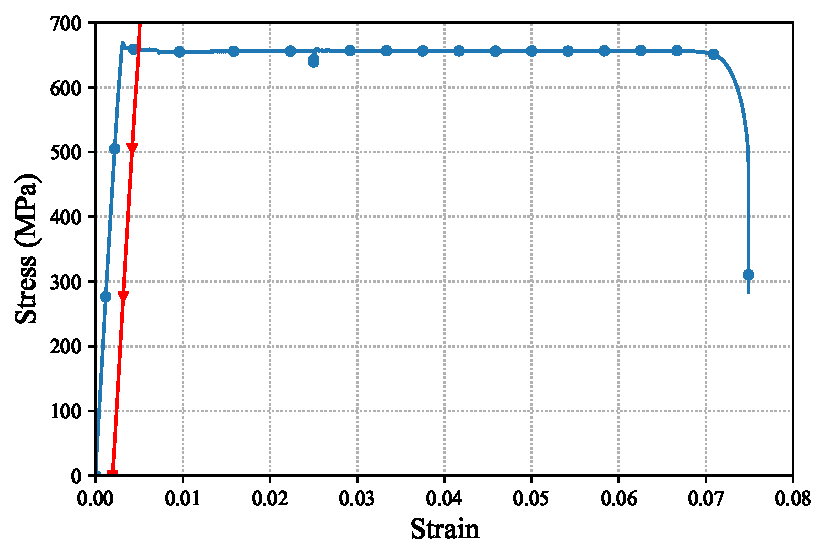
\includegraphics[width=\textwidth]{Test2-Specimen_RawData_5.pdf}
	\caption{}
	\label{subfig:Test2-Specimen_RawData_5}
\end{subfigure}
\begin{subfigure}[b]{0.6\textwidth}
	\centering
	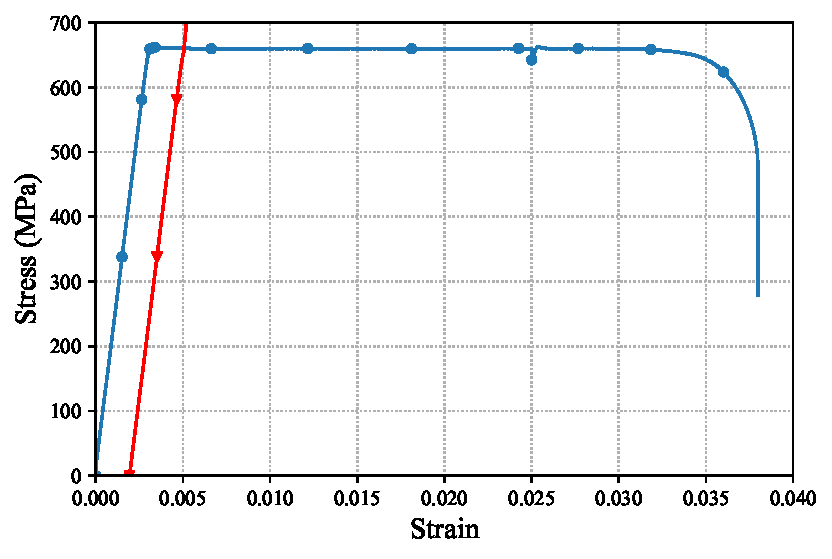
\includegraphics[width=\textwidth]{Test9-Specimen_RawData_4.pdf}
	\caption{}
	\label{subfig:Test9-Specimen_RawData_4}
\end{subfigure}
	\caption{Stress-strain curves from tensile coupon tests of 0.75 mm G550 steel (a) Stud Web (b) Stud Flange}
	\label{fig:075-stress-strain}
\end{figure}
\begin{figure}
	\centering
	\begin{subfigure}[b]{0.6\textwidth}
		\centering
		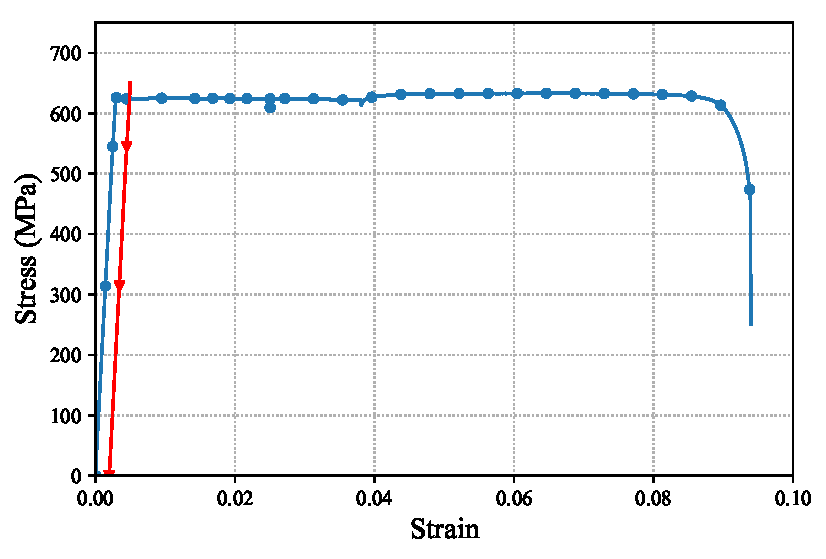
\includegraphics[width=\textwidth]{Test11-Specimen_RawData_6.pdf}
		\caption{}
		\label{subfig:Test11-Specimen_RawData_6}
	\end{subfigure}
		\label{fig:095-stress-strain-a}
\end{figure}
\begin{figure}
	\ContinuedFloat
	\centering
	\begin{subfigure}[b]{0.6\textwidth}
		\centering
		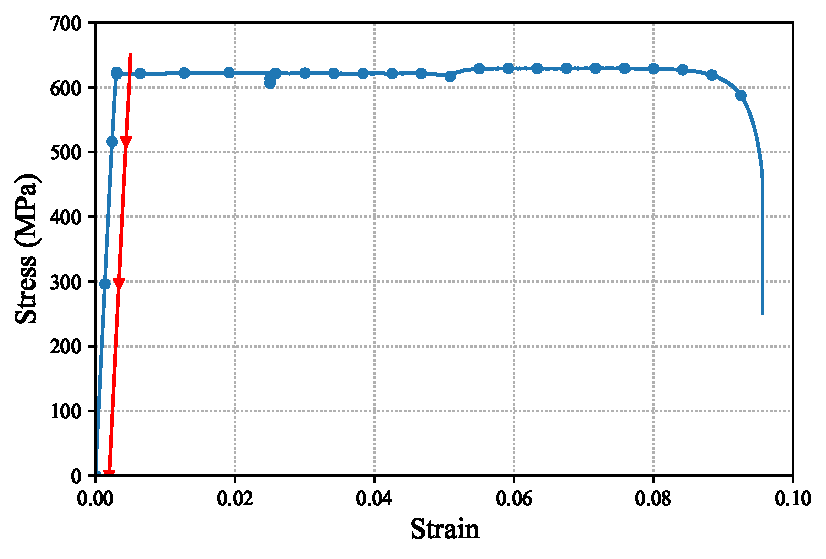
\includegraphics[width=\textwidth]{Test13-Specimen_RawData_8.pdf}
		\caption{}
		\label{subfig:Test13-Specimen_RawData_8}
	\end{subfigure}
		\caption{Stress-strain curves from tensile coupon tests of 0.95 mm G550 steel (a) Stud Web (b) Stud Flange}
		\label{fig:095-stress-strain}
\end{figure}

\Cref{fig:tensile-coupon-test-setup} shows the tensile coupon test set-up. Details of the tensile coupon tests are shown in \Cref{tab:075-coupon-results,tab:095-coupon-results}. Fifteen tensile coupon tests were conducted to determine the Young's Modulus and yield strength of the steel used in the ambient temperature capacity wall tests. \Cref{fig:075-stress-strain,fig:095-stress-strain} show the stress-strain curves obtained for 0.75 mm and 0.95 mm studs while \Cref{tab:075-coupon-results,tab:095-coupon-results} give the measured Young's modulus and yield strength values. The average Young's Modulus and yield strength of 0.75 mm thick studs were 216.4 GPa and 647.0 MPa respectively. Likewise, for 0.95 mm thick steel, the average Young's Modulus and yield strength were 215.6 GPa and 617.5 MPa, respectively. The yield strength of 0.75 mm thick steel was higher in comparison with 0.95 mm steel. 

\section[Design Capacity Predictions Based on Direct Strength Method (DSM)]{Design Capacity Predictions Based on \\Direct Strength Method (DSM)}

Conducting full-scale tests to determine the ambient capacity of the LSF wall configurations are precise but are expensive and time consuming. Therefore researchers have developed equations based on experimental and numerical studies to determine the ambient temperature axial compression capacities of these thin-walled LSF walls. Cold-formed steel members are generally designed based on the Effective Width Method (EWM) or the Direct Strength Method (DSM). The DSM is widely used in recent times over EWM due to less cumbersome calculations involved as stated by \citet{Yu2007,Schafer2008b,Shahbazian2011,Shahbazian2012}. Suitable DSM equations were successfully developed and used by \citet{Kesawan2016} to predict the reduced load bearing capacities of Hollow Flange Channel Section (HFC) studs when exposed to non-uniform temperature distributions during standard fire tests. Their applicability to other cold-formed steel sections such as Lipped Channel and Web Stiffened channel sections were then verified by \citet{Rusthi2018}. The DSM equations have been recently included in AS/NZS 4600 \citet{ASNZ4600}. These two research studies \citet{Kesawan2016,Rusthi2018} have enabled the use of DSM based design equations to determine the load bearing capacity of cold-formed steel studs at ambient temperatures. This research has also investigated the applicability of these design equations to predict the ambient temperature capacities of the double and staggered stud LSF wall configuration considered for experimental investigation in this chapter.

To determine the ambient temperature capacities through DSM equations, parameters such as stud dimensions, mechanical properties and load factors from elastic buckling analysis are required. The stud dimensions were determined through the data specification sheet from the manufacturer and the mechanical properties were determined through tensile coupon tests discussed previously in \Cref{sec:tensile-coupon}. The load factors were determined through elastic buckling analysis conducted using Constrained and Unconstrained Finite Strip Method (CUFSM) software developed by \citet{Li2010a}. The stud sections are modelled using centre line dimensions and appropriate boundary conditions are assigned to the stud flanges and the finite strip analysis was performed using CUFSM. It is to be noted that CUFSM possesses capabilities to perform elastic buckling analysis corresponding to cross-section only. Therefore, the lateral restraints provided at the flanges to simulate intermittent plasterboard and nogging restraints are considered throughout the full length of the stud instead of the intermittent locations. This shortcoming might result in conservative results when the load factors are substituted in the AS 4600, (\cite{ASNZ4600}) based design capacity equations. \Cref{fig:signature-curve} shows the signature curve outputs The output from the CUFSM in the form of signature curves highlighting the important load factors corresponding to different buckling modes are shown in \Cref{fig:signature-curve}.     
\begin{figure}
	\centering
	\begin{subfigure}[b]{0.6\textwidth}
		\centering
		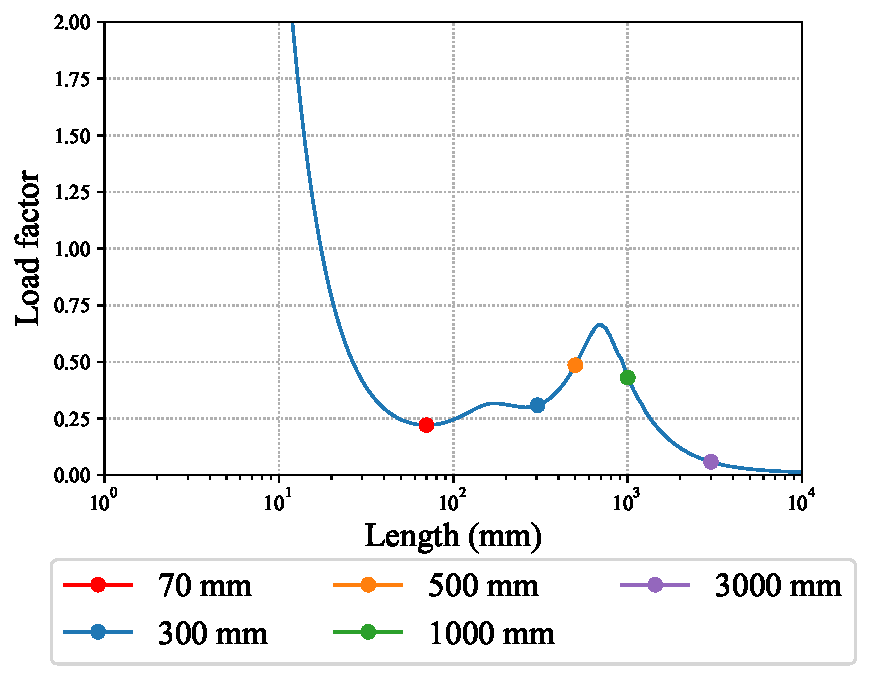
\includegraphics[width=\textwidth]{90-095-signature.pdf}
		\caption{}
		\label{subfig:90-095-signature}
	\end{subfigure}
	\begin{subfigure}[b]{0.6\textwidth}
		\centering
		\includegraphics[width=\textwidth]{90-075-signature.pdf}
		\caption{}
		\label{subfig:90-075-signature}
	\end{subfigure}
	\begin{subfigure}[b]{0.6\textwidth}
		\centering
		\includegraphics[width=\textwidth]{70-095-signature.pdf}
		\caption{}
		\label{subfig:70-095-signature}
	\end{subfigure}
		% \caption{Signature curves from finite strip analysis (CUFSM) for Test (a) AT1 (b) AT2 (c) AT4 (d) AT5}
		\label{fig:signature-curve-a}
\end{figure}
\begin{figure}
	\ContinuedFloat
	\centering
	\begin{subfigure}[b]{0.6\textwidth}
		\centering
		\includegraphics[width=\textwidth]{90-095-st-signature.pdf}
		\caption{}
		\label{subfig:90-095-st-signature}
	\end{subfigure}
		\caption{Signature curves from finite strip analysis (CUFSM) for Tests (a) AT1 (b) AT2 (c) AT4 (d) AT5}
		\label{fig:signature-curve}
\end{figure}
\begin{figure}
	\centering
	\begin{subfigure}[b]{0.15\textwidth}
		\centering
		\includegraphics[width=\textwidth]{90-095-70mm.pdf}
		\caption{}
		\label{subfig:90-095-70mm}
	\end{subfigure}
	\begin{subfigure}[b]{0.15\textwidth}
		\centering
		\includegraphics[width=\textwidth]{90-095-300mm.pdf}
		\caption{}
		\label{subfig:90-095-300mm}
	\end{subfigure}
	\begin{subfigure}[b]{0.15\textwidth}
		\centering
		\includegraphics[width=\textwidth]{90-095-500mm.pdf}
		\caption{}
		\label{subfig:90-095-500mm}
	\end{subfigure}
	\begin{subfigure}[b]{0.18\textwidth}
		\centering
		\includegraphics[width=\textwidth]{90-095-1000mm.pdf}
		\caption{}
		\label{subfig:90-095-1000mm}
	\end{subfigure}
	\begin{subfigure}[b]{0.18\textwidth}
		\centering
		\includegraphics[width=\textwidth]{90-095-3000mm.pdf}
		\caption{}
		\label{subfig:90-095-3000mm}
	\end{subfigure}
		\caption{Buckling modes from finite strip analysis (CUFSM) for Test-AT1 at different lengths (a) 70 mm (b) 300 mm (c) 500 mm (d) 1000 mm (e) 3000 mm}
		\label{fig:90-095-CUFSM-buckling}
\end{figure}
\begin{figure}
	\centering
	\begin{subfigure}[b]{0.15\textwidth}
		\centering
		\includegraphics[width=\textwidth]{90-075-70mm.pdf}
		\caption{}
		\label{subfig:90-075-70mm}
	\end{subfigure}
	\begin{subfigure}[b]{0.18\textwidth}
		\centering
		\includegraphics[width=\textwidth]{90-075-300mm.pdf}
		\caption{}
		\label{subfig:90-075-300mm}
	\end{subfigure}
	\begin{subfigure}[b]{0.18\textwidth}
		\centering
		\includegraphics[width=\textwidth]{90-075-1000mm.pdf}
		\caption{}
		\label{subfig:90-075-1000mm}
	\end{subfigure}
	\begin{subfigure}[b]{0.18\textwidth}
		\centering
		\includegraphics[width=\textwidth]{90-075-3000mm.pdf}
		\caption{}
		\label{subfig:90-075-3000mm}
	\end{subfigure}
		\caption{Buckling modes from finite strip analysis (CUFSM) for Test-AT2 at different lengths (a) 70 mm (b) 300 mm (c) 1000 mm (d) 3000 mm}
		\label{fig:90-075-CUFSM-buckling}
\end{figure}
\begin{figure}
	\centering
	\begin{subfigure}[b]{0.15\textwidth}
		\centering
		\includegraphics[width=\textwidth]{70-095-50mm.pdf}
		\caption{}
		\label{subfig:70-095-50mm}
	\end{subfigure}
	\begin{subfigure}[b]{0.15\textwidth}
		\centering
		\includegraphics[width=\textwidth]{70-095-300mm.pdf}
		\caption{}
		\label{subfig:70-095-300mm}
	\end{subfigure}
	\begin{subfigure}[b]{0.18\textwidth}
		\centering
		\includegraphics[width=\textwidth]{70-095-1000mm.pdf}
		\caption{}
		\label{subfig:70-095-1000mm}
	\end{subfigure}
	\begin{subfigure}[b]{0.18\textwidth}
		\centering
		\includegraphics[width=\textwidth]{70-095-3000mm.pdf}
		\caption{}
		\label{subfig:70-095-3000mm}
	\end{subfigure}
		\caption{Buckling modes from finite strip analysis (CUFSM) for Test-AT4 at different lengths (a) 50 mm (b) 300 mm (c) 1000 mm (d) 3000 mm}
		\label{fig:70-095-CUFSM-buckling}
\end{figure}
\begin{figure}
	\centering
	\begin{subfigure}[b]{0.15\textwidth}
		\centering
		\includegraphics[width=\textwidth]{90-095-st-40mm.pdf}
		\caption{}
		\label{subfig:90-095-st-40mm}
	\end{subfigure}
	\begin{subfigure}[b]{0.15\textwidth}
		\centering
		\includegraphics[width=\textwidth]{90-095-st-200mm.pdf}
		\caption{}
		\label{subfig:90-095-st-200mm}
	\end{subfigure}
	\begin{subfigure}[b]{0.15\textwidth}
		\centering
		\includegraphics[width=\textwidth]{90-095-st-300mm.pdf}
		\caption{}
		\label{subfig:90-095-st-300mm}
	\end{subfigure}
	\begin{subfigure}[b]{0.15\textwidth}
		\centering
		\includegraphics[width=\textwidth]{90-095-st-1000mm.pdf}
		\caption{}
		\label{subfig:90-095-st-1000mm}
	\end{subfigure}
	\begin{subfigure}[b]{0.15\textwidth}
		\centering
		\includegraphics[width=\textwidth]{90-095-st-3000mm.pdf}
		\caption{}
		\label{subfig:90-095-st-3000mm}
	\end{subfigure}
		\caption{Buckling modes from finite strip analysis (CUFSM) for Test-AT5 at different lengths (a) 40 mm (b) 200 mm (c) 300 mm (d) 1000 mm (e) 3000 mm}
		\label{fig:90-095-st-CUFSM-buckling}
\end{figure}

% Table generated by Excel2LaTeX from sheet 'Table-measured'
\begin{table}[htbp]
	\centering
	\caption{Ultimate axial compression capacities from DSM predictions and experiment}
	  \begin{tabular}{ccccc}
	  \toprule
	  \multirow{2}[4]{*}{Test} & \multicolumn{3}{c}{Ultimate Axial Compression Capacities (kN)} & \multirow{2}[4]{*}{Difference} \\
  \cmidrule{2-4}          & DSM (per stud) & DSM combined & Experiment &  \\
	  \midrule
	  AT1   & 25.9  & 51.8  & 73    & 21.2 \\
	  AT2   & 17.64 & 35.28 & 47.08 & 11.8 \\
	  AT4   & 17.8  & 35.6  & 86.21 & 50.61 \\
	  AT5   & 37.86 & 75.72 & 68.49 & -7.23 \\
	  \bottomrule
	  \end{tabular}%
	\label{tab:dsm-ambient}%
  \end{table}%
  
CUFSM analysis was conducted on three stud dimensions 90 $\times$ 0.95 mm, 90 $\times$ 0.75 mm, 70 $\times$ 0.95 mm corresponding to ambient temperature capacity Tests-AT1, AT2, AT4 and AT5. Test-AT3 was not considered for the CUFSM analysis as the stud dimensions were similar to that of Test-AT2. Also, for Test-AT5 90 $\times$ 0.95 mm stud was used wherein the restraints were provided on the web in addition to the one flange provided in other models as shown in \Cref{fig:90-095-CUFSM-buckling,fig:90-075-CUFSM-buckling,fig:70-095-CUFSM-buckling,fig:90-095-st-CUFSM-buckling} which includes the buckling modes of the studs from CUFSM analysis. For the DSM based design calculations, the lowest load factor from the signature curves are extracted to determine the ambient temperature compression capacities of the conducted full-scale tests. Local buckling was the lowest failure mode in all the studs as inferred from the signature curves shown in \Cref{fig:signature-curve}. The local buckling factor from the signature curve corresponding to Tests-AT1 and AT2 occurred at half wave lengths of 70 mm while it was 50 mm and 40 mm for Tests-T4 and T5. The corresponding load factors were incorporated in the DSM equations and the ultimate compression capacities of the stud sections were determined and is shown in \Cref{tab:dsm-ambient}. 

Single studs were modelled in CUFSM to determine the load factor for substitution in the DSM equations. Therefore, the arrived capacities are doubled to determine the ultimate axial compression capacity of a stud set. The axial compression capacity predictions from the AS 4600 based DSM equation resulted in lower capacities in comparison with the experiments except Test-AT5. The DSM predictions resulted a maximum ambient temperature axial compression capacity for Test-AT5 (staggered stud wall with 90 $\times$ 0.95 mm studs). However, the experiment gave a maximum axial compression capacity for Test-AT1. This was attributed to the continuous restraints considered on the stud web and flanges resulting in higher local bucking load factors in comparison with the double stud wall Test-AT1. Since the continuous restrain is considered only on one flange, in Test-AT1, the local buckling load factor was lower and resulted in a reduced ultimate axial compression capacity. Likewise the DSM based ultimate compression capacity for Test-AT5 was lower than the experiment. The difference in predicted capacity and experiment for Test-AT4 may be attributed by various reasons which includes the load sharing to the stiffened nested edge studs and may also be due to the higher yield strength of steel studs used in the test wall. This was possible as the studs for Test-AT4 were procured from a different batch of studs. This shows the need to develop a finite element (FE) structural model to better predict the axial compression capacities of the double and staggered stud LSF wall systems and will be discussed in \Cref{ch:FE-Structural}. There also prevails a limitation in assigning intermittent lateral restraints to the stud flanges and near the service holes in the web in determining the load factors through CUFSM.

\section{Summary of Findings}

The following findings can be drawn from the ambient temperature capacity tests on double and staggered stud LSF walls and tensile coupon tests.
\begin{itemize}
	\item Axial compression capacity of LSF wall is dependent on the thickness and depth of the studs.
	\item The effect of plasterboards on the stud flanges providing in-plane lateral restraints significantly influences the axial compression capacity of single stud LSF walls. The absence of effective plasterboard restraints on the inner stud flanges in double stud walls greatly affects the axial compression capacity of double stud LSF walls.
	\item In the case of staggered stud LSF walls, despite the absence of plasterboard restraint on one flange, the omega noggings connecting the stud webs provide significant in-plane lateral restraints to the studs and together with additional end cleats at the supports gave resulting in a similar axial compression capacity in comparison with double stud LSF walls.
	\item The axial compression capacity of plasterboard lined double stud walls is significantly higher for walls with 70 mm studs in comparison with 90 mm studs with the same thickness. This is attributed to the increased plate slenderness of 90 mm studs. 
	\item Tensile tests of coupons taken from G550 steel studs show that the minimum guaranteed yield strength of 550 MPa is achieved in all the tests. 0.75 mm steel has a higher yield strength in comparison with 0.95 mm steel despite the same grade of steel. This is because of the higher cold work in steel with lower thicknesses. However, the Young's Modulus is almost similar irrespective of the thickness. The Young's Modulus and yield strength results from the coupon tests reported in this chapter can be used in the numerical analysis of LSF walls. 
	\item Ultimate compression capacities predicted from the new DSM equations in AS 4600 resulted in reasonable agreement for double stud wall Tests-AT1, AT2 and staggered stud wall Test-AT5. However, the design capacity predictions for AT4 was lower in comparison with the experiment. This may be attributed to the load sharing in the studs due to nesting of the edge studs and may also be due to the difference in mechanical properties of the steel used for Test-AT4. The limitation of providing intermittent lateral restraints to determine the load factors for DSM calculation needs to be addressed to better determine the axial compression capacities of the studs. 
\end{itemize}
  
  
  
